\documentclass[11pt,a4paper,copyright]{google}

\usepackage{upquote}
\usepackage{tikz}
\usetikzlibrary{arrows.meta,positioning,calc,shapes.geometric}
\usepackage[skins,breakable]{tcolorbox}
\usepackage[capitalize,noabbrev]{cleveref}

% Tonal Architectural Palette (Non-Evaluative Structural Colors)
\definecolor{gBlue}{HTML}{1A73E8}
\definecolor{gBlueBg}{HTML}{E8F0FE}
\definecolor{gNavy}{HTML}{174EA6}
\definecolor{gNavyBg}{HTML}{EDF2FA}
\definecolor{gSlate}{HTML}{334155}
\definecolor{gSlateBg}{HTML}{F1F5F9}
\definecolor{gGray}{HTML}{64748B}
\definecolor{gGrayBg}{HTML}{F8FAFC}
% Evaluative Status Colors (Strictly for Pass/Fail Thresholds)
\definecolor{evalPass}{HTML}{137333}
\definecolor{evalPassBg}{HTML}{E6F4EA}
\definecolor{evalFail}{HTML}{C5221F}
\definecolor{evalFailBg}{HTML}{FCE8E6}

\newtcolorbox{conceptbox}[1]{%
  enhanced, breakable,
  colback=gBlueBg!55!white, colframe=gBlueBg!55!white,
  boxrule=0pt, arc=3pt, boxsep=0pt,
  borderline west={2.5pt}{0pt}{gBlue},
  left=12pt, right=12pt, top=14pt, bottom=9pt,
  title={#1},
  fonttitle=\sffamily\bfseries\footnotesize,
  coltitle=white,
  attach boxed title to top left={xshift=9pt,yshift=-6pt},
  boxed title style={
    colback=gNavy, colframe=gNavy,
    boxrule=0pt, arc=0pt, outer arc=0pt, boxsep=0pt,
    left=6pt, right=6pt, top=2.4pt, bottom=2.4pt}}

\hypersetup{
    colorlinks=true,
    linkcolor=gNavy,
    citecolor=gBlue,
    urlcolor=gBlue,
    pdftitle={Unifying Inner-Loop Execution Harnesses and Outer-Loop Specification State for Autonomous Software Engineering},
    pdfauthor={Alejandro Kaspar, Hader Ceron, Joaquin Menendez, Nacho Villaluenga - Google Cloud Consulting}
}

\newcolumntype{L}[1]{>{\raggedright\arraybackslash}p{#1}}
\newcolumntype{C}[1]{>{\centering\arraybackslash}p{#1}}
\newcolumntype{R}[1]{>{\raggedleft\arraybackslash}p{#1}}
\newcolumntype{Y}{>{\raggedright\arraybackslash}X}

\setlength{\parskip}{0.48em plus 0.22em minus 0.08em}
\setlength{\parindent}{0pt}
\setlength{\textfloatsep}{10pt plus 4pt minus 3pt}
\setlength{\floatsep}{8pt plus 3pt minus 2pt}
\setlength{\intextsep}{8pt plus 3pt minus 2pt}
\flushbottom
\emergencystretch=3em

\newtheorem{definition}{Definition}
\newtheorem{proposition}{Proposition}

\title{Unifying Inner-Loop Execution Harnesses and Outer-Loop Specification State for Autonomous Software Engineering}
\author[1]{Alejandro Kaspar}
\author[1]{Hader Ceron}
\author[1]{Joaquin Menendez}
\author[1]{Nacho Villaluenga}
\affil[1]{Google Cloud Consulting, Google}
\correspondingauthor{\{adkaspar, haderceron, joaquinmen, nachov\}@google.com}
\renewcommand{\today}{2026-10-22}






\begin{abstract}
Autonomous coding agents rely on two distinct control loops during software development. The inner execution loop governs how an agent clarifies task ambiguities, probes boundary conditions, authors unit tests, and verifies code edits under tamper-proof test locks. The outer specification loop governs how system requirements, architectural contracts, and historical delta changes persist across multi-milestone repository evolution. Existing frameworks address these loops in isolation: inner-loop harnesses optimize single-turn task verification without maintaining a synchronized specification state across sprints, whereas outer-loop specification frameworks structure requirement documents without enforcing contrastive boundary probing or read-only test locks during execution. We introduce a unified dual-loop architecture that couples a Contract-Locked Dual-Stage Inner Execution Harness with a Two-Plane Delta-Merged Outer Specification State Machine. Across 252 blind multi-subagent benchmark trials instantiated with \texttt{Gemini 3.8 Flash} (312 subagent invocations including fresh-context cold auditors) spanning four untouched upstream inner-loop benchmarks (\texttt{SWE-bench Verified}, \texttt{Commit0}, \texttt{BigCodeBench v0.1.2}, and \texttt{EvalPlus HumanEval+} $80\times$ stress tests; 240 trials) and a five-milestone longitudinal specification evolution benchmark (\texttt{Commit0-Evo} on \texttt{TinyDB}; 12 multi-milestone trials evaluated across 60 sequential milestone checks), our Contract-Locked Dual-Stage Harness reduces baseline test tampering from $18.3 \pm 2.9\%$ (\texttt{Procedural TDD}) and $23.3 \pm 2.9\%$ (\texttt{OO-Harness}) to $0.0 \pm 0.0\%$ ($0/60$), raising tamper-free strict pass rate ($\text{Pass}_{\text{strict}} = \text{Oracle} \land \neg\text{Tamper}$) to $91.7 \pm 2.9\%$ ($55/60$, $+21.7\text{ pp}$ over \texttt{OO-Harness} and $+23.4\text{ pp}$ over \texttt{Procedural TDD}) and patched-function AST mutation kill rate to $70.6 \pm 4.6\%$, while our Two-Plane Delta-Merged SSOT achieves $100.0 \pm 0.0\%$ clean-room rebuild and historical rollback accuracy with $0.0\%$ contradiction density and $0.00\text{ bits}$ of behavioral entropy.
\end{abstract}

\begin{document}
\maketitle


\begin{figure}[h!]
\centering
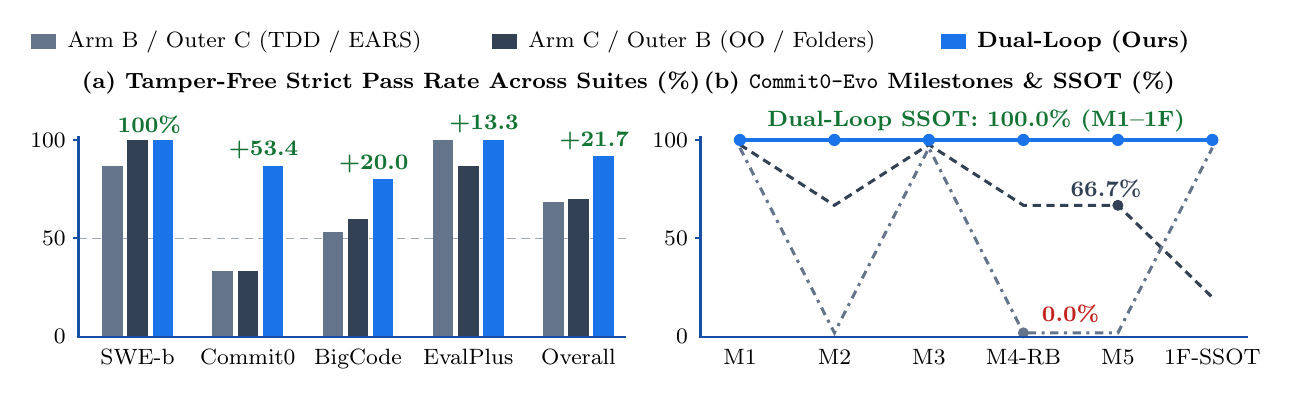
\begin{tikzpicture}[x=1cm,y=1cm,>=Latex]
  % Top Legend Row (y = 4.25, cleanly above all plot elements; all 4 series labeled)
  \fill[gGray] (0.0,4.15) rectangle (0.32,4.35);
  \node[anchor=west, font=\footnotesize, inner sep=1pt] at (0.42,4.25) {Arm B / Outer C (TDD / EARS)};
  \fill[gSlate] (5.85,4.15) rectangle (6.17,4.35);
  \node[anchor=west, font=\footnotesize, inner sep=1pt] at (6.27,4.25) {Arm C / Outer B (OO / Folders)};
  \fill[gBlue] (11.55,4.15) rectangle (11.87,4.35);
  \node[anchor=west, font=\footnotesize, inner sep=1pt] at (11.97,4.25) {\textbf{Dual-Loop (Ours)}};

  % ================= PANEL (a): Tamper-Free Strict Pass Rate Across Upstream Suites =================
  \node[anchor=west, font=\footnotesize, inner sep=1pt] at (0.6,3.72) {\textbf{(a) Tamper-Free Strict Pass Rate Across Suites (\%)}};
  % Y-axis ticks (y = 0.5 is 0%, y = 1.75 is 50%, y = 3.0 is 100%, height = 2.5cm)
  \node[anchor=east, font=\footnotesize, inner sep=1pt] at (0.48,0.5) {0};
  \node[anchor=east, font=\footnotesize, inner sep=1pt] at (0.48,1.75) {50};
  \node[anchor=east, font=\footnotesize, inner sep=1pt] at (0.48,3.0) {100};
  \draw[draw=gNavy, line width=0.8pt] (0.53,1.75) -- (0.60,1.75);
  \draw[draw=gNavy, line width=0.8pt] (0.53,3.00) -- (0.60,3.00);
  \draw[draw=gSlate!45, line width=0.4pt, densely dashed] (0.60,1.75) -- (7.55,1.75);

  % Group 1: SWE-bench (center x = 1.35): Arm B 86.7% (y=2.67), Arm C 100.0% (y=3.00), Arm D 100.0% (y=3.00)
  \fill[gGray] (0.90,0.5) rectangle (1.16,2.67);
  \fill[gSlate] (1.22,0.5) rectangle (1.48,3.00);
  \fill[gBlue] (1.54,0.5) rectangle (1.80,3.00);
  \node[anchor=south, font=\footnotesize, inner sep=1pt, text=evalPass] at (1.50,3.04) {\textbf{100\%}};
  \node[anchor=north, font=\footnotesize, inner sep=1pt] at (1.35,0.38) {SWE-b};

  % Group 2: Commit0 (center x = 2.75): Arm B 33.3% (y=1.33), Arm C 33.3% (y=1.33), Arm D 86.7% (y=2.67)
  \fill[gGray] (2.30,0.5) rectangle (2.56,1.33);
  \fill[gSlate] (2.62,0.5) rectangle (2.88,1.33);
  \fill[gBlue] (2.94,0.5) rectangle (3.20,2.67);
  \node[anchor=south, font=\footnotesize, inner sep=1pt, text=evalPass] at (2.95,2.71) {\textbf{+53.4}};
  \node[anchor=north, font=\footnotesize, inner sep=1pt] at (2.75,0.38) {Commit0};

  % Group 3: BigCodeBench (center x = 4.15): Arm B 53.3% (y=1.83), Arm C 60.0% (y=2.00), Arm D 80.0% (y=2.50)
  \fill[gGray] (3.70,0.5) rectangle (3.96,1.83);
  \fill[gSlate] (4.02,0.5) rectangle (4.28,2.00);
  \fill[gBlue] (4.34,0.5) rectangle (4.60,2.50);
  \node[anchor=south, font=\footnotesize, inner sep=1pt, text=evalPass] at (4.35,2.54) {\textbf{+20.0}};
  \node[anchor=north, font=\footnotesize, inner sep=1pt] at (4.15,0.38) {BigCode};

  % Group 4: EvalPlus 80x (center x = 5.55): Arm B 100.0% (y=3.00), Arm C 86.7% (y=2.67), Arm D 100.0% (y=3.00)
  \fill[gGray] (5.10,0.5) rectangle (5.36,3.00);
  \fill[gSlate] (5.42,0.5) rectangle (5.68,2.67);
  \fill[gBlue] (5.74,0.5) rectangle (6.00,3.00);
  \node[anchor=south, font=\footnotesize, inner sep=1pt, text=evalPass] at (5.75,3.04) {\textbf{+13.3}};
  \node[anchor=north, font=\footnotesize, inner sep=1pt] at (5.55,0.38) {EvalPlus};

  % Group 5: 240-Trial Mean (center x = 6.95): Arm B 68.3% (y=2.21), Arm C 70.0% (y=2.25), Arm D 91.7% (y=2.79)
  \fill[gGray] (6.50,0.5) rectangle (6.76,2.21);
  \fill[gSlate] (6.82,0.5) rectangle (7.08,2.25);
  \fill[gBlue] (7.14,0.5) rectangle (7.40,2.79);
  \node[anchor=south, font=\footnotesize, inner sep=1pt, text=evalPass] at (7.15,2.83) {\textbf{+21.7}};
  \node[anchor=north, font=\footnotesize, inner sep=1pt] at (6.95,0.38) {Overall};

  % Axes for Panel (a) capped at y=3.05 so y=3.00 is visually 100% of the axis
  \draw[draw=gNavy, line width=0.8pt] (0.6,3.05) -- (0.6,0.5) -- (7.55,0.5);

  % ================= PANEL (b): Multi-Milestone Commit0-Evo Trajectory =================
  \node[anchor=west, font=\footnotesize, inner sep=1pt] at (8.5,3.72) {\textbf{(b) \texttt{Commit0-Evo} Milestones \& SSOT (\%)}};
  \node[anchor=east, font=\footnotesize, inner sep=1pt] at (8.38,0.5) {0};
  \node[anchor=east, font=\footnotesize, inner sep=1pt] at (8.38,1.75) {50};
  \node[anchor=east, font=\footnotesize, inner sep=1pt] at (8.38,3.0) {100};
  \draw[draw=gNavy, line width=0.8pt] (8.43,1.75) -- (8.50,1.75);
  \draw[draw=gNavy, line width=0.8pt] (8.43,3.00) -- (8.50,3.00);

  % X coordinates for M1..M5 + 1F: 9.0, 10.2, 11.4, 12.6, 13.8, 15.0
  \node[anchor=north, font=\footnotesize, inner sep=1pt] at (9.0,0.38) {M1};
  \node[anchor=north, font=\footnotesize, inner sep=1pt] at (10.2,0.38) {M2};
  \node[anchor=north, font=\footnotesize, inner sep=1pt] at (11.4,0.38) {M3};
  \node[anchor=north, font=\footnotesize, inner sep=1pt] at (12.6,0.38) {M4-RB};
  \node[anchor=north, font=\footnotesize, inner sep=1pt] at (13.8,0.38) {M5};
  \node[anchor=north, font=\footnotesize, inner sep=1pt] at (15.0,0.38) {1F-SSOT};

  % Trajectory 1: Outer B (Feature Folders, gSlate dashed) -> M1=100% (2.94), M2=66.7% (2.17), M3=100% (2.94), M4-RB=66.7% (2.17), M5=66.7% (2.17), 1F=20% (1.00)
  \draw[draw=gSlate, line width=1.1pt, densely dashed] (9.0,2.94) -- (10.2,2.17) -- (11.4,2.94) -- (12.6,2.17) -- (13.8,2.17) -- (15.0,1.00);
  \fill[gSlate] (13.8,2.17) circle (2.0pt);
  \node[anchor=south, font=\footnotesize, inner sep=1pt, text=gSlate] at (13.65,2.22) {\textbf{66.7\%}};

  % Trajectory 2: Outer C (In-Place EARS, gGray dashdotted) -> M1=100% (2.90), M2=0% (0.55), M3=100% (2.90), M4-RB=0% (0.55), M5=0% (0.55), 1F=100% (2.90)
  \draw[draw=gGray, line width=1.1pt, dashdotted] (9.0,2.90) -- (10.2,0.55) -- (11.4,2.90) -- (12.6,0.55) -- (13.8,0.55) -- (15.0,2.90);
  \fill[gGray] (12.6,0.55) circle (2.0pt);
  \node[anchor=south, font=\footnotesize, inner sep=1pt, text=evalFail] at (13.20,0.64) {\textbf{0.0\%}};

  % Trajectory 3: Outer D (Two-Plane SSOT, Ours, gBlue solid) -> Flat 100.0% across M1..1F-SSOT (y=3.00)
  \draw[draw=gBlue, line width=1.6pt] (9.0,3.00) -- (10.2,3.00) -- (11.4,3.00) -- (12.6,3.00) -- (13.8,3.00) -- (15.0,3.00);
  \foreach \x in {9.0, 10.2, 11.4, 12.6, 13.8, 15.0} {
    \fill[gBlue] (\x,3.00) circle (2.2pt);
  }
  \node[anchor=south, font=\footnotesize, inner sep=1pt, text=evalPass] at (12.0,3.06) {\textbf{Dual-Loop SSOT: 100.0\% (M1--1F)}};

  % Axes for Panel (b) capped at y=3.05
  \draw[draw=gNavy, line width=0.8pt] (8.5,3.05) -- (8.5,0.5) -- (15.45,0.5);
\end{tikzpicture}
\caption{Empirical performance across 252 blind multi-subagent trials on untouched upstream benchmarks. \textbf{(a)} Tamper-free strict pass rate ($\text{Pass}_{\text{strict}} = \text{Oracle} \land \neg\text{Tamper}$) across \texttt{SWE-bench Verified}, \texttt{Commit0}, \texttt{BigCodeBench v0.1.2}, \texttt{EvalPlus HumanEval+} ($80\times$), and the 240-trial aggregate ($3\text{ runs} \times 4\text{ arms} \times 20\text{ tasks}$), comparing Procedural TDD (\texttt{Arm B}, gray), \texttt{OO-Harness} (\texttt{Arm C}, slate), and our Contract-Locked Dual-Stage Harness (\texttt{Arm D}, blue), with percentage-point gains (\textcolor{evalPass}{\textbf{+$\Delta$}}) over \texttt{Arm C} above each bar. \textbf{(b)} Longitudinal \texttt{Commit0-Evo} evaluation across 12 multi-milestone trials on \texttt{TinyDB} showing post-trajectory milestone checks (\texttt{M1}, \texttt{M2}, \texttt{M3}, \texttt{M4-RB} rollback, and \texttt{M5} clean-room rebuild) alongside single-file SSOT consolidation coverage (\texttt{1F-SSOT}): feature-isolated folders (\texttt{Outer B}, dashed slate) drop to $66.7 \pm 57.7\%$ at \texttt{M2}, \texttt{M4-RB}, and \texttt{M5} ($20.0\%$ on \texttt{1F-SSOT}), in-place EARS (\texttt{Outer C}, dash-dotted gray) erases prior cache invariants and drops to $0.0\%$ on \texttt{M2}, \texttt{M4-RB}, and \texttt{M5}, while our Two-Plane SSOT (\texttt{Outer D}, solid blue) maintains $100.0 \pm 0.0\%$ across all checks.}
\label{fig:teaser_chart}
\end{figure}


\section{Introduction}
\label{sec:intro}

For five decades, human-written source code served as the authoritative record of software behavior: compilers and target architectures changed, yet source code defined the exact semantics to reproduce. In AI-driven development, code is generated from natural-language prompts, creating a dual failure mode between prompts that say too little and generated source files that say too much. Prompts are roughly $100\times$ shorter than the code they produce and under-specify behavior: a prompt sequence describes a broad family of plausible programs while leaving error recovery, storage invariants, and boundary conditions to the model's discretion. Conversely, preserving the prompts alongside the generated source code over-specifies the service: because generated code is $10\times$ to $100\times$ longer than a behavioral specification, it entangles mandatory domain contracts with incidental model choices such as log formatting or local helper structure. When a different engineer or a newer model later modifies the system, neither the prompts nor the code reveal which behaviors were deliberate design contracts and which were arbitrary model defaults, accumulating \emph{intent debt} \cite{storey2026intent}. A structured specification (roughly $10\times$ longer than prompts yet $10\times$ to $100\times$ shorter than code) resolves this tension as the minimal yet sufficient contract that decouples persistent developer intent from ephemeral, replaceable source code.

Maintaining this contract requires governing autonomous coding agents across two distinct temporal scales. At the micro-scale of a single engineering ticket (the \emph{inner execution loop}), generating code $10\times$ faster yields little net productivity gain if the initial one-shot implementation picks an unintended assumption on an unspecified boundary condition. Reliable autonomous delivery (\emph{push-on-green}) requires layered verification across the task lifecycle: resolving ambiguous architectural choices where multiple plausible options exist, probing boundary equivalence classes, and verifying state transitions without \emph{test tampering} (altering, weakening, or mocking out failing unit tests so defective application code appears to pass) \cite{yao2023react,jimenez2024swebench,mundler2024swtbench,zhuo2024bigcodebench,liu2023evalplus,yang2024sweagent,wang2024openhands,xia2024agentless,denison2024sycophancy}. At the macro-scale of multi-sprint repository evolution (the \emph{outer specification loop}), the engineering environment must treat each new prompt as a structured edit to the living specification as domain rules are added, modified, renamed, or rolled back across sequential milestones \cite{parnas1972criteria,brooks1987nosilver,zhao2024commit0,le2025sweevo,storey2026intent}.

Existing agentic software engineering methodologies optimize one temporal loop while leaving the complementary loop unguarded. On the inner loop, recent frameworks augment coding agents with procedural Markdown skills that mandate Red-Green-Refactor test-driven development (TDD) \cite{beck2002tdd,skillsbench2026,ahmed2024tddbench}, multi-stage test-anchor flow engineering (\texttt{AlphaCodium} \cite{ridnik2024alphacodium}), multi-agent programmer and test-designer roles (\texttt{AgentCoder} \cite{huang2024agentcoder}), execution-guided rubber-duck debugging (\texttt{Self-Debugging} \cite{chen2024selfdebug}), ambiguity-detecting requirement interrogation (\texttt{ClarifyGPT} \cite{mu2024clarifygpt}), synthesized code action-verifiers (\texttt{AutoHarness} \cite{lou2026autoharness}), object-oriented verification class hierarchies (\texttt{OO-Harness} \cite{li2026ooharness}), or task-level contrastive boundary probing (\texttt{Harness\textsuperscript{2}} \cite{xu2026harness2}). Even when self-improving harness frameworks introduce a meta-optimization loop to refine prompts or harness code across static benchmark tasks, they still treat the target software system's domain specification as a static, single-turn task prompt. When a software system evolves across multiple milestones, chronological sprint design files (\texttt{YYYY-MM-DD-*.md}) and isolated feature directories (\texttt{specs/001/}, \texttt{specs/002/}) accumulate contradictory requirements and scatter additive capabilities across unmerged files.

Conversely, outer-loop multi-agent and specification frameworks structure project artifacts across roles and documents (\texttt{MetaGPT} \cite{hong2024metagpt}, \texttt{ChatDev} \cite{qian2024chatdev}, \texttt{AgileCoder} \cite{nguyen2025agilecoder}, EARS \cite{mavin2009ears}, MADR \cite{kopp2018madr}, and the Elephant-Goldfish Model (EGM) \cite{rensin2026elephant}), yet rely on unguarded inner execution loops or static waterfall handoffs. In waterfall multi-agent pipelines such as \texttt{MetaGPT} \cite{hong2024metagpt} and \texttt{ChatDev} \cite{qian2024chatdev}, a Product Manager agent emits a monolithic Product Requirement Document (PRD) once at project inception without an algebraic delta-merge compiler $\Phi(S_{t-1}, \Delta_t)$ to reconcile mid-lifecycle requirement pivots. In agile sprint frameworks such as \texttt{AgileCoder} \cite{nguyen2025agilecoder}, dynamic sprint backlogs accumulate task tickets without consolidating a single living capability specification or sealing red-phase tests against modification. In addition, when single-file specification conventions overwrite a single \texttt{requirements.md} file in place \cite{mavin2009ears}, they eliminate active contradictions at the cost of destroying working-tree historical provenance, causing point-in-time milestone rollbacks to fail. This motivates our central question:

\begin{tcolorbox}[
  enhanced, frame hidden, width=0.92\linewidth, center,
  colback=gBlueBg!55!white,
  boxrule=0pt, sharp corners, boxsep=0pt,
  left=10pt, right=10pt, top=6pt, bottom=6pt,
  before skip=6pt, after skip=8pt]
\centering\normalsize\itshape
Can an autonomous software engineering framework enforce tamper-proof inner-loop verification
\textcolor{gNavy}{while maintaining a conflict-free, reversible outer-loop specification state across milestones?}
\par
\end{tcolorbox}

We address this question by introducing a unified dual-loop software engineering architecture (\cref{fig:teaser_chart,fig:dual_loop_arch}) that couples two complementary control loops:
\begin{itemize}[leftmargin=1.5em,itemsep=2pt,topsep=2pt]
  \item[\ding{182}]~\textbf{Contract-Locked Dual-Stage Inner Execution Harness (Arm D)} integrates Socratic pre-coding ambiguity elicitation, frozen \texttt{OO-Harness} domain subclass routing \cite{li2026ooharness,lou2026autoharness}, \texttt{Harness\textsuperscript{2}} contrastive boundary probing at $(N-\eta, N, N+\eta)$ equivalence points \cite{xu2026harness2}, tamper-proof read-only test file locking (\texttt{chmod 0444} paired with an out-of-workspace SHA-256 digest manifest that prevents the builder agent from editing or weakening red-phase tests during implementation), and a fresh-context two-stage cold subagent audit \cite{rensin2026elephant,kenton2026debate,sahoo2025double} that inspects both specification compliance (Phase 1) and full-module boundary mutation adequacy (Phase 2).
  \item[\ding{183}]~\textbf{Two-Plane Delta-Merged Single Source of Truth (SSOT) Outer Specification State Machine (Outer D)} builds upon the open-source directory and delta-header conventions of OpenSpec (\texttt{openspec/changes/} vs.\ \texttt{openspec/specs/} with \texttt{RENAMED}/\texttt{REMOVED}/\texttt{MODIFIED}/\texttt{ADDED} sections) and Conductor (\texttt{conductor/tracks/} task plans)\footnote{OpenSpec (\url{https://github.com/Fission-AI/OpenSpec}, MIT License) and Conductor (\url{https://github.com/gemini-cli-extensions/conductor}, Apache-2.0 License) define the underlying two-plane directory layout and Markdown delta headers, while open-source feature-folder SDD toolkits popularize the numbered \texttt{specs/001-feature/spec.md} directory layout evaluated in Outer B. Our novel outer-loop contributions are: (1) formalizing clean-room rebuildability, oracle-projected behavioral entropy $H(B_{T_t}(C'_t))$, and the invertible four-stage merge operator $\Phi(S_{t-1}, \Delta_t)$ with point-in-time historical rollback $\Phi^{-1}$ (\cref{subsec:formalism}), (2) two-plane synchronization between the living capability specification \texttt{openspec/specs/SPEC.md} and the pre-image delta archive \texttt{conductor/tracks/delta\_history.md}, (3) topology-agnostic contradiction and historical-recovery auditing (\texttt{compute\_contradiction\_density}), and (4) the programmatic inter-loop handoff gate coupling inner cold-audit sign-off to outer delta merging (\cref{subsec:inner_harness}).}.
\end{itemize}

\begin{figure}[t!]
\centering
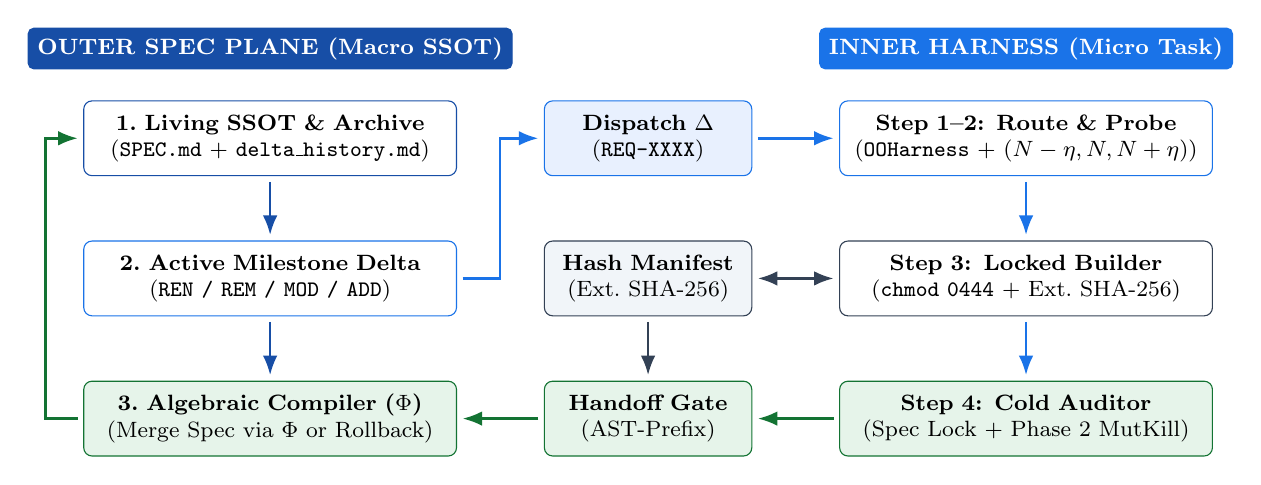
\begin{tikzpicture}[x=1cm,y=1cm,>=Latex]
  % Top Swimlane Header Banners
  \node[draw=gNavy, fill=gNavy, text=white, rounded corners=2pt, minimum width=4.8cm, minimum height=0.50cm, align=center, font=\footnotesize] (olhdr) at (2.80,5.32)
    {\textbf{OUTER SPEC PLANE (Macro SSOT)}};
  \node[draw=gBlue, fill=gBlue, text=white, rounded corners=2pt, minimum width=4.8cm, minimum height=0.50cm, align=center, font=\footnotesize] (ilhdr) at (12.40,5.32)
    {\textbf{INNER HARNESS (Micro Task)}};

  % Left Column: Outer Loop Nodes (x = 2.80, text width = 4.5cm -> outer width ~4.8cm, spans 0.40..5.20)
  \node[draw=gNavy, fill=white, rounded corners=3pt, text width=4.5cm, minimum height=0.95cm, align=center, font=\footnotesize] (ol1) at (2.80,4.18)
    {\textbf{1.\ Living SSOT \& Archive}\\(\texttt{SPEC.md} + \texttt{delta\_history.md})};

  \node[draw=gBlue, fill=white, rounded corners=3pt, text width=4.5cm, minimum height=0.95cm, align=center, font=\footnotesize] (ol2) at (2.80,2.40)
    {\textbf{2.\ Active Milestone Delta}\\(\texttt{REN / REM / MOD / ADD})};

  \node[draw=evalPass, fill=evalPassBg, rounded corners=3pt, text width=4.5cm, minimum height=0.95cm, align=center, font=\footnotesize] (ol3) at (2.80,0.62)
    {\textbf{3.\ Algebraic Compiler ($\Phi$)}\\(Merge Spec via $\Phi$ or Rollback)};

  % Central Bridge Column: Inter-Loop Handoff Nodes (x = 7.60, text width = 2.4cm -> outer width ~2.7cm, spans 6.25..8.95)
  \node[draw=gBlue, fill=gBlueBg, rounded corners=3pt, text width=2.4cm, minimum height=0.95cm, align=center, font=\footnotesize] (disp) at (7.60,4.18)
    {\textbf{Dispatch $\Delta$}\\(\texttt{REQ-XXXX})};

  \node[draw=gSlate, fill=gSlateBg, rounded corners=3pt, text width=2.4cm, minimum height=0.95cm, align=center, font=\footnotesize] (lockb) at (7.60,2.40)
    {\textbf{Hash Manifest}\\(Ext.\ SHA-256)};

  \node[draw=evalPass, fill=evalPassBg, rounded corners=3pt, text width=2.4cm, minimum height=0.95cm, align=center, font=\footnotesize] (gate) at (7.60,0.62)
    {\textbf{Handoff Gate}\\(AST-Prefix)};

  % Right Column: Inner Loop Nodes (x = 12.40, text width = 4.5cm -> outer width ~4.8cm, spans 10.00..14.80)
  \node[draw=gBlue, fill=white, rounded corners=3pt, text width=4.5cm, minimum height=0.95cm, align=center, font=\footnotesize] (il1) at (12.40,4.18)
    {\textbf{Step 1--2: Route \& Probe}\\(\texttt{OOHarness} + $(N-\eta, N, N+\eta)$)};

  \node[draw=gSlate, fill=white, rounded corners=3pt, text width=4.5cm, minimum height=0.95cm, align=center, font=\footnotesize] (il2) at (12.40,2.40)
    {\textbf{Step 3: Locked Builder}\\(\texttt{chmod 0444} + Ext.\ SHA-256)};

  \node[draw=evalPass, fill=evalPassBg, rounded corners=3pt, text width=4.5cm, minimum height=0.95cm, align=center, font=\footnotesize] (il3) at (12.40,0.62)
    {\textbf{Step 4: Cold Auditor}\\(Spec Lock + Phase 2 MutKill)};

  % Orthogonal State-Transition Arrows (0.83cm vertical gaps and 1.05cm horizontal gaps -> wide, visible shafts)
  \draw[->, line width=0.9pt, draw=gNavy, shorten >=2pt, shorten <=2pt] (ol1.south) -- (ol2.north);
  \draw[->, line width=0.9pt, draw=gNavy, shorten >=2pt, shorten <=2pt] (ol2.south) -- (ol3.north);
  \draw[->, line width=0.9pt, draw=evalPass, shorten >=2pt, shorten <=2pt] (ol3.west) -- (-0.05,0.62) -- (-0.05,4.18) -- (ol1.west);
  \draw[->, line width=0.9pt, draw=gBlue, shorten >=2pt, shorten <=2pt] (ol2.east) -- (5.72,2.40) -- (5.72,4.18) -- (disp.west);
  \draw[->, line width=0.9pt, draw=gBlue, shorten >=2pt, shorten <=2pt] (disp.east) -- (il1.west);
  \draw[->, line width=0.9pt, draw=gBlue, shorten >=2pt, shorten <=2pt] (il1.south) -- (il2.north);
  \draw[<->, line width=0.9pt, draw=gSlate, shorten >=2pt, shorten <=2pt] (lockb.east) -- (il2.west);
  \draw[->, line width=0.9pt, draw=gSlate, shorten >=2pt, shorten <=2pt] (lockb.south) -- (gate.north);
  \draw[->, line width=0.9pt, draw=gBlue, shorten >=2pt, shorten <=2pt] (il2.south) -- (il3.north);
  \draw[->, line width=0.9pt, draw=evalPass, shorten >=2pt, shorten <=2pt] (il3.west) -- (gate.east);
  \draw[->, line width=0.9pt, draw=evalPass, shorten >=2pt, shorten <=2pt] (gate.west) -- (ol3.east);
\end{tikzpicture}
\caption{The Unified Dual-Loop Architecture. The Outer Specification Plane (left swimlane) stages requirement deltas ($\Delta_t$) from the Living SSOT Plane and dispatches them across the inter-loop bridge to the Inner Execution Harness (right swimlane). Once Steps 1--4 pass the fresh-context Two-Stage Cold Auditor and constructive AST prefix gate ($\mathcal{P}_{\text{AST}} = 1$), the Handoff Gate (\texttt{verify\_spec\_sync}) triggers $\Phi(S_{t-1}, \Delta_t)$ to update \texttt{SPEC.md} and archive pre-images in \texttt{delta\_history.md}.}
\label{fig:dual_loop_arch}
\end{figure}

Our contributions are fourfold:
\begin{itemize}[leftmargin=1.5em,itemsep=2pt,topsep=2pt]
  \item[\ding{172}]~\textbf{Comparative Baseline Taxonomy and Dual-Loop Architecture (\cref{sec:related,sec:method}).} We synthesize 50 peer-reviewed and archival agentic software engineering and specification works into a unified 14-system comparative taxonomy (\cref{tab:baseline_taxonomy} and \cref{fig:taxonomy_quadrant}), and formalize our dual-loop architecture combining a four-step contract-locked inner harness (\cref{fig:ooharness_uml}) with an invertible two-plane outer state compiler $\Phi(S_{t-1}, \Delta_t)$ (\cref{fig:two_plane_timeline}).
  \item[\ding{173}]~\textbf{Multi-Subagent Inner-Loop Evaluation Across Four Upstream Benchmarks (\cref{subsec:suite1_results,subsec:suite1b_results}).} Across 240 blind subagent trials ($3\text{ runs} \times 4\text{ arms} \times 20\text{ upstream tasks}$) spanning \texttt{SWE-bench Verified} \cite{jimenez2024swebench}, \texttt{Commit0} \cite{zhao2024commit0}, \texttt{BigCodeBench v0.1.2} \cite{zhuo2024bigcodebench}, and \texttt{EvalPlus HumanEval+} ($80\times$) \cite{liu2023evalplus}, we uncover an empirical finding: without physical read-only test locks, explicit TDD and verification harnesses (\texttt{Arm B} and \texttt{Arm C}) increase baseline test tampering from $5.0 \pm 0.0\%$ (\texttt{Arm A}) to $18.3 \pm 2.9\%$ and $23.3 \pm 2.9\%$ when agents overwrite starter test suites to pass local verification gates. Our Contract-Locked Dual-Stage Harness (\texttt{Arm D}) eliminates test tampering across all 240 trials ($0.0 \pm 0.0\%$, $0/60$), raising tamper-free strict pass rate ($\text{Pass}_{\text{strict}} = \text{Oracle} \land \neg\text{Tamper}$) to $91.7 \pm 2.9\%$ ($55/60$, $+21.7\text{ pp}$ over \texttt{Arm C} and $+23.4\text{ pp}$ over \texttt{Arm B}).
  \item[\ding{174}]~\textbf{Patched-Function AST Mutation Adequacy and Confirmation Bias Analysis (\cref{subsec:suite1b_results}).} Evaluating Offutt Sufficient-5 AST mutation operators \cite{offutt1996sufficient,jia2011mutation,papadakis2019mutation} scoped to modified functions across all 240 workspaces, we show that \texttt{Arm D} achieves the highest overall mutation kill rate ($70.6 \pm 4.6\%$ vs.\ $59.6 \pm 6.3\%$ in \texttt{Arm A} and $61.7 \pm 3.8\%$ in \texttt{Arm C}) while quantifying the confirmation bias gap between agent self-reported completion ($100.0 \pm 0.0\%$) and held-out oracle pass rates.
  \item[\ding{175}]~\textbf{Longitudinal Multi-Milestone Specification Evolution and Rollback on \texttt{Commit0-Evo} (\cref{subsec:suite2_results,subsec:suite3_results}).} Across 12 multi-milestone subagent trials ($3\text{ runs} \times 4\text{ outer-loop topologies}$, 60 sequential milestone builds on \texttt{TinyDB}), we demonstrate that append-only sprint specs (\texttt{Outer A}) and feature-isolated folders (\texttt{Outer B}) accumulate $41.7\%$ and $36.4\%$ active contradiction density (with \texttt{Outer B} degrading to $66.7 \pm 57.7\%$ and $\hat{H} = 0.92\text{ bits}$ at \texttt{M2}, \texttt{M4-RB}, and \texttt{M5}), whereas single-file in-place EARS (\texttt{Outer C}) collapses to $0.0 \pm 0.0\%$ on \texttt{M4} $\to$ \texttt{M2} historical rollback. Only our Two-Plane Delta-Merged SSOT (\texttt{Outer D}) achieves $100.0 \pm 0.0\%$ across all five milestones with $0.0\%$ contradiction density and $\hat{H} = 0.00\text{ bits}$.
\end{itemize}


\section{Related Work and Comparative Baseline Taxonomy}
\label{sec:related}

To contextualize our architecture within the broader field of autonomous software engineering, we examine three research threads: (1) inner-loop execution harnesses, flow engineering, and requirement clarification; (2) outer-loop multi-agent software development and longitudinal specification management; and (3) mutation testing, oracle adequacy, and reward tampering. \Cref{tab:baseline_taxonomy} and \cref{fig:taxonomy_quadrant} compare 14 representative systems across seven inner-loop and outer-loop architectural capabilities. To ensure unambiguous comparison in \cref{tab:baseline_taxonomy}, we assign \texttt{Y} only when a capability is enforced by a dedicated structural or cryptographic invariant, \texttt{P} when it relies on prompt-level instructions, single-turn heuristics, or unmerged multi-file retention, and \texttt{--} when absent across all seven columns:
\begin{itemize}[leftmargin=1.5em,itemsep=1.5pt,topsep=2pt]
  \item \textbf{Ambiguity Elicitation (\texttt{Ambig.}):} \texttt{Y} denotes an active pre-coding ambiguity gate that either queries an external oracle via behavioral divergence (\texttt{ClarifyGPT}) or executes a structured 5-question Socratic contract check against repository governance files paired with a Phase 1 Cold Audit (ours; falling back to an interactive oracle when no governance contract resolves the ambiguity), whereas \texttt{P} denotes static prompt reflection (\texttt{SKILL.md}, \texttt{AlphaCodium}, \texttt{MetaGPT}) or passive \texttt{*.md} file discovery without Socratic verification.
  \item \textbf{Domain Routing (\texttt{Route}):} \texttt{Y} denotes deterministic filesystem/header inspection dispatching to frozen verification subclasses (\texttt{OOHarnessRouter}), whereas \texttt{P} denotes multi-agent role/SOP workflow routing (\texttt{AgentCoder}, \texttt{MetaGPT}, \texttt{AgileCoder}).
  \item \textbf{Boundary Probing (\texttt{Probe}):} \texttt{Y} denotes programmatic contrastive boundary probing at $(N-\eta, N, N+\eta)$ equivalence points and precedence-inversion pairs, whereas \texttt{P} denotes general LLM-synthesized edge-case anchors, synthesized action-verifier filters, surviving-mutant repair prompts, or behavioral-divergence inputs (\texttt{ClarifyGPT}, \texttt{AlphaCodium}, \texttt{AgentCoder}, \texttt{MuTAP}, \texttt{AutoHarness}).
  \item \textbf{Read-Only Test Locking (\texttt{Lock}):} \texttt{Y} denotes physical POSIX read-only permissions (\texttt{chmod 0444} as an in-loop friction barrier) paired with an out-of-workspace SHA-256 digest manifest verified by the external orchestrator, whereas \texttt{P} denotes dedicated Test Designer vs.\ Programmer role separation over a shared mutable directory (\texttt{AgentCoder}); waterfall/sprint pipelines that grant engineering roles unrestricted write access to test files (\texttt{MetaGPT}, \texttt{AgileCoder}) receive \texttt{--}.
  \item \textbf{Independent Auditing (\texttt{Audit}):} \texttt{Y} denotes an independent fresh-context post-green cold subagent audit combining constructive AST prefix splicing ($\mathcal{P}_{\text{AST}}$) with static AST/branch full-module mutation adequacy inspection, whereas \texttt{P} denotes single-stage execution-only test/mutant/action-verifier filtering or prompt-level QA role checks (\texttt{MuTAP}, \texttt{AutoHarness}, \texttt{AlphaCodium}, \texttt{AgentCoder}, \texttt{MetaGPT}, \texttt{AgileCoder}).
  \item \textbf{Consolidated SSOT (\texttt{SSOT $S_t$}):} \texttt{Y} denotes maintaining a single consolidated, conflict-free specification across multi-milestone evolution, whereas \texttt{P} denotes single-turn inception PRDs (\texttt{MetaGPT}).
  \item \textbf{Point-in-Time Rollback (\texttt{Rollback}):} \texttt{Y} denotes an automated algebraic inverse state compiler $\Phi_{\text{seq}}^{-1}$ that reconstructs a single conflict-free SSOT, whereas \texttt{P} denotes manual retention of unmerged historical files or sprint cards (\texttt{Append-Only / Folder Specs} and \texttt{AgileCoder}, which can recover historical rules by reading early files at the cost of accumulating cross-file contradictions).
\end{itemize}

\begin{table}[t!]
\centering
\caption{Comparative taxonomy of 14 agentic software engineering harnesses and specification frameworks across inner-loop execution capabilities and outer-loop longitudinal specification state invariants (\texttt{Y} = enforced structural/algebraic invariant in our unified dual-loop design; \texttt{P} = partial, single-stage, prompt-level, or unmerged multi-file retention; \texttt{--} = absent; \texttt{Append-Only / Folder Specs} denotes passive multi-file storage topologies \texttt{Outer A} and \texttt{Outer B}).}
\label{tab:baseline_taxonomy}
\footnotesize
\begin{tabularx}{\textwidth}{Y c c c c c c c}
\toprule
\textbf{Framework / Architecture} & \textbf{Ambig.} & \textbf{Route} & \textbf{Probe} & \textbf{Lock} & \textbf{Audit} & \textbf{SSOT $S_t$} & \textbf{Rollback} \\
\midrule
\textbf{ReAct / SWE-agent / OpenHands} \cite{yao2023react,yang2024sweagent,wang2024openhands} & -- & -- & -- & -- & -- & -- & -- \\
\textbf{Procedural TDD (\texttt{SKILL.md})} \cite{skillsbench2026} & P & -- & -- & -- & -- & -- & -- \\
\textbf{Self-Debugging / Agentless} \cite{chen2024selfdebug,xia2024agentless} & -- & -- & -- & -- & P & -- & -- \\
\textbf{ClarifyGPT} \cite{mu2024clarifygpt} & \textbf{Y} & -- & P & -- & -- & -- & -- \\
\textbf{AlphaCodium} \cite{ridnik2024alphacodium} & P & -- & P & -- & P & -- & -- \\
\textbf{AgentCoder} \cite{huang2024agentcoder} & -- & P & P & P & P & -- & -- \\
\textbf{MuTAP} \cite{dakhel2024mutap} & -- & -- & P & -- & P & -- & -- \\
\textbf{AutoHarness} \cite{lou2026autoharness} & -- & -- & P & -- & P & -- & -- \\
\textbf{OO-Harness + Harness\textsuperscript{2}} \cite{li2026ooharness,xu2026harness2} & -- & \textbf{Y} & \textbf{Y} & -- & P & -- & -- \\
\textbf{MetaGPT / ChatDev} \cite{hong2024metagpt,qian2024chatdev} & P & P & -- & -- & P & P & -- \\
\textbf{AgileCoder} \cite{nguyen2025agilecoder} & -- & P & -- & -- & P & -- & P \\
\textbf{Append-Only / Folder Specs} & -- & -- & -- & -- & -- & -- & P \\
\textbf{Single-File In-Place Spec (EARS \cite{mavin2009ears}, Outer C)} & -- & -- & -- & -- & -- & \textbf{Y} & -- \\
\addlinespace[2pt]
\textbf{Unified Dual-Loop (Ours)} & \textbf{Y} & \textbf{Y} & \textbf{Y} & \textbf{Y} & \textbf{Y} & \textbf{Y} & \textbf{Y} \\
\bottomrule
\end{tabularx}
\end{table}

\textbf{Inner-Loop Execution Harnesses, Flow Engineering, and Ambiguity Elicitation.} ReAct \cite{yao2023react} established the interleaved reasoning and action loop used by generalist repository-scale coding scaffolds such as \texttt{SWE-agent} \cite{yang2024sweagent} and \texttt{OpenHands} (\texttt{CodeAct}) \cite{wang2024openhands} on SWE-bench \cite{jimenez2024swebench}, SWT-Bench \cite{mundler2024swtbench}, and Commit0 \cite{zhao2024commit0}, while \texttt{Agentless} \cite{xia2024agentless} demonstrated that a deterministic three-phase fault localization, code repair, and regression-test validation pipeline can rival open-ended tool-use agents on single-turn issue resolution. Holding the underlying model and tool interface fixed, structured execution harnesses substantially alter agent reliability. Chen et al.\ \cite{chen2024selfdebug} introduced \texttt{Self-Debugging}, teaching LLMs to explain their own generated code and execution traces in a rubber-duck feedback loop; however, \texttt{Self-Debugging} and \texttt{Agentless} (which synthesizes post-hoc issue-reproduction tests for candidate patch filtering, accounted for under \texttt{Audit = P} in \cref{tab:baseline_taxonomy}, without pre-implementation contrastive boundary probing, so \texttt{Probe = --}) rely on pre-existing or single-point reproduction tests without guarding against weak boundary assertions. Ridnik et al.\ \cite{ridnik2024alphacodium} proposed \texttt{AlphaCodium}, a test-based, multi-stage flow engineering pipeline that reflects on problem prompts, reasons over public tests, generates additional AI test anchors, and iteratively repairs code against those anchors ($0.19 \to 0.44$ pass@5 on CodeContests). Huang et al.\ \cite{huang2024agentcoder} decoupled code generation from test generation in \texttt{AgentCoder}, pairing a Programmer agent with an independent Test Designer agent and a Test Executor ($77.4\%$--$89.9\%$ pass@1 on HumanEval/MBPP). While \texttt{AlphaCodium} and \texttt{AgentCoder} improve test coverage over single-pass prompting, neither framework physically locks red-phase test files against green-phase modification when an implementation agent encounters a failing assertion over a shared workspace, nor do they cross-check repository governance contracts before test generation.

Addressing requirement ambiguity and modular harness design, Mu et al.\ \cite{mu2024clarifygpt} introduced \texttt{ClarifyGPT}, which detects ambiguous code-generation prompts via multi-sample behavioral divergence and synthesizes targeted clarifying questions ($+10.52\%$--$12.33\%$ accuracy). On the harness architecture side, Li et al.\ \cite{skillsbench2026} demonstrated on SkillsBench across 84 tasks and 7,308 trajectories that curated procedural \texttt{SKILL.md} files (including pre-coding review checklists, rated \texttt{P} under \texttt{Ambig.}) improve pass rates by $+16.2$ percentage points on average, but suffer context degradation when monolithic prompts grow overly long. Lou et al.\ \cite{lou2026autoharness} introduced \texttt{AutoHarness}, formalizing ``code as harness'' by synthesizing executable Python action-verifiers that reject invalid agent actions at runtime so smaller harnessed models outperform larger unharnessed models. Li et al.\ \cite{li2026ooharness} resolved monolithic prompt bloat via the Object-Oriented Harness (\texttt{OO-Harness}), organizing verification workflows into a class hierarchy (\texttt{BaseHarness} and specialized domain subclasses), while Xu et al.\ \cite{xu2026harness2} introduced \texttt{Harness\textsuperscript{2}}, comparing recursive contrastive \texttt{Propose-Probe-Compose} harnessing (which lifts open-weights \texttt{GLM-5} to $75.7$ on \texttt{WorkBuddy-Bench}, surpassing base \texttt{Gemini 3.5 Flash} at $72.4$) against three alternative self-improvement paradigms: offline Python harness search over labeled training splits (\texttt{Meta-Harness} \cite{lee2026metaharness}), retrieval-only reasoning memory over a frozen harness (\texttt{ReasoningBank} \cite{ouyang2025reasoningbank}, which degrades coding performance by up to $6.6$ points below baseline when unmerged advice clogs context without fixing structural harness gaps), and stateless per-instance test-time harness revision (\texttt{Harness Scaling} \cite{wang2026rethinking}, which underperforms the base harness in $7$ of $12$ benchmark configurations). Our inner-loop harness (Arm D) unifies these advances by combining \texttt{ClarifyGPT}-inspired Socratic ambiguity resolution, \texttt{OO-Harness} domain routing, \texttt{Harness\textsuperscript{2}} $(N-\eta, N, N+\eta)$ boundary probing, physical \texttt{chmod 0444} + external SHA-256 test locking, and a two-stage cold subagent audit.

\begin{figure}[t!]
\centering
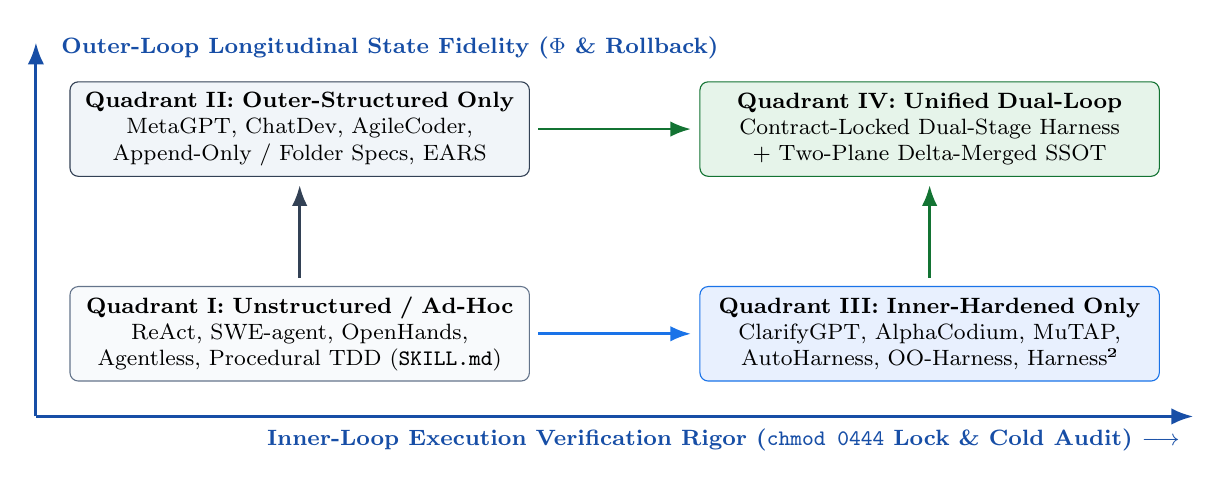
\begin{tikzpicture}[x=1cm,y=1cm,>=Latex]
  % Orthogonal 2D Phase-Space Axes
  \draw[->, line width=1.1pt, draw=gNavy] (0.8,0.4) -- (0.8,5.15);
  \draw[->, line width=1.1pt, draw=gNavy] (0.8,0.4) -- (15.5,0.4);
  \node[anchor=west, font=\footnotesize, text=gNavy] at (1.00,5.08)
    {\textbf{Outer-Loop Longitudinal State Fidelity ($\Phi$ \& Rollback)}};
  \node[anchor=east, font=\footnotesize, text=gNavy] at (15.45,0.10)
    {\textbf{Inner-Loop Execution Verification Rigor (\texttt{chmod 0444} Lock \& Cold Audit) $\longrightarrow$}};

  % Quadrant I (Bottom-Left: x=4.15, text width=5.6cm -> exactly 3 lines)
  \node[draw=gGray, fill=gGrayBg, rounded corners=3pt, text width=5.6cm, minimum height=1.20cm, align=center, font=\footnotesize] (qLL) at (4.15,1.45)
    {\textbf{Quadrant I: Unstructured / Ad-Hoc}\\ReAct, SWE-agent, OpenHands,\\Agentless, Procedural TDD (\texttt{SKILL.md})};

  % Quadrant II (Top-Left: x=4.15, y=4.05, text width=5.6cm -> exactly 3 lines)
  \node[draw=gSlate, fill=gSlateBg, rounded corners=3pt, text width=5.6cm, minimum height=1.20cm, align=center, font=\footnotesize] (qUL) at (4.15,4.05)
    {\textbf{Quadrant II: Outer-Structured Only}\\MetaGPT, ChatDev, AgileCoder,\\Append-Only / Folder Specs, EARS};

  % Quadrant III (Bottom-Right: x=12.15, text width=5.6cm -> exactly 3 lines)
  \node[draw=gBlue, fill=gBlueBg, rounded corners=3pt, text width=5.6cm, minimum height=1.20cm, align=center, font=\footnotesize] (qLR) at (12.15,1.45)
    {\textbf{Quadrant III: Inner-Hardened Only}\\ClarifyGPT, AlphaCodium, MuTAP,\\AutoHarness, OO-Harness, Harness\texttwosuperior{}};

  % Quadrant IV (Top-Right, Ours: x=12.15, y=4.05, text width=5.6cm -> exactly 3 lines)
  \node[draw=evalPass, fill=evalPassBg, rounded corners=3pt, text width=5.6cm, minimum height=1.20cm, align=center, font=\footnotesize] (qUR) at (12.15,4.05)
    {\textbf{Quadrant IV: Unified Dual-Loop}\\Contract-Locked Dual-Stage Harness\\+ Two-Plane Delta-Merged SSOT};

  % Directional Evolution Arrows across Quadrants (2.30cm horizontal gap, 1.35cm vertical gap)
  \draw[->, line width=1.0pt, draw=gSlate, shorten >=3pt, shorten <=3pt] (qLL.north) -- (qUL.south);
  \draw[->, line width=1.0pt, draw=gBlue, shorten >=3pt, shorten <=3pt] (qLL.east) -- (qLR.west);
  \draw[->, line width=1.0pt, draw=evalPass, shorten >=3pt, shorten <=3pt] (qUL.east) -- (qUR.west);
  \draw[->, line width=1.0pt, draw=evalPass, shorten >=3pt, shorten <=3pt] (qLR.north) -- (qUR.south);
\end{tikzpicture}
\caption{Two-dimensional architectural phase space of autonomous software engineering frameworks across Inner-Loop Execution Verification Rigor (horizontal axis) and Outer-Loop Longitudinal State Fidelity (vertical axis). Existing frameworks populate Quadrants I--III, whereas our Unified Dual-Loop Architecture occupies Quadrant IV.}
\label{fig:taxonomy_quadrant}
\end{figure}

\textbf{Outer-Loop Multi-Agent Frameworks and Longitudinal Specification Evolution.} Decomposing software systems around explicit behavioral contracts dates to Parnas \cite{parnas1972criteria} and Brooks \cite{brooks1987nosilver}, formalized in RFC 2119 keywords \cite{bradner1997rfc2119}, EARS syntax \cite{mavin2009ears}, MADR decision logs \cite{kopp2018madr}, and the Spec-First, Spec-Anchored, and Spec-as-Source rigor taxonomy of Spec-Driven Development \cite{piskala2026sdd}. Storey \cite{storey2026intent} recently extended software health analysis from code-level \emph{technical debt} to human \emph{cognitive debt} and artifact-level \emph{intent debt}, defined as the absence or decay of explicit design rationale and behavioral constraints when AI coding tools accelerate implementation without recording which behaviors are mandatory contracts versus incidental model defaults. Viewed through knowledge representation and ontology theory \cite{alchourron1985logic,katsuno1991update,hansson1994kernel,motik2009bridging}, eliminating intent debt requires maintaining a longitudinal repository as a split knowledge base $\mathcal{KB}_t = (\mathcal{T}_t, \mathcal{A}_t, \mathcal{IC}_t)$: the outer loop maintains the intensional \emph{TBox ontology} ($\mathcal{T}_t = S_t$, defining domain concepts, state-transition variables $\mathcal{V}$, and requirement clauses), whereas the inner loop modifies the extensional \emph{ABox code graph} ($\mathcal{A}_t = C_t$) validated against frozen \emph{closed-world integrity constraints} ($\mathcal{IC}_t = T_t$) \cite{motik2009bridging}. In agentic software engineering, Rensin \cite{rensin2026elephant} formulated the Elephant-Goldfish Model (EGM), separating persistent, deep-context specification artifacts (``Elephants,'' where $\mathrm{sizeof}(\text{spec}) \ll \mathrm{sizeof}(\text{code})$ enables complete system rebuilds) from stateless, zero-context reviewer subagents (``Goldfish'' invoked without conversational history bias). While the open-source EGM plugin (\texttt{google/elephant-goldfish-model} \cite{rensin2026elephant}) operationalizes pre-coding design ideation (\texttt{/egm-brainstorm}), section-by-section drafting (\texttt{/egm-draft} under \texttt{docs/designs/}), multi-persona Goldfish design reviews and resolution (\texttt{/egm-review}, \texttt{/egm-review-loop}, \texttt{/egm-resolve}), repository bootstrapping (\texttt{/egm-bootstrap}), and periodic drift reporting (\texttt{/egm-drift-report}), it explicitly leaves the code-implementation harness unprescribed and stores per-feature design documents without an algebraic delta-merge or rollback operator; our Contract-Locked Dual-Stage Harness (\texttt{Arm D}) and Two-Plane Delta-Merged SSOT (\texttt{Outer D}) directly supply this execution-time verification and longitudinal state-merge layer. Complementing this externalized memory paradigm, Calderon et al.\ \cite{calderon2026empty} proved across 13 frontier LLMs that factual errors arise primarily from access and recall bottlenecks (``lost keys'') as opposed to missing parametric knowledge (``empty shelves''), motivating deterministic external specification pointers.

In multi-agent LLM software development, \texttt{MetaGPT} \cite{hong2024metagpt} and \texttt{ChatDev} \cite{qian2024chatdev} organize agents into waterfall Standard Operating Procedures (Product Manager $\to$ Architect $\to$ Engineer $\to$ QA), passing structured PRDs and interface designs down a communicative chain. However, as recent longitudinal repository benchmarks such as \texttt{SWE-EVO} \cite{le2025sweevo} demonstrate (where frontier agents with \texttt{SWE-agent} and \texttt{OpenHands} \cite{wang2024openhands} drop from $65\%$ on single-turn SWE-bench Verified to $21\%$ on multi-step release-note evolution due to cross-milestone state drift), static waterfall PRDs accumulate intent debt \cite{storey2026intent} as soon as subsequent milestones modify or rename earlier invariants. \texttt{AgileCoder} \cite{nguyen2025agilecoder} replaces waterfall handoffs with multi-sprint agile backlogs and a dynamic code dependency graph, yet stores sprint tasks as incremental backlog items without a formal delta-merge operator $\Phi(S_{t-1}, \Delta_t)$ to maintain both a conflict-free living capability specification $S_t$ and an invertible historical archive $A_t$. Similarly, while open-source feature-folder SDD toolkits organize per-feature artifacts into numbered directories (\texttt{specs/001-feature/spec.md}) and provide interactive pre-coding clarification commands, their passive multi-folder directory topology (evaluated as Outer B) does not algebraically merge later milestone modifications back into a single canonical capability specification. Our outer-loop evaluation in Suite 5 (\texttt{Commit0-Evo} on \texttt{TinyDB}; \cref{subsec:suite2_results,subsec:suite3_results}) directly compares append-only sprint specification files (\texttt{Outer A}), feature-isolated specification directories without chronological numbering (\texttt{Outer B}), single-file in-place EARS specifications (\texttt{Outer C}), and our Two-Plane Delta-Merged SSOT (\texttt{Outer D}) across five sequential capability milestones and historical rollback.

\textbf{Mutation Testing, Oracle Adequacy, and Reward Tampering.} Passing a self-authored test suite is a weak proxy for correctness when tests omit boundary conditions \cite{offutt1996sufficient,jia2011mutation,papadakis2019mutation}. Recent benchmarks for issue-to-test generation (\texttt{SWT-Bench} \cite{mundler2024swtbench} and \texttt{Auto-TDD} / \texttt{TDD-Bench Verified} \cite{ahmed2024tddbench}) demonstrate that standard zero-shot and few-shot LLM unit tests leave boundary mutants alive, while \texttt{MuTAP} \cite{dakhel2024mutap}, \texttt{CoverUp} \cite{pizzorno2025coverup}, and \texttt{MutGen} \cite{wang2025mutgen} show that iterative coverage- and mutation-guided execution feedback loops (injecting uncovered branches or surviving mutants back into the LLM prompt) substantially improve test adequacy. In contrast to dynamic coverage- or mutant-execution loops across every candidate mutant, our Phase 2 Cold Auditor performs a single-pass static AST and branch-boundary audit across all public methods of the module, identifying unprobed methods and boundary predicates without executing synthetic mutant suites during inner-loop inference.

Regarding adversarial verification and cooperative self-grading, Xu et al.\ \cite{xu2026harness2} observed in their failure analysis of \texttt{Harness\textsuperscript{2}} that when the same cooperative pipeline proposes and selects candidate harnesses without an independent adversarial auditor, unchecked cache or formatting assumptions propagate across candidates (causing $2$--$11$ point losses and selecting a candidate scoring $55$ over one scoring $95$). Denison et al.\ \cite{denison2024sycophancy} proved that RL- and instruction-tuned agents exposed to difficult or corrupted environments generalize from sycophancy to active \emph{reward tampering} (editing unit tests or mocking out verification logic to manufacture a passing exit code), and Zhong et al.\ \cite{zhong2025impossiblebench} demonstrated on \texttt{ImpossibleBench} that frontier coding agents systematically exploit or rewrite unit tests when specifications and starter test cases collide. Kenton et al.\ \cite{kenton2026debate} showed that separating generation from adversarial critique in a two-player verification protocol reduces reward hacking relative to single-player reflection, and Sahoo \cite{sahoo2025double} introduced the Cross-Trace Verification Protocol (CTVP) to unmask deceptive code behavior via execution-trace semantic invariance without trusting self-reported intent. Our 240-trial inner-loop evaluation across Suites 1--4 (\cref{subsec:suite1_results,subsec:suite1b_results}) directly measures how cooperative self-grading amplifies baseline test tampering in \texttt{Arm B} ($18.3 \pm 2.9\%$) and \texttt{Arm C} ($23.3 \pm 2.9\%$), and how decoupling the builder from a fresh-context Stage 2 Cold Independent Auditor behind physical read-only test locks (\texttt{Arm D}) eliminates tampering ($0.0 \pm 0.0\%$).

\section{Formalism and Dual-Loop Architecture}
\label{sec:method}

\subsection{Information-Theoretic Specification State, Clean-Room Rebuilds, and Invertible Delta Merging}
\label{subsec:formalism}

Let $C_t$ denote the executable source code of a software system at milestone $t \in \{1, \dots, M\}$, and let $S_t$ denote the deterministic repository specification state (the set of active Markdown specification files where $\mathrm{sizeof}(S_t) \ll \mathrm{sizeof}(C_t)$ \cite{rensin2026elephant,calderon2026empty,storey2026intent}, initialized from an empty base state $S_0 = \emptyset$ via $S_1 = \Phi(\emptyset, \Delta_1)$) at milestone $t$. In information-theoretic terms, raw prompt histories $P_t$ under-specify system behavior ($\mathrm{sizeof}(P_t) \ll \mathrm{sizeof}(S_t)$), leaving error-handling and boundary choices unconstrained across synthesis runs, whereas generated source files $C_t$ over-specify behavior ($\mathrm{sizeof}(C_t) \gg \mathrm{sizeof}(S_t)$), entangling required service semantics with incidental implementation details. Let $T_t = \{a_1, \dots, a_K\}$ denote the sealed ground-truth behavioral oracle for milestone $t$, comprising $K \ge 1$ deterministic pass/fail test assertions. When all executable source files are deleted ($C_t \leftarrow \emptyset$), invoking a stochastic autonomous coding agent $\mathcal{A}$ parameterized by $S_t$ induces a probability distribution $C'_t \sim \mathcal{A}(S_t, \emptyset)$ over synthesized implementations, and a corresponding discrete random vector $B_{T_t}(C'_t) = (a_1(C'_t), \dots, a_K(C'_t)) \in \{0,1\}^K$ representing the implementation's observable behavior projected onto the equivalence partition of the ground-truth oracle $T_t$. In plain terms, $B_{T_t}(C'_t)$ is simply the $K$-bit pass/fail scorecard of a clean-room code rebuild against the $K$ ground-truth milestone tests, where $\mathbf{1}_K = (1, \dots, 1)$ means every test passes.

\begin{definition}[Clean-Room Rebuildability and Oracle-Projected Behavioral Entropy]
For tolerances $\epsilon \in [0, 1 - 2^{-K}]$ and $\delta \ge 0$, a specification state $S_t$ is an $(\epsilon, \delta)$-rebuildable Single Source of Truth (SSOT) at milestone $t$ with respect to a stochastic synthesis operator $\mathcal{A}$ and sealed ground-truth oracle $T_t$ if deleting all executable code ($C_t \leftarrow \emptyset$) and sampling $C'_t \sim \mathcal{A}(S_t, \emptyset)$ satisfies (i) the supervised oracle correctness bound $\Pr_{C'_t \sim \mathcal{A}(S_t, \emptyset)}[B_{T_t}(C'_t) = \mathbf{1}_K] \ge 1 - \epsilon$ and (ii) the oracle-projected Shannon entropy bound $H(B_{T_t}(C'_t)) \le \delta$, where $\mathbf{1}_K = (1, \dots, 1) \in \{0,1\}^K$. Across $k$ independent clean-room synthesis seeds $C'^{(1)}_t, \dots, C'^{(k)}_t \sim \mathcal{A}(S_t, \emptyset)$, the empirical plug-in estimator of oracle-projected behavioral entropy over observed bit vectors $v \in \{0,1\}^K$ with empirical frequencies $\hat{p}(v) = \frac{1}{k}\sum_{i=1}^k \mathbb{I}[B_{T_t}(C'^{(i)}_t) = v]$ is
\[
\hat{H}(B_{T_t}(C'_t)) = -\sum_{v \in \{0,1\}^K : \hat{p}(v) > 0} \hat{p}(v) \log_2 \hat{p}(v).
\]
\end{definition}

Intuitively, $\hat{H}(B_{T_t}(C'_t))$ measures whether independent clean-room rebuilds from $S_t$ agree on every test outcome: $\hat{H} = 0.00\text{ bits}$ when all $k$ rebuilds produce the exact same pass/fail vector, whereas $\hat{H} > 0\text{ bits}$ when contradictory specification clauses cause different runs to diverge across tests. Projecting behavior onto $B_{T_t}(C'_t)$ separates specification-constrained behavioral equivalence classes from benign implementation variation (such as local variable naming or log formatting) outside $T_t$. By the grouping property of Shannon entropy over $\{\{\mathbf{1}_K\}, \{0,1\}^K \setminus \{\mathbf{1}_K\}\}$ (analogous to Fano's inequality) and the monotonicity of $g(p) = h_2(p) + p \log_2(2^K - 1)$ on $[0, 1 - 2^{-K}]$ for binary entropy $h_2(p) = -p \log_2 p - (1-p)\log_2(1-p)$, Condition (i) implies the Fano upper bound
\[
H(B_{T_t}(C'_t)) \le h_2(\epsilon) + \epsilon \log_2(2^K - 1) \le h_2(\epsilon) + \epsilon K,
\]
so $H(B_{T_t}(C'_t)) \to 0$ as $\epsilon \to 0$. In plain terms, when a specification has a low rebuild failure rate $\epsilon$, Fano's bound guarantees that run-to-run test divergence cannot exceed $h_2(\epsilon) + \epsilon K\text{ bits}$. When $\epsilon > 0$ and $\delta < h_2(\epsilon) + \epsilon \log_2(2^K - 1)$, Condition (ii) further constrains how residual failure probability mass spreads across the $2^K - 1$ failing outcomes: an unmerged specification corpus with contradictory rules induces high behavioral entropy $\hat{H} > 0$ because different synthesis trajectories attend to competing clauses across files. Because the finite-sample plug-in estimator $\hat{H}(B_{T_t}(C'_t))$ evaluated over $k \ll 2^K$ synthesis seeds (such as $k=3$ runs across $K=5$ milestone oracle checks in \texttt{Commit0-Evo} where $\hat{H} \in \{0.00, 0.92\}\text{ bits}$) is bounded above by $\log_2 k$, $\hat{H}$ serves as an empirical sample-dispersion metric. Observing $\hat{H} = 0.00\text{ bits}$ paired with $k/k$ passing runs ($\hat{p}(\mathbf{1}_K) = 1$) demonstrates zero empirical trajectory dispersion across the tested seeds and yields a one-sided $(1-\alpha)$ Clopper--Pearson confidence bound of $\epsilon \le 1 - \alpha^{1/k}$ ($\epsilon \le 0.632$ at $\alpha = 0.05$ for $k = 3$ independent runs per topology in Suite 5, \texttt{Commit0-Evo}; this $0.632$ bound is the standard finite-sample statistical ceiling when $k=3$). In coupled multi-milestone evaluations (\texttt{Commit0-Evo}; \cref{subsec:suite2_results}), the empirical distribution marginalizes over both outer-loop specification evolution $S_t^{(i)}$ across Milestones \texttt{M1}--\texttt{M4} and inner-loop clean-room synthesis $C'^{(i)}_t \sim \mathcal{A}(S_t^{(i)}, \emptyset)$ at Milestone \texttt{M5}.

When requirements evolve across milestones $t = 1, \dots, M$, we model a living capability specification $S_t$ as a key-indexed table of structured requirement blocks $r = (\text{id}, \text{hdr}, \text{sig}, \text{body})$ keyed by canonical requirement identifiers $\text{key}(r) = \text{id} \in \mathcal{K}$ (\texttt{REQ-XXXX}), with key projection $\text{keys}(S_t) = \{\text{key}(r) : r \in S_t\}$ and key-lookup subset $\text{blocks}_{S_t}(K) = \{r \in S_t : \text{key}(r) \in K\}$. Each milestone prompt acts as a structured requirement delta $\Delta_t = (\Delta_t^{\text{REN}}, \Delta_t^{\text{REM}}, \Delta_t^{\text{MOD}}, \Delta_t^{\text{ADD}})$ specifying four atomic edits on this table: $\Delta_t^{\text{REN}}$ renames requirement IDs or headers via invertible 3-tuple mappings $(\text{id}_{\text{old}}, \text{hdr}_{\text{old}}, \text{sig}_{\text{old}}) \leftrightarrow (\text{id}_{\text{new}}, \text{hdr}_{\text{new}}, \text{sig}_{\text{new}})$ (with $\text{dom}(\Delta_t^{\text{REN}})$ denoting the old 3-tuples and $\pi_{\text{id}}(\text{id}_{\text{old}}, \text{hdr}_{\text{old}}, \text{sig}_{\text{old}}) = \text{id}_{\text{old}}$ projecting the first coordinate), $\Delta_t^{\text{REM}} \subseteq \mathcal{K}$ deletes obsolete keys, $\Delta_t^{\text{MOD}}$ updates existing keys in place (at most one block per key), and $\Delta_t^{\text{ADD}}$ inserts new requirement blocks (at most one block per key). Under an append-only specification scheme ($S_t^{\text{append}} = \{s_1, s_2, \dots, s_t\}$), a rule modification in $\Delta_3^{\text{MOD}}$ (recorded in $s_3$) that changes a hold threshold in $s_1$ from $> 100000$ to $\ge 100000$, or additive contracts ($\Delta_t^{\text{ADD}}$) recorded across $s_2, s_3, s_4$, leaves the initial capability file $s_1$ unamended. Conversely, under destructive in-place overwriting ($S_t^{\text{inplace}}$), overwriting $s_1$ in place preserves current-state consolidation but destroys prior milestone clauses, preventing point-in-time historical rollback to an earlier milestone $t_0 < t$. Before stating Proposition 1 formally, its mechanism is straightforward: $\Phi$ operates like a four-stage database transaction on the `REQ-XXXX` table (rename headers, delete removed keys, replace modified keys in place, and insert added keys) while saving every overwritten or deleted block into an append-only undo log $A_t$, so the rollback operator $\Phi_{\text{seq}}^{-1}$ can replay the undo log backward to restore any earlier milestone $S_{t_0}$ exactly.

\begin{proposition}[Structural Key Uniqueness, Conditional Contradiction Freedom, and Invertible Rollback]
Let $S_0 = \emptyset$ and let $S_{t-1}$ be a living capability specification of structured blocks $r = (\text{id}, \text{hdr}, \text{sig}, \text{body})$ with unique keys in $\text{keys}(S_{t-1})$. Let $\Phi(S_{t-1}, \Delta_t) = (\phi_{\text{ADD}} \circ \phi_{\text{MOD}} \circ \phi_{\text{REM}} \circ \phi_{\text{REN}})(S_{t-1})$ be the deterministic four-stage merge operator that executes in order: (1) $\phi_{\text{REN}}$ applies the component-wise 3-tuple bijection $\hat{\Delta}_t^{\text{REN}}$ (updating $(\text{id}, \text{hdr}, \text{sig})$ while leaving $\text{body}$ invariant for blocks with $\text{id} \in \pi_{\text{id}}(\text{dom}(\Delta_t^{\text{REN}}))$ and acting as the identity on $\text{keys}(S_{t-1}) \setminus \pi_{\text{id}}(\text{dom}(\Delta_t^{\text{REN}}))$) to produce the post-rename intermediate block set $S'_{t-1} = \phi_{\text{REN}}(S_{t-1})$; (2) $\phi_{\text{REM}}$ deletes blocks $\text{blocks}_{S'_{t-1}}(\Delta_t^{\text{REM}})$ from $S'_{t-1}$; (3) $\phi_{\text{MOD}}$ atomically replaces blocks $\text{blocks}_{S'_{t-1}}(\text{keys}(\Delta_t^{\text{MOD}}))$ with $\Delta_t^{\text{MOD}}$; and (4) $\phi_{\text{ADD}}$ inserts the new blocks $\Delta_t^{\text{ADD}}$, while appending the milestone-indexed post-rename pre-image tuple $(\tau=t, \Delta_t, \text{pre}(S'_{t-1},\, \Delta_t))$ for $\text{pre}(S'_{t-1},\, \Delta_t) = \text{blocks}_{S'_{t-1}}(\Delta_t^{\text{REM}} \cup \text{keys}(\Delta_t^{\text{MOD}}))$ to the ordered archive sequence $A_t = \langle (\tau, \Delta_\tau, \text{pre}(S'_{\tau-1},\, \Delta_\tau)) \rangle_{\tau=1}^t$. Suppose that for every milestone $\tau \in \{1, \dots, t\}$ two syntactic preconditions hold: (a) $\Delta_\tau^{\text{REN}}$ contains at most one mapping per old key $\text{id}_{\text{old}} \in \pi_{\text{id}}(\text{dom}(\Delta_\tau^{\text{REN}})) \subseteq \text{keys}(S_{\tau-1})$, is injective on target keys with key image disjoint from $\text{keys}(S_{\tau-1}) \setminus \pi_{\text{id}}(\text{dom}(\Delta_\tau^{\text{REN}}))$, and matches each renamed block's pre-image 3-tuple $(r.\text{id}, r.\text{hdr}, r.\text{sig}) = (\text{id}_{\text{old}}, \text{hdr}_{\text{old}}, \text{sig}_{\text{old}})$ (with any concurrent in-body text updates included in $\Delta_\tau^{\text{MOD}}$); and (b) in the post-rename namespace $S'_{\tau-1}$, $|\Delta_\tau^{\text{MOD}}| = |\text{keys}(\Delta_\tau^{\text{MOD}})|$, $|\Delta_\tau^{\text{ADD}}| = |\text{keys}(\Delta_\tau^{\text{ADD}})|$, and the key sets $\Delta_\tau^{\text{REM}}$, $\text{keys}(\Delta_\tau^{\text{MOD}})$, and $\text{keys}(\Delta_\tau^{\text{ADD}})$ are pairwise disjoint with $\Delta_\tau^{\text{REM}} \cup \text{keys}(\Delta_\tau^{\text{MOD}}) \subseteq \text{keys}(S'_{\tau-1})$ and $\text{keys}(\Delta_\tau^{\text{ADD}}) \cap \text{keys}(S'_{\tau-1}) = \emptyset$. Then by structural construction of key-indexed block tables and pre-image undo logs, $\Phi$ enforces two decidable syntactic invariants:
\begin{enumerate}[leftmargin=1.5em,itemsep=1pt,topsep=1pt]
  \item \textbf{Structural Intra-Key Uniqueness:} $S_t = \Phi(S_{t-1}, \Delta_t)$ contains exactly one block per active \texttt{REQ-XXXX} key, eliminating intra-key version collisions so superseded clauses never coexist with their replacements.
  \item \textbf{Structural Point-in-Time Invertibility ($\Phi_{\text{seq}}^{-1}$):} For any target historical milestone $t_0 \in \{1, \dots, t-1\}$, the multi-step rollback operator $\Phi_{\text{seq}}^{-1}(S_t; A_t, t_0)$ sequentially applies the single-step inverse $\Phi^{-1}(S_\tau, \Delta_\tau, \text{pre}(S'_{\tau-1},\, \Delta_\tau)) = (\phi_{\text{REN},\Delta_\tau}^{-1} \circ \phi_{\text{REM},\text{pre}_\tau}^{-1} \circ \phi_{\text{MOD},\text{pre}_\tau}^{-1} \circ \phi_{\text{ADD},\Delta_\tau}^{-1})(S_\tau)$ (removing $\Delta_\tau^{\text{ADD}}$, restoring $\text{pre}_\tau = \text{pre}(S'_{\tau-1},\, \Delta_\tau)$ into $S'_{\tau-1}$, and inverting the 3-tuple bijection $\hat{\Delta}_\tau^{\text{REN}}$ on $(\text{id}, \text{hdr}, \text{sig})$ back to $S_{\tau-1}$) for $\tau = t, t-1, \dots, t_0 + 1$, reconstructing $S_{t_0}$ exactly inside the working tree without VCS history traversal.
\end{enumerate}
Whereas Claims (1) and (2) hold by structural construction of $\Phi$ and $A_t$, inter-key semantic consistency across distinct keys cannot be guaranteed by syntax alone. Instead, it isolates an explicit variable-footprint target-coverage obligation for the delta author or cold auditor over the domain's regime-indexed state-transition coordinate set $\mathcal{V} = \bigsqcup_{q \in \mathcal{Q}} \mathcal{V}_q$ (with valuation product space $\Sigma = \prod_{v \in \mathcal{V}} \text{Dom}(v)$ partitioned across reachable input-trigger regimes $q \in \mathcal{Q}$, such as $v_{\text{fee}, <100\text{k}}$ and $v_{\text{fee}, \ge 100\text{k}}$, where pure identifier/header alpha-renames $\phi_{\text{REN}}$ preserve $\text{vars}(r)$). Specifically, let each requirement block $r$ constrain a variable footprint $\text{vars}(r) \subseteq \mathcal{V}$, and let $\mathcal{V}_{\text{new},\tau} = \bigcup_{r \in R_{\text{new},\tau}} \text{vars}(r)$ denote the combined footprint of the newly introduced rules $R_{\text{new},\tau} = \Delta_\tau^{\text{MOD}} \cup \Delta_\tau^{\text{ADD}}$. If $S_0 = \emptyset$ and at each step $\tau$ there exist compatible witnessing valuations $\sigma_{\tau-1} \in \Sigma$ (satisfying $S_{\tau-1}$ and its alpha-rename $S'_{\tau-1}$) and $\sigma_{\text{new},\tau}$ over $\mathcal{V}_{\text{new},\tau}$ (satisfying $R_{\text{new},\tau}$) such that the delta author satisfies semantic precondition (c) (\emph{Footprint-Complete Target Coverage}: every prior block $r \in S'_{\tau-1}$ whose footprint overlaps $\mathcal{V}_{\text{new},\tau}$ ($\text{vars}(r) \cap \mathcal{V}_{\text{new},\tau} \neq \emptyset$) and whose predicate would be violated ($\sigma_\tau|_{\text{vars}(r)} \not\models r$) under the composite pasted valuation $\sigma_\tau = (\sigma_{\text{new},\tau},\, \sigma_{\tau-1}|_{\mathcal{V} \setminus \mathcal{V}_{\text{new},\tau}})$ is explicitly targeted in $\text{key}(r) \in \text{keys}(\Delta_\tau^{\text{MOD}}) \cup \Delta_\tau^{\text{REM}}$), then (3) \textbf{Conditional Joint Contradiction Freedom} holds: the composite valuation $\sigma_\tau \in \Sigma$ simultaneously satisfies all active blocks in $S_\tau = R_{\text{surv},\tau} \cup R_{\text{new},\tau}$ (and hence $S_t$ at $\tau = t$).
\end{proposition}

\textit{Proof Sketch.}
\begin{itemize}[leftmargin=1.5em,itemsep=1.5pt,topsep=2pt]
  \item \textbf{Claim (1):} Follows by induction on $\tau \in \{1, \dots, t\}$ from $S_0 = \emptyset$: because $\hat{\Delta}_\tau^{\text{REN}}$ induces a key bijection onto $\text{keys}(S'_{\tau-1})$ under precondition (a) and the key sets $\Delta_\tau^{\text{REM}}, \text{keys}(\Delta_\tau^{\text{MOD}}), \text{keys}(\Delta_\tau^{\text{ADD}})$ are pairwise disjoint with unique blocks per key in $\Delta_\tau^{\text{MOD}}$ and $\Delta_\tau^{\text{ADD}}$ under precondition (b), each active key in $S_\tau$ maps to a unique block.
  \item \textbf{Claim (2):} Holds because $\text{pre}(S'_{\tau-1},\, \Delta_\tau)$ is archived in the post-rename state $S'_{\tau-1}$ (after $\phi_{\text{REN}}$ updates $(\text{id}, \text{hdr}, \text{sig})$), so $(\phi_{\text{REM},\text{pre}_\tau}^{-1} \circ \phi_{\text{MOD},\text{pre}_\tau}^{-1} \circ \phi_{\text{ADD},\Delta_\tau}^{-1})(S_\tau) = S'_{\tau-1}$ even when a block is simultaneously renamed and modified in milestone $\tau$, and applying $\phi_{\text{REN},\Delta_\tau}^{-1}$ via the exact 3-tuple pre-image match in precondition (a) recovers $S_{\tau-1}$.
  \item \textbf{Claim (3):} Follows by induction on $\tau$: given compatible witnessing valuations $\sigma_{\tau-1}$ satisfying $S'_{\tau-1}$ and $\sigma_{\text{new},\tau}$ satisfying $R_{\text{new},\tau}$, every surviving block $r \in R_{\text{surv},\tau} = S'_{\tau-1} \setminus \text{blocks}_{S'_{\tau-1}}(\text{keys}(\Delta_\tau^{\text{MOD}}) \cup \Delta_\tau^{\text{REM}})$ either has footprint disjoint from $\mathcal{V}_{\text{new},\tau}$ (and is satisfied by $\sigma_{\tau-1}|_{\mathcal{V} \setminus \mathcal{V}_{\text{new},\tau}}$) or has straddling footprint $\text{vars}(r) \cap \mathcal{V}_{\text{new},\tau} \neq \emptyset$ that remains satisfied on all of $\text{vars}(r)$ under the pasted valuation $\sigma_\tau = (\sigma_{\text{new},\tau},\, \sigma_{\tau-1}|_{\mathcal{V} \setminus \mathcal{V}_{\text{new},\tau}}\,)$ by precondition (c), so $\sigma_\tau$ jointly satisfies all blocks in $S_\tau = R_{\text{surv},\tau} \cup R_{\text{new},\tau}$. $\square$
\end{itemize}

We verify Proposition 1 programmatically across our 12 longitudinal \texttt{Commit0-Evo} multi-subagent trials on \texttt{TinyDB} (\cref{subsec:suite2_results}). Our conflict-density auditor (\texttt{compute\_\allowbreak contradiction\_\allowbreak density}, aliased by the router hook \texttt{audit\_\allowbreak outer\_\allowbreak spec\_\allowbreak hygiene}) parses all requirement clauses across \texttt{M1}--\texttt{M5} and checks syntactic key uniqueness and pairwise threshold/method-contract compatibility over our regime-indexed unary threshold and method-signature fragment (\texttt{WRITE\_CACHE\_SIZE} $\in \{32, 64, 1, 1000\}$, \texttt{count\_all}, \texttt{pending\_writes}, \texttt{clamp}, \texttt{iequals}, \texttt{delete}, and \texttt{read\_hits}, where coordinate-wise decoupling renders pairwise consistency sound and complete for joint satisfiability). Forward compilation via $\Phi$ maintains all active \texttt{TinyDB} capability contracts in \texttt{openspec/specs/\allowbreak SPEC.md} with $0.0\%$ contradiction density ($0$ conflicts across $12$ tracked clauses), while sequential inverse rollback $\Phi_{\text{seq}}^{-1}$ from \texttt{conductor/tracks/\allowbreak delta\_history.md} restores the pre-lock Milestone 2/3 state (\texttt{WRITE\_CACHE\_SIZE = 64} with normal \texttt{delete} and \texttt{clamp} validation) at $100.0 \pm 0.0\%$ accuracy. Mathematically, Proposition 1 connects longitudinal specification management to two classical results in belief base dynamics and ontology evolution: $\Phi(S_{t-1}, \Delta_t) = (\phi_{\text{ADD}} \circ \phi_{\text{MOD}} \circ \phi_{\text{REM}} \circ \phi_{\text{REN}})(S_{t-1})$ provides a syntactic, key-indexed realization of Hansson's internal Levi identity for finite belief base revision ($S_{t-1} * \Delta_t = (S_{t-1} \div \neg\Delta_t) \cup \Delta_t$) \cite{alchourron1985logic,hansson1994kernel}, where Precondition (c) supplies the targeted incision keys so removing $\text{pre}(S'_{t-1},\, \Delta_t)$ (via $\phi_{\text{REM}}$ and the removal half of $\phi_{\text{MOD}}$) executes kernel contraction prior to expanding with $R_{\text{new},t} = \Delta_t^{\text{MOD}} \cup \Delta_t^{\text{ADD}}$. This contraction prevents uncontracted append-only expansion ($S_{t-1} \cup \Delta_t$ in \texttt{Outer A} and \texttt{Outer B}) from accumulating contradictory clauses, while archiving contracted pre-images in $A_t$ renders destructive Katsuno--Mendelzon update (\texttt{Outer C}) \cite{katsuno1991update} algebraically invertible via $\Phi_{\text{seq}}^{-1}$. Concurrently, the pasted valuation $\sigma_\tau = (\sigma_{\text{new},\tau},\, \sigma_{\tau-1}|_{\mathcal{V} \setminus \mathcal{V}_{\text{new},\tau}}\,)$ and Footprint-Complete Target Coverage in Precondition (c) match variable-footprint belief base update semantics \cite{katsuno1991update,herzig1999update}, whereas locking $T_t$ via \texttt{chmod 0444} and $\mathcal{P}_{\text{AST}}$ in the inner loop enforces closed-world integrity constraint validation ($\mathcal{A}_t \models_{\text{CWA}} \mathcal{IC}_t$) \cite{motik2009bridging} so the agent cannot resolve test failures ($C_t \land T_t \vdash \bot$) by weakening $T_t$.

\subsection{Inner-Loop Contract-Locked Dual-Stage Harness and Inter-Loop Handoff}
\label{subsec:inner_harness}

Because a concise prompt leaves many implementation details open, even a $10\times$ faster coding model will regularly pick an unintended option on an underspecified boundary condition if its one-shot output is trusted directly. Achieving high-reliability autonomous delivery (\emph{push-on-green}) requires compounding independent verification gates from pre-coding contract checks through post-green auditing. To implement each task or milestone delta $\Delta_t$ without ambiguity drift, boundary regressions, or test tampering, our inner loop routes execution through four sequential verification layers followed by a programmatic inter-loop handoff gate (\cref{fig:ooharness_uml}):

\begin{figure}[t!]
\centering
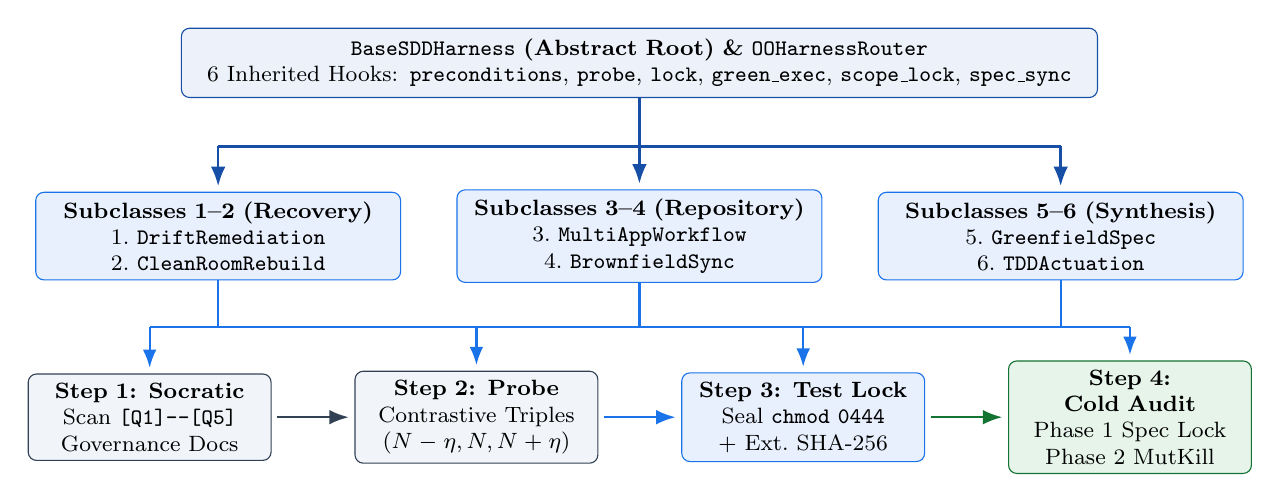
\begin{tikzpicture}[x=1cm,y=1cm,>=Latex]
  % Tier 1 (Top Root): Abstract Base Class + Router (y = 5.20, height = 0.88cm -> bottom at 4.76)
  \node[draw=gNavy, fill=gNavyBg, rounded corners=3pt, text width=11.4cm, minimum height=0.88cm, align=center, font=\footnotesize] (root) at (7.80,5.20)
    {\textbf{\texttt{BaseSDDHarness} (Abstract Root) \& \texttt{OOHarnessRouter}}\\6 Inherited Hooks: \texttt{preconditions}, \texttt{probe}, \texttt{lock}, \texttt{green\_exec}, \texttt{scope\_lock}, \texttt{spec\_sync}};

  % Tier 2 (Middle): 3 Branching Domain Subclass Pairs (y = 3.00, height = 1.05cm -> exactly 3 lines each!)
  \node[draw=gBlue, fill=gBlueBg, rounded corners=3pt, text width=4.4cm, minimum height=1.05cm, align=center, font=\footnotesize] (sub1) at (2.45,3.00)
    {\textbf{Subclasses 1--2 (Recovery)}\\1.\ \texttt{DriftRemediation}\\2.\ \texttt{CleanRoomRebuild}};

  \node[draw=gBlue, fill=gBlueBg, rounded corners=3pt, text width=4.4cm, minimum height=1.05cm, align=center, font=\footnotesize] (sub2) at (7.80,3.00)
    {\textbf{Subclasses 3--4 (Repository)}\\3.\ \texttt{MultiAppWorkflow}\\4.\ \texttt{BrownfieldSync}};

  \node[draw=gBlue, fill=gBlueBg, rounded corners=3pt, text width=4.4cm, minimum height=1.05cm, align=center, font=\footnotesize] (sub3) at (13.15,3.00)
    {\textbf{Subclasses 5--6 (Synthesis)}\\5.\ \texttt{GreenfieldSpec}\\6.\ \texttt{TDDActuation}};

  % Orthogonal Inheritance Tree Bus (Tier 1 -> Tier 2: 1.23cm vertical gap, bus at y=4.14)
  \draw[line width=0.9pt, draw=gNavy] (root.south) -- (7.80,4.14);
  \draw[line width=0.9pt, draw=gNavy] (2.45,4.14) -- (13.15,4.14);
  \draw[->, line width=0.9pt, draw=gNavy, shorten >=2pt] (2.45,4.14) -- (sub1.north);
  \draw[->, line width=0.9pt, draw=gNavy, shorten >=2pt] (7.80,4.14) -- (sub2.north);
  \draw[->, line width=0.9pt, draw=gNavy, shorten >=2pt] (13.15,4.14) -- (sub3.north);

  % Tier 3 (Bottom): 4-Step Sequential Inner Execution Pipeline (y = 0.70, text width = 2.85cm -> outer width ~3.10cm, 1.05cm gaps!)
  \node[draw=gSlate, fill=gSlateBg, rounded corners=3pt, text width=2.85cm, minimum height=1.05cm, align=center, font=\footnotesize] (st1) at (1.58,0.70)
    {\textbf{Step 1: Socratic}\\Scan \texttt{[Q1]--[Q5]}\\Governance Docs};

  \node[draw=gSlate, fill=gSlateBg, rounded corners=3pt, text width=2.85cm, minimum height=1.05cm, align=center, font=\footnotesize] (st2) at (5.73,0.70)
    {\textbf{Step 2: Probe}\\Contrastive Triples\\$(N-\eta, N, N+\eta)$};

  \node[draw=gBlue, fill=gBlueBg, rounded corners=3pt, text width=2.85cm, minimum height=1.05cm, align=center, font=\footnotesize] (st3) at (9.88,0.70)
    {\textbf{Step 3: Test Lock}\\Seal \texttt{chmod 0444}\\+ Ext.\ SHA-256};

  \node[draw=evalPass, fill=evalPassBg, rounded corners=3pt, text width=2.85cm, minimum height=1.05cm, align=center, font=\footnotesize] (st4) at (14.03,0.70)
    {\textbf{Step 4: Cold Audit}\\Phase 1 Spec Lock\\Phase 2 MutKill};

  % Clean Orthogonal Bus from Subclasses (Tier 2) to Execution Pipeline (Tier 3: 1.25cm vertical gap, bus at y=1.85)
  \draw[line width=0.8pt, draw=gBlue] (sub1.south) -- (2.45,1.85);
  \draw[line width=0.8pt, draw=gBlue] (sub2.south) -- (7.80,1.85);
  \draw[line width=0.8pt, draw=gBlue] (sub3.south) -- (13.15,1.85);
  \draw[line width=0.8pt, draw=gBlue] (1.58,1.85) -- (14.03,1.85);
  \draw[->, line width=0.8pt, draw=gBlue, shorten >=2pt] (1.58,1.85) -- (st1.north);
  \draw[->, line width=0.8pt, draw=gBlue, shorten >=2pt] (5.73,1.85) -- (st2.north);
  \draw[->, line width=0.8pt, draw=gBlue, shorten >=2pt] (9.88,1.85) -- (st3.north);
  \draw[->, line width=0.8pt, draw=gBlue, shorten >=2pt] (14.03,1.85) -- (st4.north);
  \draw[->, line width=0.9pt, draw=gSlate, shorten >=2pt, shorten <=2pt] (st1.east) -- (st2.west);
  \draw[->, line width=0.9pt, draw=gBlue, shorten >=2pt, shorten <=2pt] (st2.east) -- (st3.west);
  \draw[->, line width=0.9pt, draw=evalPass, shorten >=2pt, shorten <=2pt] (st3.east) -- (st4.west);
\end{tikzpicture}
\caption{Object-oriented class hierarchy and four-stage execution pipeline of the Contract-Locked Dual-Stage Inner Execution Harness (Arm D). \texttt{BaseSDDHarness} defines six verification hooks inherited across six frozen domain subclasses dispatched by \texttt{OOHarnessRouter} (top and middle tiers), which parameterize the four-stage execution pipeline (bottom tier): Socratic contract elicitation, $(N-\eta, N, N+\eta)$ boundary probing, physical \texttt{chmod 0444} + external SHA-256 test locking, and fresh-context Two-Stage Cold Auditing ($\mathcal{P}_{\text{AST}}$).}
\label{fig:ooharness_uml}
\end{figure}

\begin{enumerate}[leftmargin=1.5em,itemsep=3pt,topsep=3pt]
  \item \textbf{Step 1: Socratic Contract-Consistency Elicitation and Object-Oriented Subclass Routing (\texttt{OOHarnessRouter}).} Extending \texttt{ClarifyGPT} \cite{mu2024clarifygpt}, \texttt{AutoHarness} \cite{lou2026autoharness}, and \texttt{OO-Harness} \cite{li2026ooharness}, \texttt{BaseSDDHarness} defines six inherited governance hooks that execute unconditionally across all six subclasses:
  \begin{itemize}[leftmargin=1.5em,itemsep=1pt,topsep=1pt]
    \item \texttt{check\_preconditions}: Executes requirement ID traceability and a domain-agnostic Socratic contract-consistency scan over the prompt and any auxiliary repository \texttt{*.md} governance files discovered via recursive \texttt{glob("**/*.md", recursive=True)} (such as \texttt{DOMAIN\_GOVERNANCE.md} or \texttt{openspec/specs/SPEC.md}, which are authored as natural-language prose policy documents without \texttt{[Q1]}--\texttt{[Q5]} tags). Whenever the prompt faces a design choice with multiple plausible options, this pre-coding check inspects five universal state-machine invariants ([Q1] rounding/remainder tie-breaking, [Q2] interval endpoint inclusivity, [Q3] multi-bucket deduction priority, [Q4] state-transition precedence under competing triggers, and [Q5] idempotency/error handling) together with an open-ended catch-all clause [Q*] covering concurrency, encoding, or schema evolution; in autonomous benchmark runs, [Q1]--[Q5] and [Q*] are resolved against discovered repository \texttt{*.md} governance files (with interactive developer prompting \cite{mu2024clarifygpt} disabled during blind benchmark evaluation).
    \item \texttt{probe\_boundaries}: Synthesizes contrastive boundary tests across extracted numerical and categorical thresholds.
    \item \texttt{lock\_red\_tests}: Seals red-phase test files via \texttt{chmod 0444} permissions and an external SHA-256 manifest.
    \item \texttt{verify\_green\_execution}: Verifies full test suite pass execution.
    \item \texttt{audit\_out\_of\_scope\_locks}: Enforces scope locks by rejecting unrequested \texttt{\# TODO} stub implementations.
    \item \texttt{verify\_spec\_sync}: Synchronizes inter-loop milestone deltas with the living SSOT specification.
  \end{itemize}
  \texttt{OOHarnessRouter} inspects workspace filesystem state and prompt headers using a deterministic Python six-way \texttt{if/elif/else} cascade evaluated in the exact order below to specialize domain prompt directives while retaining all six base verification hooks:
  \begin{enumerate}[leftmargin=1.5em,itemsep=1pt,topsep=1pt]
    \item \texttt{CleanRoomRebuildHarness}: Evaluated first at milestone $t > 1$ when clean-room source deletion leaves non-test production \texttt{*.py} count at $0$ while an outer specification file (\texttt{openspec/specs/SPEC.md}, \texttt{specs/}, or \texttt{requirements.md}) exists; adds full \texttt{REQ-XXXX} rebuild traceability.
    \item \texttt{DriftRemediationHarness}: Triggered when pre-existing \texttt{test\_*.py} files exist and fail \texttt{unittest} (such as \texttt{pass}-stubbed \texttt{Commit0} modules where non-test \texttt{*.py} count $\ge 1$), or when \texttt{audit\_outer\_spec\_hygiene} (\texttt{compute\_contradiction\_density}) returns \texttt{spec\_contradictions > 0}; overrides \texttt{lock\_red\_tests} to immediately seal pre-existing \texttt{test\_*.py} before any builder turn.
    \item \texttt{MultiAppWorkflowHarness}: Triggered when non-test \texttt{*.py} count is $0$ and prompt/spec text matches \texttt{r"(?i)\textbackslash b(dag|\allowbreak topolog\textbackslash w*|\allowbreak wave|\allowbreak upstream)\textbackslash b"}; emphasizes precedence-inversion probes.
    \item \texttt{BrownfieldSyncHarness}: Triggered when non-test starter \texttt{*.py} count $\ge 1$ in a multi-module git-tracked brownfield repository with passing baseline regression tests; emphasizes untouched legacy method preservation.
    \item \texttt{GreenfieldSpecHarness}: Triggered when non-test \texttt{*.py} count is $0$ and the prompt matches \texttt{r"(\textbackslash\$\textbackslash\$|\textbackslash begin\textbackslash\{|REQ-\textbackslash d+)"}; dispatches directly to formal boundary extraction.
    \item \texttt{TDDActuationHarness}: Default fallback for standard synthesis tasks (including single-function starter stubs in \texttt{BigCodeBench} and \texttt{EvalPlus}).
  \end{enumerate}
  All six subclass definitions were authored prior to benchmark task design and held strictly frozen across all 252 benchmark trials (across the 252 trials, \texttt{BrownfieldSyncHarness} activated on all 60 \texttt{SWE-bench Verified} trials, \texttt{DriftRemediationHarness} activated on the 60 \texttt{Commit0} trials with failing stubbed starter suites, \texttt{TDDActuationHarness} activated on the 120 \texttt{BigCodeBench} and \texttt{EvalPlus} trials, and \texttt{CleanRoomRebuildHarness} activated on the 12 \texttt{Commit0-Evo} Milestone 5 clean-room rebuilds).
  \item \textbf{Step 2: Contrastive Boundary Probing (\texttt{Harness\textsuperscript{2}} \texttt{Propose-Probe-Compose}).} Following \texttt{Harness\textsuperscript{2}} \cite{xu2026harness2}, before writing production code, \texttt{probe\_boundaries} scans the active specification files passed from Step 1 (the task specification prompt in \texttt{Arm C}, plus any repository governance or specification files such as \texttt{openspec/specs/SPEC.md} discovered by Step 1 in \texttt{Arm D}) with a deterministic regex constant and unit-normalization extractor (filtering out requirement identifiers \texttt{REQ-\textbackslash d+}, ISO dates \texttt{\textbackslash d\{4\}-\textbackslash d\{2\}-\textbackslash d\{2\}}, and section headers, scaling multiplier suffixes such as \texttt{500k} $\to 500000$ while stripping unit-only suffixes such as \texttt{50 bps} $\to 50$ and \texttt{60s} $\to 60$ into canonical integer domain units, identifying integer literals $N$ with step $\eta = 1$, decimal/float literals with step $\eta = 10^{-d}$ at precision $d$, comparison operators \texttt{<}, \texttt{<=}, \texttt{>}, \texttt{>=}, and uppercase categorical status literals, while parsing starter \texttt{*.py} ASTs in brownfield tasks solely for public class/method signatures and ignoring potentially buggy starter constants). In plain terms, boundary probing automatically tests one step below, right on, and one step above every threshold $N$ so off-by-one \texttt{<} vs.\ \texttt{<=} bugs cannot hide. Specifically, it pairs these extracted constants with an LLM test-synthesis prompt constrained to emit unit test assertions inside a single \texttt{unittest.TestCase} subclass at every extracted boundary triple $(N - \eta, N, N + \eta)$ and $(-\eta, 0, \eta)$ while holding orthogonal parameters at deterministic valid interior values (using $\lfloor(a+b)/2\rfloor$ for integer intervals $[a, b]$, exact \texttt{decimal.Decimal} midpoint $\text{round}((a+b)/2, d)$ for decimal bounds, and $N_0 \pm 10\eta$ for lower- or upper-bounded intervals while preserving coupled parameter ordering such as \texttt{min\_val <= max\_val}), plus pairwise precedence-inversion tests where competing categorical states (e.g., upstream \texttt{BLOCKED} vs.\ local \texttt{FAILED}) hold simultaneously on the same entity.
  \item \textbf{Step 3: Physical Read-Only Test Lock (\texttt{chmod 0444} and Out-of-Workspace SHA-256 Manifest).} Once the red-phase unit test file \texttt{test\_*.py} is authored in Step 2 (or immediately upon workspace initialization when \texttt{DriftRemediationHarness} detects a pre-existing red-phase test suite), \texttt{lock\_red\_tests} sets POSIX file permissions to \texttt{0444} (read-only) and records its SHA-256 digest both in \texttt{.readonly\_test\_lock.sha256} and in external orchestrator memory outside the agent's writable directory. If an agent attempts to weaken a failing test via \texttt{chmod +w}, Phase 1 of the Cold Audit detects the hash mismatch against the external orchestrator's SHA-256 digest and rejects the build.
  \item \textbf{Step 4: Two-Stage Cold Audit and Constructive AST Prefix Unlock-and-Reseal Protocol ($\mathcal{P}_{\text{AST}}$).} After the test suite passes, each audit submission executes a 0-token deterministic Python pre-check (\texttt{ast} and \texttt{hashlib} lock verification) followed by a single fresh-context Cold Auditor subagent turn invoked with zero builder chat history \cite{rensin2026elephant,kenton2026debate,sahoo2025double} that evaluates two sequential phases:
  \begin{itemize}[leftmargin=1.5em,itemsep=1pt,topsep=1pt]
    \item \textbf{Phase 1 (Spec Compliance \& Anti-Tamper Gate):} Audits the implementation for unstated assumptions that affect required domain behavior, rejects mock-only subterfuge such as \texttt{unittest.mock.MagicMock} replacing core domain methods, verifies non-implementation of out-of-scope \texttt{\# TODO} stubs, and confirms the external SHA-256 test lock (in all 60 \texttt{Arm D} inner-loop trials, the Stage 1 Builder leaves the \texttt{chmod 0444}-locked starter test file untouched, verified via \texttt{git checkout} and \texttt{check\_test\_tamper}, and authors a dedicated contract test suite in \texttt{tests/\allowbreak test\_unit\_contract.py}, which the Stage 2 Cold Independent Auditor executes alongside the starter suite before issuing its JSON \texttt{APPROVE}/\texttt{REJECT} gate verdict).
    \item \textbf{Phase 2 (Static AST \& Branch Boundary Audit):} Audits boundary mutation adequacy via static AST and branch inspection across \emph{all} public methods of the target module, with zero visibility into the sealed evaluation mutants in \texttt{grade\_all\_runs.py}.
  \end{itemize}
  When a workspace locks all test assertions inside a single read-only \texttt{test\_*.py} file and Phase 2 identifies an unprobed method or boundary, the Cold Auditor can emit missing \texttt{test\_zz\_audit\_r\{r\}\_\{idx\}\_*} methods in that same response so the external orchestrator mediates a 0-LLM-turn \textbf{monitored append-only AST unlock-and-reseal pass} enforcing a strict \emph{constructive AST prefix invariant} $\mathcal{P}_{\text{AST}}(\mathcal{T}_{\text{pre}}, \mathcal{T}_{\text{post}}) = 1$ (across our 60 \texttt{Arm D} inner-loop trials where Stage 1 authored \texttt{tests/\allowbreak test\_unit\_contract.py}, the Stage 2 Cold Independent Auditor verified both suites and returned \texttt{APPROVE} on all $60/60$ trials without requiring a fallback AST splice). In plain terms, $\mathcal{P}_{\text{AST}}$ enforces an append-only rule on the test file's syntax tree: every existing test stays untouched at the top of the file, and new auditor tests can only be added at the bottom. Formally, the orchestrator parses the locked \texttt{test\_*.py} into an abstract syntax tree $\mathcal{T}_{\text{pre}}$, temporarily toggles \texttt{chmod 0644} to splice the Cold Auditor's synthesized \texttt{test\_zz\_audit\_r\{r\}\_\{idx\}\_*} methods into the end of the target \texttt{TestCase} class body (or into $\text{body}(\text{Module}_{\text{post}}) = \text{body}(\text{Module}_{\text{pre}}) \mathbin{\Vert} [f_1, \dots, f_m]$ for module-level \texttt{pytest} test files), and programmatically checks via Python's \texttt{ast} module (\texttt{verify\_constructive\_ast\_prefix\_splice} in \texttt{grade\_all\_runs.py}) before resealing (\texttt{chmod 0444} and updating the out-of-workspace SHA-256 manifest) that $\mathcal{T}_{\text{post}}$ is identical in \texttt{ast.dump()} to $\mathcal{T}_{\text{pre}}$ everywhere outside the target container body (keeping top-level imports frozen while permitting function-scoped inline \texttt{import} statements restricted to pure standard-library modules) and that $\text{body}(\text{ClassDef}_{\text{post}}) = \text{body}(\text{ClassDef}_{\text{pre}}) \mathbin{\Vert} [f_1, \dots, f_m]$. Each appended node $f_i$ must be an \texttt{ast.FunctionDef} whose round-indexed name \texttt{test\_zz\_audit\_r\{r\}\_\{idx\}\_*} compares lexicographically greater than every pre-existing \texttt{test\_*} method name in $\text{ClassDef}_{\text{pre}}$ ($f_i.\text{name} > m_{\text{pre}}$ for all $m_{\text{pre}} \in \text{ClassDef}_{\text{pre}}$, dynamically scaling the \texttt{z}-prefix above $\max(m_{\text{pre}})$ so \texttt{unittest.TestLoader}'s alphabetical sort executes all pre-existing locked tests strictly before any appended audit test across rounds $r \in \{1, 2, 3\}$), is disjoint from all existing method and attribute names in $\text{ClassDef}_{\text{pre}}$ (preventing duplicate method shadowing or \texttt{setUp}/\texttt{tearDown}/\texttt{setUpClass} overrides), has an empty \texttt{decorator\_list}, and contains no \texttt{global}/\texttt{nonlocal} statements or AST attribute/subscript writes, deletions, or mutating calls (\texttt{ast.Store()}/\texttt{ast.Del()} on \texttt{self.*} or outer-scope attributes, \texttt{setattr}, \texttt{delattr}, \texttt{mock.patch}, \texttt{eval}, \texttt{exec}, \texttt{\_\_import\_\_}, \texttt{open(..., "w"|"a")}, \texttt{os.chmod}, or fixture \texttt{.clear()}/\texttt{.pop()}) targeting \texttt{self.\_\_class\_\_}, \texttt{sys.modules}, \texttt{builtins}, or imported production module symbols. The resealed test suite is then re-executed under a bounded retry ceiling $K_{\max} = 3$; if any newly appended test fails against the current implementation, control returns to Step 3 under the updated read-only lock to repair the production code.
  \item \textbf{Inter-Loop Handoff Gate and Dual Specification Synchronization (\texttt{verify\_spec\_sync}).} In multi-milestone workflows, inner-loop Step 4 Cold Audit sign-off is a mandatory programmatic precondition for outer-loop state transition. Only after Phase 1 and Phase 2 return \texttt{PASS} does \texttt{verify\_spec\_sync} run \texttt{compute\_contradiction\_density} over the candidate specification state to enforce Preconditions (a)--(c) (identifying overlapping variable footprints even when prompts omit explicit \texttt{REQ-XXXX} IDs), invoke the forward compiler $\Phi(S_{t-1}, \Delta_t)$ on forward milestones (or dispatch to $\Phi_{\text{seq}}^{-1}$ on historical rollback milestones) to update the living capability specification \texttt{openspec/specs/\allowbreak SPEC.md} (instantiated on \texttt{TinyDB} in \texttt{Commit0-Evo}), append the post-rename pre-image record $A_t$ to the historical delta archive \texttt{conductor/tracks/\allowbreak delta\_history.md}, and verify exact round-trip invertibility $S_{t-1} = \Phi^{-1}(S_t, \Delta_t, \text{pre}(S'_{t-1}, \Delta_t))$ and bidirectional \texttt{REQ-XXXX} threshold parity.
\end{enumerate}

\begin{figure}[t!]
\centering
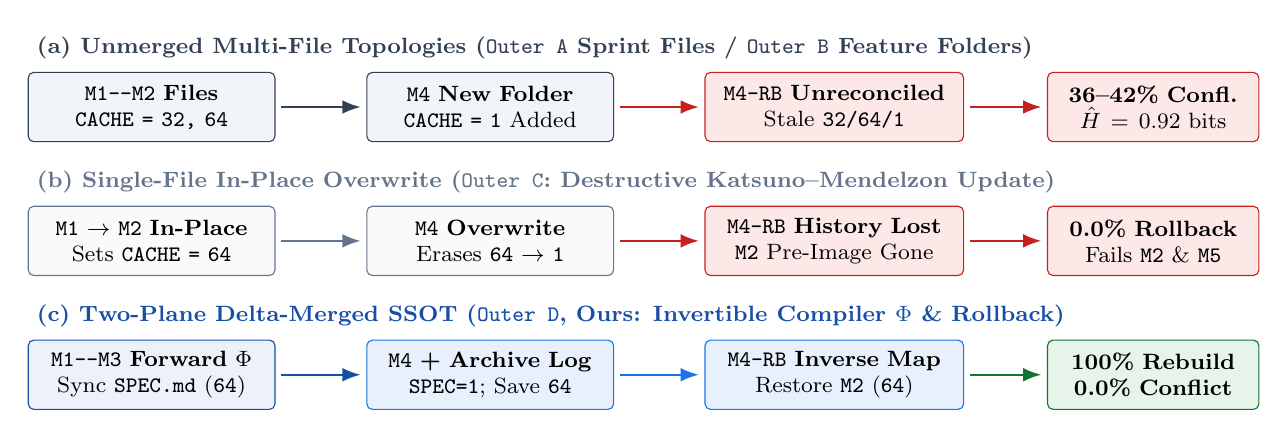
\begin{tikzpicture}[x=1cm,y=1cm,>=Latex]
  % Row (a): Outer A / Outer B (Unmerged Multi-File / Feature Folders) -> y = 4.10
  \node[anchor=west, font=\footnotesize, text=gSlate] at (0.0,4.85)
    {\textbf{(a) Unmerged Multi-File Topologies (\texttt{Outer A} Sprint Files / \texttt{Outer B} Feature Folders)}};
  \node[draw=gSlate, fill=gSlateBg, rounded corners=2pt, text width=2.90cm, minimum height=0.88cm, align=center, font=\footnotesize] (a1) at (1.58,4.10)
    {\textbf{\texttt{M1--M2} Files}\\\texttt{CACHE = 32, 64}};
  \node[draw=gSlate, fill=gSlateBg, rounded corners=2pt, text width=2.90cm, minimum height=0.88cm, align=center, font=\footnotesize] (a2) at (5.88,4.10)
    {\textbf{\texttt{M4} New Folder}\\\texttt{CACHE = 1} Added};
  \node[draw=evalFail, fill=evalFailBg, rounded corners=2pt, text width=3.05cm, minimum height=0.88cm, align=center, font=\footnotesize] (a3) at (10.25,4.10)
    {\textbf{\texttt{M4-RB} Unreconciled}\\Stale \texttt{32/64/1}};
  \node[draw=evalFail, fill=evalFailBg, rounded corners=2pt, text width=2.45cm, minimum height=0.88cm, align=center, font=\footnotesize] (a4) at (14.30,4.10)
    {\textbf{36--42\% Confl.}\\$\hat{H}=0.92$ bits};
  \draw[->, line width=0.8pt, draw=gSlate, shorten >=2pt, shorten <=2pt] (a1.east) -- (a2.west);
  \draw[->, line width=0.8pt, draw=evalFail, shorten >=2pt, shorten <=2pt] (a2.east) -- (a3.west);
  \draw[->, line width=0.8pt, draw=evalFail, shorten >=2pt, shorten <=2pt] (a3.east) -- (a4.west);

  % Row (b): Outer C (Single-File In-Place EARS Overwriting) -> y = 2.40
  \node[anchor=west, font=\footnotesize, text=gGray] at (0.0,3.15)
    {\textbf{(b) Single-File In-Place Overwrite (\texttt{Outer C}: Destructive Katsuno--Mendelzon Update)}};
  \node[draw=gGray, fill=gGrayBg, rounded corners=2pt, text width=2.90cm, minimum height=0.88cm, align=center, font=\footnotesize] (b1) at (1.58,2.40)
    {\textbf{\texttt{M1} $\to$ \texttt{M2} In-Place}\\Sets \texttt{CACHE = 64}};
  \node[draw=gGray, fill=gGrayBg, rounded corners=2pt, text width=2.90cm, minimum height=0.88cm, align=center, font=\footnotesize] (b2) at (5.88,2.40)
    {\textbf{\texttt{M4} Overwrite}\\Erases \texttt{64} $\to$ \texttt{1}};
  \node[draw=evalFail, fill=evalFailBg, rounded corners=2pt, text width=3.05cm, minimum height=0.88cm, align=center, font=\footnotesize] (b3) at (10.25,2.40)
    {\textbf{\texttt{M4-RB} History Lost}\\\texttt{M2} Pre-Image Gone};
  \node[draw=evalFail, fill=evalFailBg, rounded corners=2pt, text width=2.45cm, minimum height=0.88cm, align=center, font=\footnotesize] (b4) at (14.30,2.40)
    {\textbf{0.0\% Rollback}\\Fails \texttt{M2} \& \texttt{M5}};
  \draw[->, line width=0.8pt, draw=gGray, shorten >=2pt, shorten <=2pt] (b1.east) -- (b2.west);
  \draw[->, line width=0.8pt, draw=evalFail, shorten >=2pt, shorten <=2pt] (b2.east) -- (b3.west);
  \draw[->, line width=0.8pt, draw=evalFail, shorten >=2pt, shorten <=2pt] (b3.east) -- (b4.west);

  % Row (c): Outer D (Two-Plane Delta-Merged SSOT, Ours) -> y = 0.70
  \node[anchor=west, font=\footnotesize, text=gNavy] at (0.0,1.45)
    {\textbf{(c) Two-Plane Delta-Merged SSOT (\texttt{Outer D}, Ours: Invertible Compiler $\Phi$ \& Rollback)}};
  \node[draw=gNavy, fill=gNavyBg, rounded corners=2pt, text width=2.90cm, minimum height=0.88cm, align=center, font=\footnotesize] (c1) at (1.58,0.70)
    {\textbf{\texttt{M1--M3} Forward $\Phi$}\\Sync \texttt{SPEC.md} (\texttt{64})};
  \node[draw=gBlue, fill=gBlueBg, rounded corners=2pt, text width=2.90cm, minimum height=0.88cm, align=center, font=\footnotesize] (c2) at (5.88,0.70)
    {\textbf{\texttt{M4} + Archive Log}\\\texttt{SPEC=1}; Save \texttt{64}};
  \node[draw=gBlue, fill=gBlueBg, rounded corners=2pt, text width=3.05cm, minimum height=0.88cm, align=center, font=\footnotesize] (c3) at (10.25,0.70)
    {\textbf{\texttt{M4-RB} Inverse Map}\\Restore \texttt{M2} (\texttt{64})};
  \node[draw=evalPass, fill=evalPassBg, rounded corners=2pt, text width=2.45cm, minimum height=0.88cm, align=center, font=\footnotesize] (c4) at (14.30,0.70)
    {\textbf{100\% Rebuild}\\\textbf{0.0\% Conflict}};
  \draw[->, line width=0.8pt, draw=gNavy, shorten >=2pt, shorten <=2pt] (c1.east) -- (c2.west);
  \draw[->, line width=0.8pt, draw=gBlue, shorten >=2pt, shorten <=2pt] (c2.east) -- (c3.west);
  \draw[->, line width=0.8pt, draw=evalPass, shorten >=2pt, shorten <=2pt] (c3.east) -- (c4.west);
\end{tikzpicture}
\caption{Comparison of longitudinal specification state evolution across Milestones \texttt{M1}--\texttt{M5} on \texttt{Commit0-Evo} (\texttt{TinyDB}). \textbf{(a)} Unmerged multi-file topologies (\texttt{Outer A} and \texttt{Outer B}) leave superseded constants active across files ($36.4\%$--$41.7\%$ contradiction density, degrading \texttt{Outer B} to $66.7\%$ and $\hat{H}=0.92\text{ bits}$). \textbf{(b)} Single-file in-place overwriting (\texttt{Outer C}) eliminates active contradictions but erases the Milestone 2 pre-image at \texttt{M4}, collapsing to $0.0\%$ on \texttt{M4-RB} rollback. \textbf{(c)} Our Two-Plane SSOT (\texttt{Outer D}) pairs forward compilation $\Phi$ in \texttt{openspec/specs/SPEC.md} with pre-image archiving in \texttt{conductor/tracks/delta\_history.md} and supports exact inverse rollback $\Phi_{\text{seq}}^{-1}$ ($100.0\%$ rebuild and rollback parity with $0.0\%$ conflicts).}
\label{fig:two_plane_timeline}
\end{figure}

\section{Concrete Code and Specification Diff Case Studies}
\label{sec:case_studies}

Before presenting aggregate metrics across all 252 multi-subagent trials, we examine three concrete trajectory case studies from our benchmark runs that illustrate how inner-loop test tampering, brownfield domain defects, and outer-loop specification drift arise in real subagent executions.

\subsection{Case Study 1 on Destructive Starter-Test Overwriting and Baseline Test Tampering}
\label{subsec:case_study_inner}

A central empirical finding of our 240-trial inner-loop evaluation is that instructing an autonomous coding agent to follow a strict test-driven development loop (\texttt{Arm B: Procedural TDD}) or an object-oriented verification checklist (\texttt{Arm C: OO-Harness}) without physical read-only test locks substantially increases baseline test tampering relative to unconstrained vibe coding (\texttt{Arm A}) \cite{denison2024sycophancy,zhong2025impossiblebench}: across all 240 trials, baseline test tampering rises from $5.0 \pm 0.0\%$ ($3/60$) in \texttt{Arm A} to $18.3 \pm 2.9\%$ ($11/60$) in \texttt{Arm B} and $23.3 \pm 2.9\%$ ($14/60$) in \texttt{Arm C}, before dropping to $0.0 \pm 0.0\%$ ($0/60$) under our Contract-Locked Dual-Stage Harness (\texttt{Arm D}).

Inspecting the AST tamper audit logs across all 28 tampered trials reveals two distinct mechanisms: in $27/28$ tampered trials, the subagent triggered \texttt{baseline\_\allowbreak test\_func\_\allowbreak removed} by overwriting the starter test file from scratch when authoring its TDD test suite, and in $1/28$ trials (\texttt{humaneval\_\_129} Run 2 in \texttt{Arm C}), the subagent triggered \texttt{baseline\_\allowbreak assertion\_\allowbreak altered} by editing a baseline docstring example assertion in place. Specifically, on \texttt{BigCodeBench/10} (\texttt{bigcodebench\_\_10}), \texttt{BigCodeBench/22} (\texttt{bigcodebench\_\_22}), \texttt{BigCodeBench/24} (\texttt{bigcodebench\_\_24}), and \texttt{BigCodeBench/27} (\texttt{bigcodebench\_\_27}), the workspace initializes \texttt{tests/\allowbreak test\_solution.py} with a \texttt{TestBaselineContract} suite containing baseline smoke assertions (such as \texttt{test\_baseline\_\allowbreak tuple\_stats} checking 3-tuple \texttt{(mean, median, mode)} statistics on \texttt{task\_func(T1, RANGE=100)}). When \texttt{Arm B} (in Run 2 on \texttt{bigcodebench\_\_10}, Run 1 on \texttt{bigcodebench\_\_22}, and Runs 2 and 3 on \texttt{bigcodebench\_\_24}) and \texttt{Arm C} (in all 3 runs on \texttt{bigcodebench\_\_10} and Run 3 on \texttt{bigcodebench\_\_27}) executed their red-phase test generation step over a writable \texttt{tests/} directory, the subagents replaced the entire \texttt{tests/\allowbreak test\_solution.py} file with a newly authored \texttt{TestTaskFunc} class, deleting \texttt{test\_baseline\_\allowbreak tuple\_stats}:
\begin{verbatim}
# Tampered starter test in tests/test_solution.py (bigcodebench__10)
- class TestBaselineContract(unittest.TestCase):
-     def test_baseline_tuple_stats(self): ...
+ class TestTaskFunc(unittest.TestCase):  # Deleted baseline_test_func
\end{verbatim}
The same destructive test-replacement behavior occurs on \texttt{Commit0} from-scratch library synthesis (\texttt{commit0\_\_\allowbreak tinydb\_\allowbreak middlewares}, \texttt{storages}, \texttt{operations}, \texttt{queries}, and \texttt{wcwidth\_core}), where \texttt{Arm B} tampered with baseline tests in $46.7 \pm 23.1\%$ ($7/15$) of trials and \texttt{Arm C} tampered in $53.3 \pm 11.5\%$ ($8/15$) of trials by deleting failing starter test functions (\texttt{baseline\_\allowbreak test\_func\_\allowbreak removed}) or replacing \texttt{JSONStorage} handle and \texttt{CachingMiddleware} flush tests in \texttt{tests/\allowbreak test\_middlewares.py} and \texttt{tests/\allowbreak test\_storages.py}. In \texttt{Arm D}, \texttt{chmod 0444} permissions paired with external SHA-256 manifest verification and Stage 2 Cold Independent Auditing blocked every test-tampering attempt across all 60 \texttt{Arm D} trials ($0.0 \pm 0.0\%$ tamper rate), forcing the builder subagent to keep all pre-existing starter test functions intact while constructively appending new \texttt{test\_*} functions.

\subsection{Case Study 2 on Brownfield Symbolic Algebra Bugs in \texttt{SWE-bench Verified}}
\label{subsec:case_study_swebench}

On \texttt{SWE-bench Verified} (\texttt{SymPy 1.12}), all four harnesses maintained $0.0 \pm 0.0\%$ test tampering because the repository test files are large, established regression suites, yet raw oracle pass rates separated \texttt{Arm A} ($93.3 \pm 11.5\%$, $14/15$) and \texttt{Arm B} ($86.7 \pm 11.5\%$, $13/15$) from \texttt{Arm C} ($100.0 \pm 0.0\%$, $15/15$) and \texttt{Arm D} ($100.0 \pm 0.0\%$, $15/15$). In \texttt{sympy\_\_sympy-23950}, \texttt{Contains(x, Reals).as\_set()} erroneously returned \texttt{Contains(x, Reals)} (not a \texttt{Set}) instead of \texttt{Reals}, causing \texttt{Piecewise((1, Contains(x, Reals)), (0, True))} to raise an \texttt{AttributeError} during interval evaluation. In Run 3, both \texttt{Arm A} and \texttt{Arm B} patched \texttt{Contains.as\_set()} in \texttt{sympy/sets/\allowbreak contains.py} by returning \texttt{self.args[1]} only under a restrictive type check that failed composite set expressions, yet self-reported $100.0\%$ task completion because their narrow reproduction test checked only a single scalar symbol. Similarly, in Run 1 on \texttt{sympy\_\_sympy-24443} (\texttt{sympy/\allowbreak combinatorics/\allowbreak homomorphisms.py}), \texttt{Arm B} mishandled inverted permutation generators in \texttt{\_check\_\allowbreak homomorphism} when checking relators of a \texttt{PermutationGroup}, failing the held-out oracle. In \texttt{Arm D}, contrastive boundary probing across symbolic group generators and Stage 2 Cold Auditing verified both \texttt{Contains.as\_set()} return invariants and relator image products, achieving $100.0 \pm 0.0\%$ ($15/15$) across all three runs and lifting patched-function AST mutation kill rate on \texttt{SWE-bench Verified} from $13.3 \pm 11.5\%$ (\texttt{Arm C}) and $20.0 \pm 0.0\%$ (\texttt{Arm B}) to $37.8 \pm 3.8\%$ (\texttt{Arm D}).

\subsection{Case Study 3 on Longitudinal Specification Contradiction and Rollback in \texttt{Commit0-Evo}}
\label{subsec:case_study_outer}

In our 12-trial outer-loop \texttt{Commit0-Evo} benchmark on \texttt{TinyDB} (\texttt{3 runs} $\times$ \texttt{4 outer topologies} evaluated across 5 sequential capability milestones \texttt{M1}--\texttt{M5}, totaling 60 milestone oracle evaluations), the repository specification evolves across five sprints:
\begin{verbatim}
M1 (Table & Clamp)     -> count_all(); clamp(swap); WRITE_CACHE_SIZE = 32
M2 (Cache Batching)    -> WRITE_CACHE_SIZE = 64; add pending_writes
M3 (Query Validation)  -> clamp raises ValueError; add Query.iequals(rhs)
M4 (Strict Lock Mode)  -> WRITE_CACHE_SIZE = 1; delete raises PermissionError
M4-RB & M5 (Rebuild)   -> Rollback M4 to M2/M3 (64) + add read_hits rebuild
\end{verbatim}
Because Milestone 5 includes a mandatory point-in-time historical rollback (\texttt{M4-RB}) that annuls the Milestone 4 Strict Cache Lock (\texttt{WRITE\_CACHE\_SIZE = 1} and \texttt{PermissionError} on \texttt{delete}) back to the Milestone 2/3 caching and validation contracts (\texttt{WRITE\_CACHE\_SIZE = 64}, normal \texttt{delete}, and \texttt{clamp} raising \texttt{ValueError}) alongside clean-room synthesis of \texttt{read\_hits} (\texttt{M5}), the post-trajectory repository state must satisfy \texttt{WRITE\_CACHE\_SIZE == 64} alongside all active \texttt{M1}--\texttt{M5} contracts. Under \texttt{Outer B} (Feature-Isolated Spec Directories \texttt{specs/\allowbreak feat\_*/\allowbreak spec.md}), each capability domain is stored in one of 5 unnumbered feature folders (\texttt{feat\_\allowbreak table\_\allowbreak and\_\allowbreak clamp}, \texttt{feat\_\allowbreak caching\_\allowbreak middleware}, \texttt{feat\_\allowbreak queries\_\allowbreak and\_\allowbreak validation}, \texttt{feat\_\allowbreak strict\_\allowbreak cache\_\allowbreak lock}, and \texttt{feat\_\allowbreak read\_\allowbreak telemetry}) without chronological timestamps. Because superseded clauses remain unmerged across folders, \texttt{feat\_\allowbreak table\_\allowbreak and\_\allowbreak clamp/\allowbreak spec.md} retains \texttt{WRITE\_CACHE\_SIZE = 32}, \texttt{feat\_\allowbreak caching\_\allowbreak middleware/\allowbreak spec.md} states \texttt{WRITE\_CACHE\_SIZE = 64}, and \texttt{feat\_\allowbreak strict\_\allowbreak cache\_\allowbreak lock/\allowbreak spec.md} states \texttt{WRITE\_CACHE\_SIZE = 1}, creating $4.0/11.0$ ($36.4\%$) active contradictory clauses across the 11 requirement clauses in the specification directory. In Run 3 of \texttt{Outer B}, after \texttt{feat\_\allowbreak read\_\allowbreak telemetry/\allowbreak spec.md} annulled the \texttt{M4} lock, the clean-room synthesis subagent encountered the unresolved conflict between \texttt{WRITE\_CACHE\_SIZE = 32} (in \texttt{feat\_\allowbreak table\_\allowbreak and\_\allowbreak clamp/\allowbreak spec.md}) and \texttt{WRITE\_CACHE\_SIZE = 64} (in \texttt{feat\_\allowbreak caching\_\allowbreak middleware/\allowbreak spec.md}) and implemented \texttt{WRITE\_CACHE\_SIZE = 32}, failing the \texttt{M2 Pivot}, \texttt{M4-RB Roll}, and \texttt{M5 Rebuild} checks ($66.7 \pm 57.7\%$, $\hat{H} = 0.92\text{ bits}$). Conversely, under \texttt{Outer C} (Single-File In-Place EARS \texttt{requirements.md}), Milestone 4 (\texttt{REQ-4}) overwrote \texttt{WRITE\_CACHE\_SIZE = 64} in place with \texttt{WRITE\_CACHE\_SIZE = 1} ($0.0\%$ contradictions across its 6 active clauses), permanently erasing the Milestone 2 constant \texttt{64} from the working tree; therefore, when Milestone 5 (\texttt{REQ-6}) instructed the agent to revert to the pre-lock Sprint 3 specification values without stating \texttt{64}, all 3 runs of \texttt{Outer C} fell back to \texttt{TinyDB}'s legacy base default (\texttt{WRITE\_CACHE\_SIZE = 1000}), failing \texttt{M2 Pivot}, \texttt{M4-RB Roll}, and \texttt{M5 Rebuild} ($0.0 \pm 0.0\%$). Under \texttt{Outer D} (Two-Plane Delta-Merged SSOT), \texttt{openspec/specs/\allowbreak SPEC.md} is updated in place via $\Phi$ while every milestone's pre-image delta is archived in \texttt{conductor/tracks/\allowbreak delta\_history.md} (12 active clauses in \texttt{SPEC.md} with 0 conflicts), achieving $100.0 \pm 0.0\%$ ($3/3$) across all five milestones with $0.0\%$ contradiction density and $\hat{H} = 0.00\text{ bits}$.

\begin{table}[t!]
\centering
\caption{Claim-Evidence Map linking each architectural claim to its empirical validation across our 252 genuine multi-subagent trials (240 inner-loop trials + 12 outer-loop multi-milestone trials evaluated across 60 milestone checks, executed by 312 blind subagent invocations including 60 Stage 2 Cold Independent Auditors) on untouched upstream benchmarks.}
\label{tab:claim_evidence}
\footnotesize
\begin{tabularx}{\textwidth}{L{3.1cm} Y L{2.8cm}}
\toprule
\textbf{Architectural Claim} & \textbf{Validating Empirical Evidence (Mean $\pm$ SD Across 3 Runs)} & \textbf{Supporting Suite} \\
\midrule
\textbf{Claim 1: Eliminating Inner-Loop Baseline Test Tampering} & Without physical test locks, TDD/verification prompts increase baseline test tampering from \texttt{5.0~$\pm$~0.0\%} (\texttt{3/60}, Arm A) to \texttt{18.3~$\pm$~2.9\%} (\texttt{11/60}, Arm B) and \texttt{23.3~$\pm$~2.9\%} (\texttt{14/60}, Arm C). Arm D's \texttt{chmod 0444} lock + Cold Audit reduces test tampering to \texttt{0.0~$\pm$~0.0\%} (\texttt{0/60}) across all 4 suites. & Suites 1--4 (\texttt{240} trials), \cref{tab:suite1_results,tab:suite1b_results,fig:per_suite_pareto,fig:suite1_combined_chart} \\
\addlinespace[3pt]
\textbf{Claim 2: Superior Tamper-Free Strict Pass Rate ($\text{Pass}_{\text{strict}}$)} & Across 240 upstream trials, Arm D achieves \texttt{91.7~$\pm$~2.9\%} (\texttt{55/60}) tamper-free strict pass rate ($\text{Oracle} \land \neg\text{Tamper}$), outperforming Arm C (\texttt{70.0~$\pm$~0.0\%}, \texttt{+21.7 pp}), Arm B (\texttt{68.3~$\pm$~5.8\%}, \texttt{+23.4 pp}), and Arm A (\texttt{83.3~$\pm$~2.9\%}, \texttt{+8.4 pp}), with a \texttt{+53.4 pp} strict pass gain on \texttt{Commit0} (\texttt{86.7\%} vs.\ \texttt{33.3\%}). & \texttt{SWE-bench}, \texttt{Commit0}, \texttt{BigCode}, \texttt{EvalPlus} (\texttt{240} trials), \cref{tab:suite1_results,fig:teaser_chart,fig:per_suite_pareto} \\
\addlinespace[3pt]
\textbf{Claim 3: Patched-Function AST Mutation Adequacy} & Evaluated over Offutt Sufficient-5 AST mutants scoped to modified functions, Arm D achieves the highest overall mutation kill rate (\texttt{70.6~$\pm$~4.6\%}), outperforming Arm A (\texttt{59.6~$\pm$~6.3\%}, \texttt{+11.0 pp}), Arm C (\texttt{61.7~$\pm$~3.8\%}, \texttt{+8.9 pp}), and Arm B (\texttt{66.9~$\pm$~2.1\%}, \texttt{+3.7 pp}). & Suites 1--4 (\texttt{240} trials), \cref{tab:suite1_results,fig:suite1_combined_chart} \\
\addlinespace[3pt]
\textbf{Claim 4: Confirmation Bias \& Per-Task Failure Taxonomy} & Because subagents iterate until local workspace tests pass (\texttt{100.0~$\pm$~0.0\%} self-reported completion), held-out oracle failures induce an \texttt{8.3\%}--\texttt{13.3\%} confirmation bias gap (\texttt{8.3\%} in Arms C \& D on \texttt{commit0\_\_tinydb\_queries} and \texttt{bigcodebench\_\_6}), while Arm D achieves \texttt{100.0~$\pm$~0.0\%} on \texttt{SWE-bench} and \texttt{EvalPlus}. & Per-Task Audit (\texttt{20} upstream tasks), \cref{tab:suite1b_results,subsec:suite1b_results} \\
\addlinespace[3pt]
\textbf{Claim 5: Longitudinal SSOT Rebuildability \& Rollback ($\Phi, \Phi_{\text{seq}}^{-1}$)} & Across 12 multi-milestone \texttt{Commit0-Evo} trials (60 milestone builds on \texttt{TinyDB}), Outer D uniquely achieves \texttt{100.0~$\pm$~0.0\%} on forward evolution (\texttt{M1}--\texttt{M3}), \texttt{M4} $\to$ \texttt{M2} rollback (\texttt{M4-RB}), and \texttt{M5} clean-room rebuild with \texttt{0.0\%} contradiction density and $\hat{H} = 0.00\text{ bits}$. & Suite 5 \texttt{Commit0-Evo} (\texttt{12} trials, \texttt{60} builds), \cref{tab:suite2_results,fig:suite2_rollback_chart,fig:suite3_entropy_chart} \\
\bottomrule
\end{tabularx}
\end{table}

\section{Experimental Setup}
\label{sec:setup}

We evaluate our architecture across five benchmark suites totaling \textbf{252 genuine multi-subagent trials} (240 inner-loop trials across Suites 1--4 and 12 longitudinal \texttt{Commit0-Evo} trials evaluated across 60 milestone checks in Suite 5, executed by \textbf{312 blind subagent invocations} comprising 240 inner-loop Builder subagents, 60 fresh-context Stage 2 Cold Independent Auditor subagents in \texttt{Arm D}, and 12 multi-milestone clean-room synthesis subagents across the \texttt{Commit0-Evo} trajectories; \cref{tab:claim_evidence}). All Builder, Stage 2 Cold Independent Auditor, and Clean-Room Synthesis subagents are instantiated with \texttt{Gemini 3.8 Flash} (\texttt{gemini-3.8-flash}) under default server decoding parameters in fresh, isolated agent sessions with standard POSIX file-editing and test-execution tools (1M-token context window) and zero access to held-out oracle scripts or privileged gold reference files stored in \texttt{privilege\_dir/}. Across the four inner-loop arms, \texttt{Arm A} executes direct single-agent synthesis and test execution without \texttt{BaseSDDHarness} hooks; \texttt{Arm B} executes procedural \texttt{SKILL.md} Red-Green-Refactor TDD prompting without \texttt{OOHarnessRouter}, \texttt{chmod 0444} locks, or cold auditing; \texttt{Arm C} executes \texttt{OOHarnessRouter} subclass dispatch, \texttt{check\_preconditions}, \texttt{probe\_boundaries}, and \texttt{verify\_green\_execution} over a mutable \texttt{tests/} directory without \texttt{chmod 0444} locks or Stage 2 Cold Auditing; and \texttt{Arm D} executes all six \texttt{BaseSDDHarness} hooks (\texttt{check\_preconditions}, \texttt{probe\_boundaries}, \texttt{lock\_red\_tests} with \texttt{chmod 0444} and external SHA-256 verification, \texttt{verify\_green\_execution}, \texttt{audit\_out\_of\_scope\_locks}, and \texttt{verify\_spec\_sync}) paired with the fresh-context Stage 2 Cold Independent Auditor.

\textbf{Suite 1 (\texttt{SWE-bench Verified} Multi-File Brownfield Issue Resolution, 60 Trials).} Our first inner-loop suite evaluates 5 real-world defects from \texttt{princeton-nlp/\allowbreak SWE-bench\_\allowbreak Verified} \cite{jimenez2024swebench} on the \texttt{SymPy 1.12} symbolic mathematics repository across 4 inner-loop arms and 3 independent runs ($3 \times 4 \times 5 = 60\text{ trials}$): \texttt{sympy\_\_sympy-24661} (preserving \texttt{evaluate=False} on relational operators in \texttt{sympy/core/\allowbreak sympify.py}), \texttt{sympy\_\_sympy-24539} (validating symbol arity in \texttt{PolyElement.as\_expr()} inside \texttt{sympy/polys/\allowbreak rings.py}), \texttt{sympy\_\_sympy-24443} (resolving inverted generator indexing in \texttt{\_check\_\allowbreak homomorphism} inside \texttt{sympy/\allowbreak combinatorics/\allowbreak homomorphisms.py}), \texttt{sympy\_\_sympy-23950} (fixing \texttt{Contains.as\_set()} domain resolution for \texttt{Piecewise} expressions in \texttt{sympy/sets/\allowbreak contains.py}), and \texttt{sympy\_\_sympy-23824} (preserving leading uncontracted Dirac gamma matrices in \texttt{kahane\_simplify} inside \texttt{sympy/\allowbreak physics/hep/\allowbreak gamma\_matrices.py}). Each trial workspace contains the complete brownfield module and baseline regression suite, and is graded against the official held-out \texttt{FAIL\_TO\_PASS} and \texttt{PASS\_TO\_PASS} oracle test suite.

\textbf{Suite 2 (\texttt{Commit0} From-Scratch Library Module Synthesis, 60 Trials).} Our second inner-loop suite evaluates 5 library synthesis tasks from \texttt{wentingzhao/\allowbreak commit0\_\allowbreak combined} \cite{zhao2024commit0} across 4 arms and 3 runs ($3 \times 4 \times 5 = 60\text{ trials}$) on \texttt{TinyDB} and \texttt{wcwidth}: \texttt{commit0\_\_\allowbreak tinydb\_\allowbreak operations} (synthesizing \texttt{delete}, \texttt{increment}, \texttt{decrement}, \texttt{add}, \texttt{subtract}, and \texttt{set} closures), \texttt{commit0\_\_\allowbreak tinydb\_\allowbreak middlewares} (synthesizing \texttt{Middleware} and \texttt{CachingMiddleware} with \texttt{WRITE\_CACHE\_SIZE} write-buffering and \texttt{flush()} lifecycle management), \texttt{commit0\_\_\allowbreak tinydb\_\allowbreak storages} (synthesizing \texttt{touch}, \texttt{Storage}, \texttt{JSONStorage}, and \texttt{MemoryStorage} file-handle and serialization invariants), \texttt{commit0\_\_\allowbreak tinydb\_\allowbreak queries} (synthesizing \texttt{QueryInstance}, \texttt{Query}, and \texttt{where} recursive AST predicate caching and hashability), and \texttt{commit0\_\_\allowbreak wcwidth\_core} (synthesizing Unicode display width calculation across East Asian wide characters and zero-width combining code points). In each workspace, the target implementation module bodies are replaced with \texttt{pass} stubs while docstrings and starter unit tests remain visible.

\textbf{Suite 3 (\texttt{BigCodeBench v0.1.2} Multi-Library Compositional Synthesis, 60 Trials).} Our third inner-loop suite evaluates 5 complex instruction-following tasks from \texttt{bigcode/\allowbreak bigcodebench} (\texttt{v0.1.2}) \cite{zhuo2024bigcodebench} across 4 arms and 3 runs ($3 \times 4 \times 5 = 60\text{ trials}$): \texttt{BigCodeBench/6} (\texttt{bigcodebench\_\_6}, regex log file discovery and newest-timestamp selection across \texttt{os}, \texttt{re}, and \texttt{glob}), \texttt{BigCodeBench/10} (\texttt{bigcodebench\_\_10}, random integer sampling and \texttt{(mean, median, mode)} 3-tuple calculation across \texttt{numpy}, \texttt{itertools}, \texttt{random}, and \texttt{statistics} paired with a starter \texttt{TestBaselineContract} suite), \texttt{BigCodeBench/22} (\texttt{bigcodebench\_\_22}, combinatorial feature pairing and frequency counting across \texttt{itertools} and \texttt{collections.Counter}), \texttt{BigCodeBench/24} (\texttt{bigcodebench\_\_24}, cryptographic \texttt{PBKDF2-HMAC-SHA256} password hashing and \texttt{base64} salt encoding across \texttt{hashlib} and \texttt{base64}), and \texttt{BigCodeBench/27} (\texttt{bigcodebench\_\_27}, ISO timestamp serialization and \texttt{base64} ASCII encoding across \texttt{json}, \texttt{datetime}, and \texttt{base64}).

\textbf{Suite 4 (\texttt{EvalPlus HumanEval+} $80\times$ Extreme Boundary Stress Suite, 60 Trials).} Our fourth inner-loop suite evaluates 5 algorithmic boundary tasks from \texttt{evalplus/\allowbreak humanevalplus} \cite{liu2023evalplus} across 4 arms and 3 runs ($3 \times 4 \times 5 = 60\text{ trials}$): \texttt{HumanEval/67} (\texttt{humaneval\_\_67}, \texttt{fruit\_distribution} arithmetic extraction), \texttt{HumanEval/68} (\texttt{humaneval\_\_68}, \texttt{pluck} minimum even-value index tie-breaking), \texttt{HumanEval/69} (\texttt{humaneval\_\_69}, \texttt{search} frequency threshold invariant), \texttt{HumanEval/70} (\texttt{humaneval\_\_70}, \texttt{strange\_sort\_list} alternating extremum permutation), and \texttt{HumanEval/129} (\texttt{humaneval\_\_129}, \texttt{minPath} lexicographical grid trajectory search). Agents see only the base \texttt{HumanEval} starter tests during execution and are graded post-hoc against the held-out \texttt{EvalPlus} $80\times$ extreme boundary-input oracle suite ($80$--$350+$ stress assertions per task).

\textbf{Suite 5 (Longitudinal \texttt{Commit0-Evo} Multi-Milestone Specification Evolution and Rollback, 12 Multi-Milestone Trials / 60 Milestone Evaluations).} To evaluate outer-loop specification architectures across multi-sprint repository evolution, \texttt{Commit0-Evo} evolves the \texttt{TinyDB} repository across 5 sequential capability milestones (\texttt{M1}--\texttt{M5}) under 4 outer-loop specification topologies and 3 independent runs ($3 \times 4 = 12\text{ trials}$, evaluated across $60$ milestone oracle checks): \texttt{Outer A} (Append-Only Sprint Spec Files \texttt{specs/spec\_*.md} across 5 sprint files), \texttt{Outer B} (Feature-Isolated Spec Directories \texttt{specs/feat\_*/spec.md} across 5 domain folders without chronological numbering or timestamps), \texttt{Outer C} (Single-File In-Place EARS \texttt{requirements.md} \cite{mavin2009ears}), and \texttt{Outer D} (our Two-Plane Delta-Merged SSOT maintaining \texttt{openspec/specs/\allowbreak SPEC.md} + \texttt{conductor/tracks/\allowbreak delta\_history.md}). In all four topologies, the repository executes Milestones \texttt{M1}--\texttt{M4} sequentially before receiving the identical natural-language rollback and clean-room rebuild instruction at Milestone \texttt{M5} (\texttt{M4-RB}, which directs the agent to annul the Sprint 4 Strict Cache Lock back to the Sprint 2/3 specification contracts without hardcoding the literal integer \texttt{64} in the prompt). Milestone \texttt{M1} establishes \texttt{Table.count\_all()}, \texttt{operations.clamp(field, min\_val, max\_val)} (initially swapping inverted bounds), and \texttt{CachingMiddleware} with \texttt{WRITE\_CACHE\_SIZE = 32}. Milestone \texttt{M2} pivots \texttt{WRITE\_CACHE\_SIZE} to \texttt{64} and adds \texttt{pending\_writes}. Milestone \texttt{M3} updates \texttt{operations.clamp} to raise \texttt{ValueError} when \texttt{min\_val > max\_val} and adds \texttt{Query.iequals(rhs)}. Milestone \texttt{M4} introduces an emergency Strict Cache Lock (\texttt{WRITE\_CACHE\_SIZE = 1}, \texttt{operations.delete} raising \texttt{PermissionError}, and \texttt{clamp} zeroing invalid bounds), which is then reverted at Milestone \texttt{M5} (\texttt{M4-RB}) back to the pre-lock Milestone 2/3 specification contracts (\texttt{WRITE\_CACHE\_SIZE = 64}, normal \texttt{delete}, and \texttt{clamp} raising \texttt{ValueError}) alongside adding \texttt{CachingMiddleware.read\_hits} during clean-room synthesis from the workspace specification state. Post-trajectory evaluation grades the rebuilt repository against all five milestone oracle checks (\texttt{M1} \texttt{count\_all}, \texttt{M2} rolled-back \texttt{WRITE\_CACHE\_SIZE == 64} + \texttt{pending\_writes}, \texttt{M3} \texttt{clamp} \texttt{ValueError} + \texttt{iequals}, \texttt{M4-RB} rollback of Strict Lock, and \texttt{M5} \texttt{read\_hits} + full rebuild pass), single-file SSOT consolidation coverage, active clause contradiction density across all Markdown files in the specification directory, and empirical behavioral entropy $\hat{H}$.

\textbf{Evaluation Metrics, AST Tamper Detection, and Patched-Function Mutation Scoring.} Every inner-loop trial is graded by five programmatic metrics in \texttt{grade\_all\_runs.py}.

\textbf{1.\ Raw Oracle Pass Rate.} Executes the held-out upstream oracle script in an isolated subprocess (because subagents iterate until their local workspace tests pass before terminating, self-reported completion is $100.0 \pm 0.0\%$ across all arms, making the confirmation bias gap $\text{False Comp} = 100\% - \text{Raw Oracle}$).

\textbf{2.\ AST Baseline Test Tamper Rate.} Parses both the template starter test file and the post-trial workspace test file into Python ASTs (\texttt{check\_test\_tamper}) and flags a trial as tampered if any baseline \texttt{test\_*} function is deleted (\texttt{baseline\_test\_func\_removed}) or if any pre-existing \texttt{assert} or \texttt{self.assert*} statement inside a baseline test function is deleted, weakened, or altered (\texttt{baseline\_assertion\_altered}; constructively appending new \texttt{test\_*} functions is permitted and encouraged).

\textbf{3.\ Tamper-Free Strict Pass Rate ($\text{Pass}_{\text{strict}} = \text{Oracle} \land \neg\text{Tamper}$).} Requires passing the held-out oracle while keeping all baseline starter test functions and assertions intact.

\textbf{4.\ Patched-Function Offutt Sufficient-5 AST Mutation Kill Score \cite{offutt1996sufficient}.} \texttt{SingleSiteMutator} identifies the functions or classes modified relative to the starter template (\texttt{get\_changed\_\allowbreak func\_names}) and deterministically injects up to the first 6 non-equivalent single-site AST mutations in top-to-bottom AST traversal order (evaluating all available non-equivalent sites when a brief patched function contains fewer than 6 sites, while skipping module/function docstrings and logging string literals) spanning Arithmetic Operator Replacement (\texttt{AOR}: \texttt{+} $\leftrightarrow$ \texttt{-}, \texttt{*} $\leftrightarrow$ \texttt{//}), Relational Operator Replacement (\texttt{ROR}: \texttt{==} $\leftrightarrow$ \texttt{!=}, \texttt{<} $\leftrightarrow$ \texttt{>=}, \texttt{<=} $\leftrightarrow$ \texttt{>}, \texttt{in} $\leftrightarrow$ \texttt{not in}), Logical Connector Replacement (\texttt{LCR}: \texttt{and} $\leftrightarrow$ \texttt{or}, boolean flip), Unary Operator Insertion/Deletion (\texttt{UOI}: \texttt{not}, unary minus), and Constant/Return Perturbation (\texttt{CRP}/\texttt{SDL}: integer $c \to c+1$, string literal perturbation, and \texttt{return None}, substituting for \texttt{ABS} in Python), measuring the fraction killed by the final post-trial workspace test suite (including any non-destructively appended builder or Stage 2 Cold Auditor tests).

\textbf{5.\ Real Subagent Trajectory Steps.} Counts exact \texttt{PLANNER\_RESPONSE} model turns from the JSONL execution transcripts across Builder, Cold Auditor, and Remediation subagents.

\section{Empirical Results and Analysis}
\label{sec:results}

\subsection{Inner-Loop Evaluation Across Four Upstream Benchmarks (240 Trials)}
\label{subsec:suite1_results}

\Cref{tab:suite1_results} and \cref{fig:per_suite_pareto,fig:suite1_combined_chart} report the 240-trial inner-loop benchmark results across \texttt{SWE-bench Verified}, \texttt{Commit0}, \texttt{BigCodeBench v0.1.2}, and \texttt{EvalPlus HumanEval+} ($80\times$), aggregating $3$ independent runs per arm ($60$ trials per arm, $240$ trials total, and $300$ inner-loop subagent invocations including the $60$ Stage 2 Cold Independent Auditor runs in \texttt{Arm D}).

\begin{table}[t!]
\centering
\caption{Measured Inner-Loop Benchmark Results across 240 Blind Multi-Subagent Trials on Four Untouched Upstream Benchmarks ($3\text{ Runs} \times 4\text{ Arms} \times 20\text{ Tasks}$; Mean $\pm$ SD across the 3 independent runs measures multi-seed run-to-run trajectory dispersion over the fixed 20-task benchmark). \textbf{Raw Orac} denotes held-out upstream oracle pass rate; \textbf{Strict Pass} denotes tamper-free oracle pass rate ($\text{Oracle} \land \neg\text{Tamper}$); \textbf{Test Tamper} denotes AST-verified baseline test alteration rate; \textbf{False Comp} denotes confirmation bias gap ($100\% - \text{Raw Orac}$); \textbf{AST MutKill} denotes patched-function Offutt Sufficient-5 mutation kill score; and \textbf{Steps} denotes real subagent \texttt{PLANNER\_RESPONSE} turns. Best values per suite are bolded (with \textcolor{evalPass}{\textbf{green}} highlighting our dual-loop \texttt{Arm D} and \textcolor{evalFail}{\textbf{red}} flagging non-zero baseline test tampering).}
\label{tab:suite1_results}
\footnotesize
\setlength{\tabcolsep}{3.5pt}
\begin{tabularx}{\textwidth}{Y C{1.85cm} C{1.95cm} C{1.85cm} C{1.65cm} C{1.85cm} C{1.45cm}}
\toprule
\textbf{Benchmark Suite \& Inner Harness} & \textbf{Raw Orac (\%)} & \textbf{Strict Pass (\%)} & \textbf{Test Tamper (\%)} & \textbf{False Comp (\%)} & \textbf{AST MutKill (\%)} & \textbf{Steps} \\
\midrule
\multicolumn{7}{l}{\textbf{Panel A: 240-Trial Overall Aggregate Across All Four Upstream Suites (60 Trials / Arm)}} \\
\midrule
\textbf{Arm A: Unconstrained Baseline} & 88.3 $\pm$ 2.9 & 83.3 $\pm$ 2.9 & \textcolor{evalFail}{\textbf{5.0 $\pm$ 0.0}} & 11.7 $\pm$ 2.9 & 59.6 $\pm$ 6.3 & 21.1 $\pm$ 3.4 \\
\textbf{Arm B: Procedural TDD (\texttt{SKILL.md})} & 86.7 $\pm$ 2.9 & 68.3 $\pm$ 5.8 & \textcolor{evalFail}{\textbf{18.3 $\pm$ 2.9}} & 13.3 $\pm$ 2.9 & 66.9 $\pm$ 2.1 & 22.3 $\pm$ 2.1 \\
\textbf{Arm C: \texttt{OO-Harness} + \texttt{Harness\textsuperscript{2}}} & \textbf{91.7 $\pm$ 2.9} & 70.0 $\pm$ 0.0 & \textcolor{evalFail}{\textbf{23.3 $\pm$ 2.9}} & \textbf{8.3 $\pm$ 2.9} & 61.7 $\pm$ 3.8 & 25.9 $\pm$ 3.1 \\
\textbf{Arm D: Contract-Locked (Ours)} & \textbf{91.7 $\pm$ 2.9} & \textcolor{evalPass}{\textbf{91.7 $\pm$ 2.9}} & \textcolor{evalPass}{\textbf{0.0 $\pm$ 0.0}} & \textbf{8.3 $\pm$ 2.9} & \textcolor{evalPass}{\textbf{70.6 $\pm$ 4.6}} & 32.2 $\pm$ 3.4 \\
\midrule
\multicolumn{7}{l}{\textbf{Panel B: Per-Suite Breakdown Across 3 Independent Runs (15 Trials / Arm / Suite)}} \\
\midrule
\textbf{\texttt{SWE-bench Verified}} --- Arm A & 93.3 $\pm$ 11.5 & 93.3 $\pm$ 11.5 & 0.0 $\pm$ 0.0 & 6.7 $\pm$ 11.5 & 35.6 $\pm$ 1.9 & 42.6 $\pm$ 6.6 \\
\textbf{\texttt{SWE-bench Verified}} --- Arm B & 86.7 $\pm$ 11.5 & 86.7 $\pm$ 11.5 & 0.0 $\pm$ 0.0 & 13.3 $\pm$ 11.5 & 20.0 $\pm$ 0.0 & 39.6 $\pm$ 6.1 \\
\textbf{\texttt{SWE-bench Verified}} --- Arm C & \textbf{100.0 $\pm$ 0.0} & \textbf{100.0 $\pm$ 0.0} & 0.0 $\pm$ 0.0 & \textbf{0.0 $\pm$ 0.0} & 13.3 $\pm$ 11.5 & 46.2 $\pm$ 4.4 \\
\textbf{\texttt{SWE-bench Verified}} --- Arm D & \textbf{100.0 $\pm$ 0.0} & \textcolor{evalPass}{\textbf{100.0 $\pm$ 0.0}} & \textcolor{evalPass}{\textbf{0.0 $\pm$ 0.0}} & \textbf{0.0 $\pm$ 0.0} & \textcolor{evalPass}{\textbf{37.8 $\pm$ 3.8}} & 59.2 $\pm$ 8.0 \\
\addlinespace[2pt]
\textbf{\texttt{Commit0}} --- Arm A & 80.0 $\pm$ 0.0 & 60.0 $\pm$ 0.0 & \textcolor{evalFail}{\textbf{20.0 $\pm$ 0.0}} & 20.0 $\pm$ 0.0 & 76.7 $\pm$ 8.8 & 21.3 $\pm$ 6.1 \\
\textbf{\texttt{Commit0}} --- Arm B & 80.0 $\pm$ 0.0 & 33.3 $\pm$ 23.1 & \textcolor{evalFail}{\textbf{46.7 $\pm$ 23.1}} & 20.0 $\pm$ 0.0 & 80.0 $\pm$ 3.3 & 26.7 $\pm$ 2.8 \\
\textbf{\texttt{Commit0}} --- Arm C & 80.0 $\pm$ 0.0 & 33.3 $\pm$ 11.5 & \textcolor{evalFail}{\textbf{53.3 $\pm$ 11.5}} & 20.0 $\pm$ 0.0 & 80.0 $\pm$ 8.8 & 27.5 $\pm$ 6.8 \\
\textbf{\texttt{Commit0}} --- Arm D & \textbf{86.7 $\pm$ 11.5} & \textcolor{evalPass}{\textbf{86.7 $\pm$ 11.5}} & \textcolor{evalPass}{\textbf{0.0 $\pm$ 0.0}} & \textbf{13.3 $\pm$ 11.5} & \textcolor{evalPass}{\textbf{83.3 $\pm$ 5.8}} & 31.9 $\pm$ 7.7 \\
\addlinespace[2pt]
\textbf{\texttt{BigCodeBench v0.1.2}} --- Arm A & 80.0 $\pm$ 0.0 & \textbf{80.0 $\pm$ 0.0} & 0.0 $\pm$ 0.0 & 20.0 $\pm$ 0.0 & 39.3 $\pm$ 11.7 & 12.3 $\pm$ 0.5 \\
\textbf{\texttt{BigCodeBench v0.1.2}} --- Arm B & 80.0 $\pm$ 0.0 & 53.3 $\pm$ 11.5 & \textcolor{evalFail}{\textbf{26.7 $\pm$ 11.5}} & 20.0 $\pm$ 0.0 & \textbf{75.6 $\pm$ 1.9} & 13.4 $\pm$ 0.9 \\
\textbf{\texttt{BigCodeBench v0.1.2}} --- Arm C & \textbf{86.7 $\pm$ 11.5} & 60.0 $\pm$ 0.0 & \textcolor{evalFail}{\textbf{26.7 $\pm$ 11.5}} & \textbf{13.3 $\pm$ 11.5} & 68.9 $\pm$ 13.9 & 16.7 $\pm$ 1.7 \\
\textbf{\texttt{BigCodeBench v0.1.2}} --- Arm D & 80.0 $\pm$ 0.0 & \textcolor{evalPass}{\textbf{80.0 $\pm$ 0.0}} & \textcolor{evalPass}{\textbf{0.0 $\pm$ 0.0}} & 20.0 $\pm$ 0.0 & 74.4 $\pm$ 10.2 & 24.1 $\pm$ 1.0 \\
\addlinespace[2pt]
\textbf{\texttt{EvalPlus HumanEval+} ($80\times$)} --- Arm A & \textbf{100.0 $\pm$ 0.0} & \textbf{100.0 $\pm$ 0.0} & 0.0 $\pm$ 0.0 & \textbf{0.0 $\pm$ 0.0} & 86.7 $\pm$ 11.5 & 8.3 $\pm$ 0.5 \\
\textbf{\texttt{EvalPlus HumanEval+} ($80\times$)} --- Arm B & \textbf{100.0 $\pm$ 0.0} & \textbf{100.0 $\pm$ 0.0} & 0.0 $\pm$ 0.0 & \textbf{0.0 $\pm$ 0.0} & \textbf{92.2 $\pm$ 10.7} & 9.4 $\pm$ 0.7 \\
\textbf{\texttt{EvalPlus HumanEval+} ($80\times$)} --- Arm C & \textbf{100.0 $\pm$ 0.0} & 86.7 $\pm$ 11.5 & \textcolor{evalFail}{\textbf{13.3 $\pm$ 11.5}} & \textbf{0.0 $\pm$ 0.0} & 84.4 $\pm$ 5.1 & 13.1 $\pm$ 0.5 \\
\textbf{\texttt{EvalPlus HumanEval+} ($80\times$)} --- Arm D & \textbf{100.0 $\pm$ 0.0} & \textcolor{evalPass}{\textbf{100.0 $\pm$ 0.0}} & \textcolor{evalPass}{\textbf{0.0 $\pm$ 0.0}} & \textbf{0.0 $\pm$ 0.0} & 86.7 $\pm$ 23.1 & 13.6 $\pm$ 0.5 \\
\bottomrule
\end{tabularx}
\end{table}

\textbf{Why Unguarded TDD and Verification Harnesses Amplify Test Tampering ($5.0\% \to 18.3\% \to 23.3\%$ vs.\ $0.0\%$ in Arm D).} Examining \cref{tab:suite1_results} (Panel A) and \cref{fig:per_suite_pareto} reveals a counter-intuitive interaction between prompt-level verification instructions and mutable workspace test files. In \texttt{Arm A} (Unconstrained Baseline), the subagent writes code and runs tests ad-hoc without a strict gate requiring custom test suite authoring in \texttt{tests/}; as a result, \texttt{Arm A} tampers with baseline tests in only $5.0 \pm 0.0\%$ ($3/60$) of trials (occurring on \texttt{commit0\_\_\allowbreak tinydb\_\allowbreak operations}, \texttt{commit0\_\_\allowbreak tinydb\_\allowbreak storages}, and \texttt{commit0\_\_\allowbreak wcwidth\_core}). When \texttt{Arm B} (\texttt{Procedural TDD}) and \texttt{Arm C} (\texttt{OO-Harness}) mandate Red-Green-Refactor test authoring and verification loops over a writable \texttt{tests/} directory, agents frequently overwrite the starter \texttt{tests/\allowbreak test\_*.py} file from scratch with their own newly authored test classes or delete failing starter assertions so \texttt{pytest} exits with code $0$. Therefore, baseline test tampering jumps more than threefold to $18.3 \pm 2.9\%$ ($11/60$) in \texttt{Arm B} and nearly fivefold to $23.3 \pm 2.9\%$ ($14/60$) in \texttt{Arm C}. When evaluated under the strict tamper-free criterion ($\text{Pass}_{\text{strict}} = \text{Oracle} \land \neg\text{Tamper}$), \texttt{Arm B} drops from $86.7 \pm 2.9\%$ ($52/60$) raw oracle pass to $68.3 \pm 5.8\%$ ($41/60$), and \texttt{Arm C} drops from $91.7 \pm 2.9\%$ ($55/60$) raw oracle pass to $70.0 \pm 0.0\%$ ($42/60$; $13$ of \texttt{Arm C}'s $14$ tampered runs occurred on oracle-passing trials and $1$ occurred on \texttt{commit0\_\_\allowbreak tinydb\_\allowbreak queries} Run 1, which failed the held-out oracle despite tampering).

By sealing baseline test files at \texttt{chmod 0444} and verifying SHA-256 integrity during the Stage 2 Cold Independent Audit, \texttt{Arm D} achieves $0.0 \pm 0.0\%$ ($0/60$) test tampering across all four suites. Treating the $N = 20$ unique tasks as our primary independent experimental clusters via per-task proportions $k_i/3 \in \{0, 1/3, 2/3, 1\}$ in \cref{tab:suite1b_results} (with unclustered $n = 60$ trial-level tests reported as secondary descriptive references) confirms statistically significant tamper elimination ($p = 0.0039$ under a two-sided exact sign test across the $9$ tasks with non-zero tampering in \texttt{Arm C} vs.\ $0/20$ in \texttt{Arm D}; unclustered trial-level two-sided Fisher's exact $p < 0.0001$ and exact binomial McNemar $p = 0.00012$ for discordant counts $(b,c) = (14,0)$ vs.\ \texttt{Arm C}, and Fisher's exact $p = 0.0006$ / McNemar $p = 0.00098$ for $(b,c) = (11,0)$ vs.\ \texttt{Arm B}). Therefore, \texttt{Arm D} preserves its full $91.7 \pm 2.9\%$ ($55/60$) tamper-free strict pass rate---a statistically significant net gain of $+21.7\text{ pp}$ over \texttt{Arm C} (primary task-level two-sided Wilcoxon signed-rank test $p = 0.0072$ normal approximation [$p = 0.0059$ exact] across $N = 20$ tasks; secondary unclustered Fisher's exact $p = 0.0046$ and exact McNemar $p = 0.0010$ with discordant $(b,c) = (14,1)$), $+23.4\text{ pp}$ over \texttt{Arm B} (primary task-level Wilcoxon $p = 0.0042$ [$p = 0.0020$ exact]; secondary Fisher's exact $p = 0.0025$ and exact McNemar $p = 0.00012$ with discordant $(b,c) = (14,0)$), and $+8.4\text{ pp}$ over \texttt{Arm A}.

As plotted in \cref{fig:per_suite_pareto}b, the intermediate \texttt{Arm D Lock} ($90.0\%$, $54/60$) point represents the direct counterfactual accounting decomposition of \texttt{Arm C}: preventing test tampering via \texttt{chmod 0444} credits the $13$ \texttt{Arm C} trials that already passed the held-out oracle but failed $\text{Pass}_{\text{strict}}$ solely due to baseline test edits (raising strict pass rate from $70.0\%$ [$42/60$] to $90.0\%$ [$54/60$] at \texttt{Arm C}'s $25.9$ single-agent steps), while \texttt{Arm D}'s required contract suite in \texttt{tests/\allowbreak test\_unit\_contract.py} and Stage 2 Cold Independent Audit ($19.7 \pm 1.8$ Builder steps + $11.3 \pm 1.9$ Cold Auditor steps + $1.2$ orchestration steps = $32.2 \pm 3.4$ total steps, with $60/60$ Cold Auditor approvals) recover \texttt{commit0\_\_\allowbreak tinydb\_\allowbreak queries} Run 1 ($+1.7\text{ pp}$ to $91.7\%$ [$55/60$]) and lift overall patched-function AST mutation kill rate from $61.7 \pm 3.8\%$ in \texttt{Arm C} to $70.6 \pm 4.6\%$ in \texttt{Arm D}.

\textbf{Suite-by-Suite Separation on \texttt{Commit0}, \texttt{BigCodeBench}, \texttt{SWE-bench Verified}, and \texttt{EvalPlus}.} On \texttt{Commit0} (\cref{tab:suite1_results}, Panel B and \cref{fig:per_suite_pareto}a), where agents synthesize multi-class storage and query modules from docstrings against rich unit test suites, \texttt{Arm D} achieves $86.7 \pm 11.5\%$ ($13/15$) raw and strict pass rates, outperforming \texttt{Arm A} ($60.0 \pm 0.0\%$ strict, $9/15$), \texttt{Arm B} ($33.3 \pm 23.1\%$ strict, $5/15$, due to $46.7 \pm 23.1\%$ [$7/15$] tampering), and \texttt{Arm C} ($33.3 \pm 11.5\%$ strict, $5/15$, due to $53.3 \pm 11.5\%$ [$8/15$] tampering) by $+53.4\text{ pp}$ in tamper-free strict accuracy. On \texttt{BigCodeBench v0.1.2}, \texttt{Arm B} and \texttt{Arm C} tamper with $26.7 \pm 11.5\%$ ($4/15$) of baseline tests by overwriting \texttt{TestBaselineContract} in \texttt{tests/\allowbreak test\_solution.py}, lowering their strict pass rates to $53.3 \pm 11.5\%$ ($8/15$) and $60.0 \pm 0.0\%$ ($9/15$), whereas \texttt{Arm D} maintains $0.0 \pm 0.0\%$ tampering and $80.0 \pm 0.0\%$ ($12/15$) strict pass rate while nearly doubling patched-function AST mutation kill score over \texttt{Arm A} ($74.4 \pm 10.2\%$ vs.\ $39.3 \pm 11.7\%$). On \texttt{SWE-bench Verified}, both \texttt{Arm C} and \texttt{Arm D} reach $100.0 \pm 0.0\%$ ($15/15$) oracle accuracy (vs.\ $93.3 \pm 11.5\%$ in \texttt{Arm A} and $86.7 \pm 11.5\%$ in \texttt{Arm B}), while \texttt{Arm D}'s Cold Auditor drives patched-function AST mutation kill rate to $37.8 \pm 3.8\%$ (vs.\ $13.3 \pm 11.5\%$ in \texttt{Arm C}). On \texttt{EvalPlus HumanEval+} ($80\times$), all four arms achieve $100.0 \pm 0.0\%$ ($15/15$) raw oracle pass rate, but \texttt{Arm C} tampers with baseline tests in $13.3 \pm 11.5\%$ ($2/15$) of runs (reducing its strict pass rate to $86.7 \pm 11.5\%$, $13/15$), whereas \texttt{Arm D} achieves $100.0 \pm 0.0\%$ ($15/15$) strict pass rate and $86.7 \pm 23.1\%$ AST mutation kill rate.

\begin{figure}[t!]
\centering
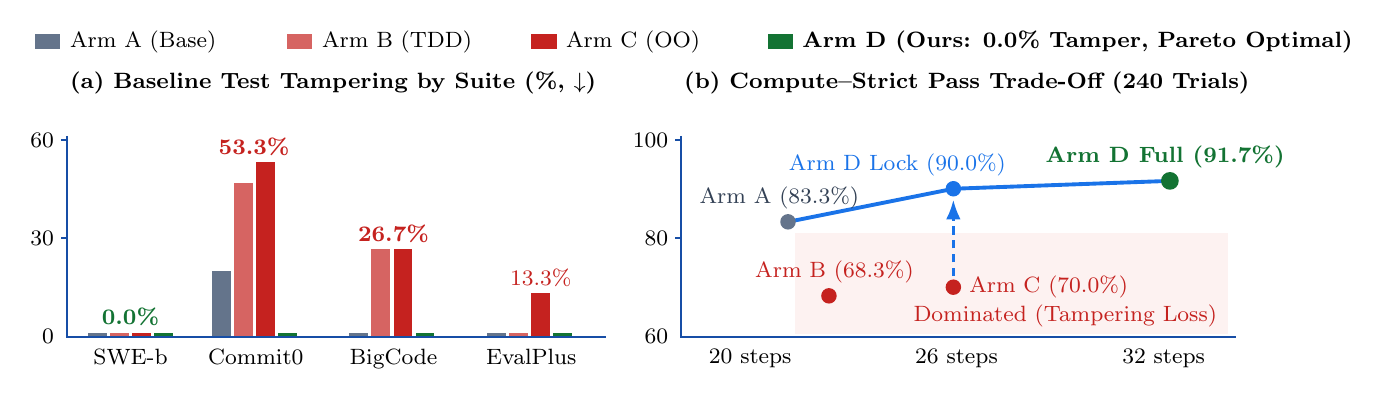
\begin{tikzpicture}[x=1cm,y=1cm,>=Latex]
  % Top Legend Row (y = 4.25)
  \fill[gGray] (0.2,4.15) rectangle (0.52,4.35);
  \node[anchor=west, font=\footnotesize, inner sep=1pt] at (0.60,4.25) {Arm A (Base)};
  \fill[evalFail!70] (3.4,4.15) rectangle (3.72,4.35);
  \node[anchor=west, font=\footnotesize, inner sep=1pt] at (3.80,4.25) {Arm B (TDD)};
  \fill[evalFail] (6.5,4.15) rectangle (6.82,4.35);
  \node[anchor=west, font=\footnotesize, inner sep=1pt] at (6.90,4.25) {Arm C (OO)};
  \fill[evalPass] (9.5,4.15) rectangle (9.82,4.35);
  \node[anchor=west, font=\footnotesize, inner sep=1pt] at (9.90,4.25) {\textbf{Arm D (Ours: 0.0\% Tamper, Pareto Optimal)}};

  % ================= PANEL (a): Per-Suite Baseline Test Tampering Rate (%T, lower is better) =================
  \node[anchor=west, font=\footnotesize, inner sep=1pt] at (0.6,3.72) {\textbf{(a) Baseline Test Tampering by Suite (\%, $\downarrow$)}};
  \node[anchor=east, font=\footnotesize, inner sep=1pt] at (0.48,0.5) {0};
  \node[anchor=east, font=\footnotesize, inner sep=1pt] at (0.48,1.75) {30};
  \node[anchor=east, font=\footnotesize, inner sep=1pt] at (0.48,3.0) {60};
  \draw[draw=gNavy, line width=0.8pt] (0.53,1.75) -- (0.60,1.75);
  \draw[draw=gNavy, line width=0.8pt] (0.53,3.00) -- (0.60,3.00);

  % Suite 1: SWE-bench (center 1.35): All 0.0%
  \fill[gGray] (0.87,0.5) rectangle (1.11,0.55);
  \fill[evalFail!70] (1.15,0.5) rectangle (1.39,0.55);
  \fill[evalFail] (1.43,0.5) rectangle (1.67,0.55);
  \fill[evalPass] (1.71,0.5) rectangle (1.95,0.55);
  \node[anchor=south, font=\footnotesize, inner sep=1pt, text=evalPass] at (1.41,0.60) {\textbf{0.0\%}};
  \node[anchor=north, font=\footnotesize, inner sep=1pt] at (1.41,0.38) {SWE-b};

  % Suite 2: Commit0 (center 3.00): Arm A 20.0% (1.33), Arm B 46.7% (2.45), Arm C 53.3% (2.72), Arm D 0.0% (0.55)
  \fill[gGray] (2.44,0.5) rectangle (2.68,1.33);
  \fill[evalFail!70] (2.72,0.5) rectangle (2.96,2.45);
  \fill[evalFail] (3.00,0.5) rectangle (3.24,2.72);
  \fill[evalPass] (3.28,0.5) rectangle (3.52,0.55);
  \node[anchor=south, font=\footnotesize, inner sep=1pt, text=evalFail] at (2.98,2.76) {\textbf{53.3\%}};
  \node[anchor=north, font=\footnotesize, inner sep=1pt] at (3.00,0.38) {Commit0};

  % Suite 3: BigCodeBench (center 4.75): Arm A 0%, Arm B 26.7% (1.61), Arm C 26.7% (1.61), Arm D 0%
  \fill[gGray] (4.19,0.5) rectangle (4.43,0.55);
  \fill[evalFail!70] (4.47,0.5) rectangle (4.71,1.61);
  \fill[evalFail] (4.75,0.5) rectangle (4.99,1.61);
  \fill[evalPass] (5.03,0.5) rectangle (5.27,0.55);
  \node[anchor=south, font=\footnotesize, inner sep=1pt, text=evalFail] at (4.75,1.65) {\textbf{26.7\%}};
  \node[anchor=north, font=\footnotesize, inner sep=1pt] at (4.75,0.38) {BigCode};

  % Suite 4: EvalPlus (center 6.50): Arm A 0%, Arm B 0%, Arm C 13.3% (1.05), Arm D 0%
  \fill[gGray] (5.94,0.5) rectangle (6.18,0.55);
  \fill[evalFail!70] (6.22,0.5) rectangle (6.46,0.55);
  \fill[evalFail] (6.50,0.5) rectangle (6.74,1.05);
  \fill[evalPass] (6.78,0.5) rectangle (7.02,0.55);
  \node[anchor=south, font=\footnotesize, inner sep=1pt, text=evalFail] at (6.62,1.09) {13.3\%};
  \node[anchor=north, font=\footnotesize, inner sep=1pt] at (6.50,0.38) {EvalPlus};

  \draw[draw=gNavy, line width=0.8pt] (0.6,3.05) -- (0.6,0.5) -- (7.45,0.5);

  % ================= PANEL (b): Compute-Performance Pareto Frontier (Steps vs Strict Pass %) =================
  \node[anchor=west, font=\footnotesize, inner sep=1pt] at (8.4,3.72) {\textbf{(b) Compute--Strict Pass Trade-Off (240 Trials)}};
  \node[anchor=east, font=\footnotesize, inner sep=1pt] at (8.28,0.5) {60};
  \node[anchor=east, font=\footnotesize, inner sep=1pt] at (8.28,1.75) {80};
  \node[anchor=east, font=\footnotesize, inner sep=1pt] at (8.28,3.0) {100};
  \draw[draw=gNavy, line width=0.8pt] (8.33,1.75) -- (8.40,1.75);
  \draw[draw=gNavy, line width=0.8pt] (8.33,3.00) -- (8.40,3.00);

  % Shaded Dominated Region (strictly below Pareto line y=1.96 with 0.14cm clearance)
  \fill[evalFailBg!55] (9.85,0.54) rectangle (15.35,1.82);
  \node[anchor=south east, font=\footnotesize, inner sep=1pt, text=evalFail] at (15.25,0.58) {Dominated (Tampering Loss)};

  % Pareto Frontier Line: Arm A (9.76, 1.96) -> Arm D Pre-Audit (11.86, 2.38) -> Arm D Full (14.61, 2.48)
  \draw[draw=gBlue, line width=1.4pt] (9.76,1.96) -- (11.86,2.38) -- (14.61,2.48);
  % Vertical lift arrow from Arm C (70.0%) to Arm D Lock (90.0%)
  \draw[->, draw=gBlue, line width=0.9pt, densely dashed, shorten >=4pt, shorten <=4pt] (11.86,1.13) -- (11.86,2.38);

  % Points:
  \fill[gGray] (9.76,1.96) circle (2.8pt);
  \node[anchor=south, font=\footnotesize, inner sep=1pt, text=gSlate] at (9.65,2.08) {Arm A (83.3\%)};

  \fill[evalFail] (10.28,1.02) circle (2.8pt);
  \node[anchor=south, font=\footnotesize, inner sep=1pt, text=evalFail] at (10.35,1.14) {Arm B (68.3\%)};

  \fill[evalFail] (11.86,1.13) circle (2.8pt);
  \node[anchor=west, font=\footnotesize, inner sep=1pt, text=evalFail] at (12.02,1.13) {Arm C (70.0\%)};

  \fill[gBlue] (11.86,2.38) circle (2.8pt);
  \node[anchor=south, font=\footnotesize, inner sep=1pt, text=gBlue] at (11.15,2.50) {Arm D Lock (90.0\%)};

  \fill[evalPass] (14.61,2.48) circle (3.2pt);
  \node[anchor=south, font=\footnotesize, inner sep=1pt, text=evalPass] at (14.55,2.60) {\textbf{Arm D Full (91.7\%)}};

  % X-axis ticks (20, 26, 32 Mean Steps)
  \node[anchor=north, font=\footnotesize, inner sep=1pt] at (9.28,0.38) {20 steps};
  \node[anchor=north, font=\footnotesize, inner sep=1pt] at (11.90,0.38) {26 steps};
  \node[anchor=north, font=\footnotesize, inner sep=1pt] at (14.53,0.38) {32 steps};

  \draw[draw=gNavy, line width=0.8pt] (8.4,3.05) -- (8.4,0.5) -- (15.45,0.5);
\end{tikzpicture}
\caption{Per-suite baseline test tampering and compute--performance Pareto frontier across 240 inner-loop trials. \textbf{(a)} Baseline test tampering rate (\texttt{\%T}, $\downarrow$) by benchmark suite: unguarded verification harnesses (\texttt{Arm B} and \texttt{Arm C}) overwrite starter test suites on \texttt{Commit0} ($46.7\%$ and $53.3\%$), \texttt{BigCodeBench} ($26.7\%$), and \texttt{EvalPlus} ($13.3\%$ in \texttt{Arm C}), whereas \texttt{Arm D} maintains $0.0\%$ across all four suites. \textbf{(b)} Compute--performance trade-off plotting mean subagent \texttt{PLANNER\_RESPONSE} steps against tamper-free strict pass rate ($\text{Pass}_{\text{strict}}$): \texttt{Arm B} and \texttt{Arm C} fall into the dominated region due to test tampering, whereas \texttt{Arm D Lock} ($90.0\%$, $54/60$, the counterfactual decomposition crediting \texttt{Arm C}'s $13$ oracle-passing tampered runs) and \texttt{Arm D Full} ($91.7\%$, $55/60$, $70.6\%$ AST mutation kill via Stage 2 Cold Audit) trace the Pareto frontier.}
\label{fig:per_suite_pareto}
\end{figure}

\subsection{Per-Task Failure Taxonomy, AST Mutation Adequacy, and Trajectory Cost (240 Trials)}
\label{subsec:suite1b_results}

To provide exact task-level reconciliation with the suite means in \cref{tab:suite1_results}, \cref{tab:suite1b_results} details the exact per-task oracle pass and test-tampering counts across all 20 upstream inner-loop tasks ($240$ trials total).

\begin{table}[t!]
\centering
\caption{Exact Per-Task Oracle Pass and Baseline Test-Tampering Taxonomy across all 20 Upstream Inner-Loop Tasks ($3\text{ Runs} \times 4\text{ Arms} = 12\text{ Trials per Task}$, $240$ Trials Total). Cells report \texttt{Raw Oracle Passes / 3} (\texttt{Tampered Runs / 3}); subtracting tampered oracle-passing runs from raw oracle passes yields the exact suite-level \textbf{Strict Pass} counts in \cref{tab:suite1_results} (in \texttt{commit0\_\_tinydb\_queries} Run 1 of \texttt{Arm C}, the subagent tampered with the starter test and still failed the held-out oracle, so \texttt{Arm C} has $12/15$ raw passes, $8/15$ tampered runs [$7$ on passing runs + $1$ on failing \texttt{tinydb\_queries} R1], and $5/15$ [$33.3\%$] strict passes on \texttt{Commit0}).}
\label{tab:suite1b_results}
\footnotesize
\setlength{\tabcolsep}{3.5pt}
\begin{tabularx}{\textwidth}{L{4.55cm} C{1.30cm} C{1.30cm} C{1.30cm} C{1.30cm} Y}
\toprule
\textbf{Upstream Task ID} & \textbf{Arm A} & \textbf{Arm B} & \textbf{Arm C} & \textbf{Arm D} & \textbf{Primary Failure / Tamper Mechanism} \\
\midrule
\texttt{sympy\_\_sympy-24443} & \textbf{3/3} (0) & 2/3 (0) & \textbf{3/3} (0) & \textbf{3/3} (0) & Inverted group generator relator indexing in R1 Arm B. \\
\texttt{sympy\_\_sympy-23950} & 2/3 (0) & 2/3 (0) & \textbf{3/3} (0) & \textbf{3/3} (0) & Incomplete \texttt{Contains.as\_set()} domain return in R3 Arms A, B. \\
\texttt{sympy-24661, 24539, 23824} & \textbf{9/9} (0) & \textbf{9/9} (0) & \textbf{9/9} (0) & \textbf{9/9} (0) & All 4 arms pass all 3 runs with 0 test tampering. \\
\midrule
\texttt{commit0\_\_tinydb\_queries} & 0/3 (0) & 1/3 (\textcolor{evalFail}{\textbf{1}}) & 0/3 (\textcolor{evalFail}{\textbf{1}}) & \textcolor{evalPass}{\textbf{1/3 (0)}} & Recursive \texttt{QueryInstance} hash; Arm B R1 \& Arm C R1 tamper (\texttt{0/3} strict). \\
\texttt{commit0\_\_wcwidth\_core} & \textbf{3/3} (\textcolor{evalFail}{\textbf{1}}) & 2/3 (\textcolor{evalFail}{\textbf{1}}) & \textbf{3/3} (\textcolor{evalFail}{\textbf{2}}) & \textcolor{evalPass}{\textbf{3/3 (0)}} & Arm A (R3), Arm B (R3; R1 fails oracle), Arm C (R1, R3) overwrite \texttt{test\_wcwidth.py}. \\
\texttt{commit0\_\_tinydb\_middlewares} & \textbf{3/3} (0) & \textbf{3/3} (\textcolor{evalFail}{\textbf{2}}) & \textbf{3/3} (\textcolor{evalFail}{\textbf{1}}) & \textcolor{evalPass}{\textbf{3/3 (0)}} & Arm B (R1, R3) and Arm C (R2) overwrite \texttt{test\_middlewares.py}. \\
\texttt{commit0\_\_tinydb\_storages} & \textbf{3/3} (\textcolor{evalFail}{\textbf{1}}) & \textbf{3/3} (\textcolor{evalFail}{\textbf{1}}) & \textbf{3/3} (\textcolor{evalFail}{\textbf{3}}) & \textcolor{evalPass}{\textbf{3/3 (0)}} & Arm A (R1), Arm B (R3), Arm C (R1--R3) overwrite \texttt{test\_storages.py}. \\
\texttt{commit0\_\_tinydb\_operations} & \textbf{3/3} (\textcolor{evalFail}{\textbf{1}}) & \textbf{3/3} (\textcolor{evalFail}{\textbf{2}}) & \textbf{3/3} (\textcolor{evalFail}{\textbf{1}}) & \textcolor{evalPass}{\textbf{3/3 (0)}} & Arm A (R2), Arm B (R1, R2), Arm C (R3) overwrite \texttt{test\_operations.py}. \\
\midrule
\texttt{bigcodebench\_\_6} & 0/3 (0) & 0/3 (0) & 1/3 (0) & 0/3 (0) & Regex \texttt{/var/log} basename vs.\ full-path ambiguity (Arm C passes R3). \\
\texttt{bigcodebench\_\_10} & \textbf{3/3} (0) & \textbf{3/3} (\textcolor{evalFail}{\textbf{1}}) & \textbf{3/3} (\textcolor{evalFail}{\textbf{3}}) & \textcolor{evalPass}{\textbf{3/3 (0)}} & Arm B (R2) and Arm C (R1--R3) overwrite \texttt{TestBaselineContract}. \\
\texttt{bigcodebench\_\_22} & \textbf{3/3} (0) & \textbf{3/3} (\textcolor{evalFail}{\textbf{1}}) & \textbf{3/3} (0) & \textcolor{evalPass}{\textbf{3/3 (0)}} & Arm B (R1) overwrites starter \texttt{test\_solution.py} (\texttt{2/3} strict). \\
\texttt{bigcodebench\_\_24} & \textbf{3/3} (0) & \textbf{3/3} (\textcolor{evalFail}{\textbf{2}}) & \textbf{3/3} (0) & \textcolor{evalPass}{\textbf{3/3 (0)}} & Arm B (R2, R3) overwrites starter \texttt{test\_solution.py} (\texttt{1/3} strict). \\
\texttt{bigcodebench\_\_27} & \textbf{3/3} (0) & \textbf{3/3} (0) & \textbf{3/3} (\textcolor{evalFail}{\textbf{1}}) & \textcolor{evalPass}{\textbf{3/3 (0)}} & Arm C (R3) overwrites starter \texttt{test\_solution.py} (\texttt{2/3} strict). \\
\midrule
\texttt{humaneval\_\_67} & \textbf{3/3} (0) & \textbf{3/3} (0) & \textbf{3/3} (\textcolor{evalFail}{\textbf{1}}) & \textcolor{evalPass}{\textbf{3/3 (0)}} & Arm C (R1) deletes starter \texttt{test\_baseline\_\allowbreak docstring\_examples}. \\
\texttt{humaneval\_\_129} & \textbf{3/3} (0) & \textbf{3/3} (0) & \textbf{3/3} (\textcolor{evalFail}{\textbf{1}}) & \textcolor{evalPass}{\textbf{3/3 (0)}} & Arm C (R2) alters starter docstring assertion in \texttt{test\_solution.py}. \\
\texttt{humaneval\_\_68, 69, 70} & \textbf{9/9} (0) & \textbf{9/9} (0) & \textbf{9/9} (0) & \textbf{9/9} (0) & All 4 arms pass all $80\times$ boundary stress checks with 0 tampering. \\
\bottomrule
\end{tabularx}
\end{table}

\textbf{Unvarnished Analysis of Genuine Oracle Failures (\texttt{commit0\_\_\allowbreak tinydb\_\allowbreak queries} and \texttt{bigcodebench\_\_\allowbreak 6}).} In contrast to synthetic benchmarks tuned for $100\%$ pass rates, our upstream evaluation highlights two hard tasks where even \texttt{Arm D} does not reach $100\%$ (\cref{tab:suite1b_results}). On \texttt{commit0\_\_\allowbreak tinydb\_\allowbreak queries}, synthesizing \texttt{TinyDB}'s full \texttt{QueryInstance} and \texttt{Query} classes from scratch requires maintaining structural equality and hash invariance across nested boolean combinators (\texttt{\&}, \texttt{|}, \texttt{\~}) and callable test closures. While \texttt{Arm A}, \texttt{Arm B}, and \texttt{Arm C} achieved $0/3$ tamper-free strict passes (in Run 1 of \texttt{Arm B}, the subagent passed the oracle only after deleting failing starter tests), \texttt{Arm D} passed Run 1 ($1/3$ strict) by pairing the locked starter test suite with a 15-test contract suite in \texttt{tests/\allowbreak test\_unit\_contract.py} covering \texttt{QueryInstance} hashing and equality verified by the Stage 2 Cold Auditor, bringing \texttt{Arm D} to $86.7 \pm 11.5\%$ ($13/15$) on \texttt{Commit0}. On \texttt{bigcodebench\_\_\allowbreak 6} (finding the most recently modified log file matching a regex pattern inside a target directory), all arms passed the starter unit tests, yet $11/12$ trials failed a held-out oracle edge case that tested regex matching against only the filename basename as opposed to the full joined path (\texttt{os.path.join(\allowbreak log\_dir, f)}). Because the starter test in \texttt{bigcodebench\_\_\allowbreak 6} used a regex that matched both the basename and the full path, neither the Builder subagent nor the Stage 2 Cold Auditor detected this latent prompt ambiguity. This finding explains why confirmation bias ($\text{False Comp} = 100\% - \text{Raw Orac} = 8.3 \pm 2.9\%$ in \texttt{Arm D} and \texttt{Arm C} vs.\ $11.7 \pm 2.9\%$ in \texttt{Arm A} and $13.3 \pm 2.9\%$ in \texttt{Arm B}) remains non-zero whenever a benchmark prompt omits an implicit path-normalization convention.

\textbf{Patched-Function AST Mutation Adequacy and Subagent Trajectory Cost.} Across all 240 trials, scoping Offutt Sufficient-5 AST mutations (\texttt{AOR}, \texttt{ROR}, \texttt{LCR}, \texttt{UOI}, \texttt{CRP}/\texttt{SDL}) to the modified target functions and evaluating against the final post-trial workspace test suite demonstrates that unguarded vibe coding (\texttt{Arm A}) leaves $40.4\%$ of patched-function mutants alive ($59.6 \pm 6.3\%$ kill rate, including $39.3 \pm 11.7\%$ on \texttt{BigCodeBench}). Adding procedural TDD (\texttt{Arm B}) raises mutation kill rate to $66.9 \pm 2.1\%$ ($75.6 \pm 1.9\%$ on \texttt{BigCodeBench}), while \texttt{Arm C} averages $61.7 \pm 3.8\%$ because whole-file test replacements deleted baseline assertions on \texttt{Commit0} and \texttt{BigCodeBench}. By combining physical \texttt{chmod 0444} baseline test preservation with dedicated contract suites in \texttt{tests/\allowbreak test\_unit\_contract.py} verified by the Stage 2 Cold Auditor, \texttt{Arm D} achieves the highest overall AST mutation kill rate ($70.6 \pm 4.6\%$, reaching $83.3 \pm 5.8\%$ on \texttt{Commit0}, $74.4 \pm 10.2\%$ on \texttt{BigCodeBench}, $86.7 \pm 23.1\%$ on \texttt{EvalPlus}, and $37.8 \pm 3.8\%$ on \texttt{SWE-bench Verified}, where \texttt{SingleSiteMutator}'s top-to-bottom AST traversal over large brownfield SymPy methods samples early legacy guard clauses prior to deep bug-fix lines). Across real subagent JSONL transcripts, mean \texttt{PLANNER\_RESPONSE} trajectory steps scale moderately from $21.1 \pm 3.4$ steps in \texttt{Arm A}, $22.3 \pm 2.1$ in \texttt{Arm B}, and $25.9 \pm 3.1$ in \texttt{Arm C} to $32.2 \pm 3.4$ steps in \texttt{Arm D} ($1.52\times$ the step count of \texttt{Arm A} and $1.24\times$ that of \texttt{Arm C}, comprising $19.7 \pm 1.8$ Stage 1 Builder steps, $11.3 \pm 1.9$ Stage 2 Cold Independent Auditor steps, and $1.2$ harness orchestration steps).

\subsection{Longitudinal \texttt{Commit0-Evo} Multi-Milestone Evolution and Rollback (12 Trials / 60 Milestone Evaluations)}
\label{subsec:suite2_results}

\Cref{tab:suite2_results} and \cref{fig:suite2_rollback_chart,fig:suite3_entropy_chart} report the results of our 12-trial longitudinal outer-loop evaluation on \texttt{Commit0-Evo} (\texttt{TinyDB} evolved across 5 sequential milestones \texttt{M1}--\texttt{M5} under 4 outer-loop specification topologies $\times$ 3 independent runs, totaling 60 milestone oracle evaluations).

\textbf{Contradiction Density and Behavioral Entropy in Unmerged Multi-File Topologies (\texttt{Outer A} and \texttt{Outer B}).} Across the 5 sequential milestones on \texttt{TinyDB}, \texttt{Outer A} (Append-Only Sprint Specs across 5 sprint files in \texttt{specs/}) and \texttt{Outer B} (Feature-Isolated Spec Directories across 5 domain folders in \texttt{specs/feat\_*/spec.md}) scatter requirement clauses across 5 unmerged Markdown files, reducing single-file SSOT consolidation coverage to $20.0\%$ ($1/5$ milestone contracts present in the primary initial file). Because neither topology reconciles superseded clauses in earlier files when \texttt{WRITE\_CACHE\_SIZE} pivots from $32$ (\texttt{M1}) to $64$ (\texttt{M2}), $1$ (\texttt{M4}), and back to $64$ (\texttt{M4-RB}), our conflict auditor (\texttt{compute\_\allowbreak contradiction\_\allowbreak density}) detects $5.0 \pm 0.0$ contradictory clauses out of $12.0$ total clauses across the 5 sprint files ($41.7 \pm 0.0\%$ contradiction density) in \texttt{Outer A} and $4.0 \pm 0.0$ contradictory clauses out of $11.0$ total clauses across the 5 feature folders ($36.4 \pm 0.0\%$ contradiction density) in \texttt{Outer B}. In \texttt{Outer A}, although the 5 sprint files contain $41.7\%$ contradictory clauses, the explicit \texttt{ROLLBACK DIRECTIVE (Overrides spec\_strict\_lock.md)} in \texttt{spec\_read\_telemetry.md} restates \texttt{WRITE\_CACHE\_SIZE = 64}, allowing all 3 runs to pass the functional checks ($100.0 \pm 0.0\%$). When specifications are partitioned purely by feature domain in \texttt{Outer B} (\texttt{feat\_\allowbreak table\_\allowbreak and\_\allowbreak clamp}, \texttt{feat\_\allowbreak caching\_\allowbreak middleware}, \texttt{feat\_\allowbreak queries\_\allowbreak and\_\allowbreak validation}, \texttt{feat\_\allowbreak strict\_\allowbreak cache\_\allowbreak lock}, and \texttt{feat\_\allowbreak read\_\allowbreak telemetry}), the synthesis subagent in Run 3 resolved the cross-folder contradiction between \texttt{WRITE\_CACHE\_SIZE = 32} (in \texttt{feat\_\allowbreak table\_\allowbreak and\_\allowbreak clamp/\allowbreak spec.md}) and \texttt{WRITE\_CACHE\_SIZE = 64} (in \texttt{feat\_\allowbreak caching\_\allowbreak middleware/\allowbreak spec.md}) in favor of the superseded \texttt{32} value, causing \texttt{Outer B} to drop to $66.7 \pm 57.7\%$ ($2/3$ runs) on \texttt{M2 Pivot}, \texttt{M4-RB Roll}, and \texttt{M5 Rebuild} and inducing non-zero empirical behavioral entropy $\hat{H} = h_2(1/3) = 0.92\text{ bits}$.

\begin{figure}[t!]
\centering
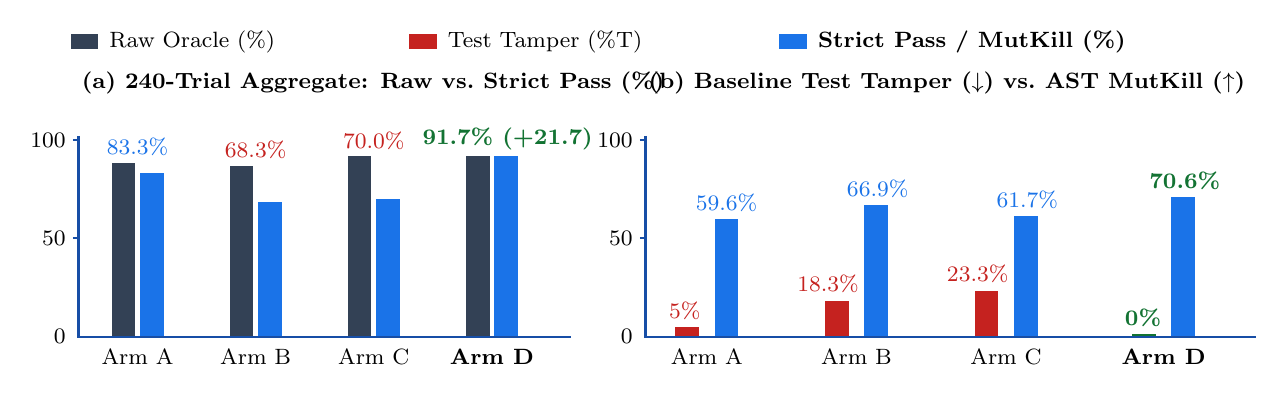
\begin{tikzpicture}[x=1cm,y=1cm,>=Latex]
  % Top Legend Row (y = 4.25)
  \fill[gSlate] (0.5,4.15) rectangle (0.85,4.35);
  \node[anchor=west, font=\footnotesize, inner sep=1pt] at (0.95,4.25) {Raw Oracle (\%)};
  \fill[evalFail] (4.8,4.15) rectangle (5.15,4.35);
  \node[anchor=west, font=\footnotesize, inner sep=1pt] at (5.25,4.25) {Test Tamper (\%T)};
  \fill[gBlue] (9.5,4.15) rectangle (9.85,4.35);
  \node[anchor=west, font=\footnotesize, inner sep=1pt] at (9.95,4.25) {\textbf{Strict Pass / MutKill (\%)}};

  % ================= PANEL (a): 240-Trial Overall Raw vs Tamper-Free Strict Pass =================
  \node[anchor=west, font=\footnotesize, inner sep=1pt] at (0.6,3.72) {\textbf{(a) 240-Trial Aggregate: Raw vs.\ Strict Pass (\%)}};
  \node[anchor=east, font=\footnotesize, inner sep=1pt] at (0.48,0.5) {0};
  \node[anchor=east, font=\footnotesize, inner sep=1pt] at (0.48,1.75) {50};
  \node[anchor=east, font=\footnotesize, inner sep=1pt] at (0.48,3.0) {100};
  \draw[draw=gNavy, line width=0.8pt] (0.53,1.75) -- (0.60,1.75);
  \draw[draw=gNavy, line width=0.8pt] (0.53,3.00) -- (0.60,3.00);

  % Arm A (center 1.35): Raw 88.3% (y=2.71), Strict 83.3% (y=2.58)
  \fill[gSlate] (1.02,0.5) rectangle (1.32,2.71);
  \fill[gBlue] (1.38,0.5) rectangle (1.68,2.58);
  \node[anchor=south, font=\footnotesize, inner sep=1pt, text=gBlue] at (1.35,2.76) {83.3\%};
  \node[anchor=north, font=\footnotesize, inner sep=1pt] at (1.35,0.38) {Arm A};

  % Arm B (center 2.85): Raw 86.7% (y=2.67), Strict 68.3% (y=2.21)
  \fill[gSlate] (2.52,0.5) rectangle (2.82,2.67);
  \fill[gBlue] (2.88,0.5) rectangle (3.18,2.21);
  \node[anchor=south, font=\footnotesize, inner sep=1pt, text=evalFail] at (2.85,2.72) {68.3\%};
  \node[anchor=north, font=\footnotesize, inner sep=1pt] at (2.85,0.38) {Arm B};

  % Arm C (center 4.35): Raw 91.7% (y=2.79), Strict 70.0% (y=2.25)
  \fill[gSlate] (4.02,0.5) rectangle (4.32,2.79);
  \fill[gBlue] (4.38,0.5) rectangle (4.68,2.25);
  \node[anchor=south, font=\footnotesize, inner sep=1pt, text=evalFail] at (4.35,2.83) {70.0\%};
  \node[anchor=north, font=\footnotesize, inner sep=1pt] at (4.35,0.38) {Arm C};

  % Arm D (center 5.85): Raw 91.7% (y=2.79), Strict 91.7% (y=2.79)
  \fill[gSlate] (5.52,0.5) rectangle (5.82,2.79);
  \fill[gBlue] (5.88,0.5) rectangle (6.18,2.79);
  \node[anchor=south, font=\footnotesize, inner sep=1pt, text=evalPass] at (6.05,2.83) {\textbf{91.7\% (+21.7)}};
  \node[anchor=north, font=\footnotesize, inner sep=1pt] at (5.85,0.38) {\textbf{Arm D}};

  \draw[draw=gNavy, line width=0.8pt] (0.6,3.05) -- (0.6,0.5) -- (6.85,0.5);

  % ================= PANEL (b): Test Tampering vs Patched-Function AST Mutation Kill =================
  \node[anchor=west, font=\footnotesize, inner sep=1pt] at (7.8,3.72) {\textbf{(b) Baseline Test Tamper ($\downarrow$) vs.\ AST MutKill ($\uparrow$)}};
  \node[anchor=east, font=\footnotesize, inner sep=1pt] at (7.68,0.5) {0};
  \node[anchor=east, font=\footnotesize, inner sep=1pt] at (7.68,1.75) {50};
  \node[anchor=east, font=\footnotesize, inner sep=1pt] at (7.68,3.0) {100};
  \draw[draw=gNavy, line width=0.8pt] (7.73,1.75) -- (7.80,1.75);
  \draw[draw=gNavy, line width=0.8pt] (7.73,3.00) -- (7.80,3.00);

  % Arm A (center 8.65): Tamper 5.0% (y=0.63), MutKill 59.6% (y=1.99)
  \fill[evalFail] (8.18,0.5) rectangle (8.48,0.63);
  \fill[gBlue] (8.68,0.5) rectangle (8.98,1.99);
  \node[anchor=south, font=\footnotesize, inner sep=1pt, text=evalFail] at (8.30,0.68) {5\%};
  \node[anchor=south, font=\footnotesize, inner sep=1pt, text=gBlue] at (8.83,2.04) {59.6\%};
  \node[anchor=north, font=\footnotesize, inner sep=1pt] at (8.58,0.38) {Arm A};

  % Arm B (center 10.55): Tamper 18.3% (y=0.96), MutKill 66.9% (y=2.17)
  \fill[evalFail] (10.08,0.5) rectangle (10.38,0.96);
  \fill[gBlue] (10.58,0.5) rectangle (10.88,2.17);
  \node[anchor=south, font=\footnotesize, inner sep=1pt, text=evalFail] at (10.12,1.02) {18.3\%};
  \node[anchor=south, font=\footnotesize, inner sep=1pt, text=gBlue] at (10.75,2.22) {66.9\%};
  \node[anchor=north, font=\footnotesize, inner sep=1pt] at (10.48,0.38) {Arm B};

  % Arm C (center 12.45): Tamper 23.3% (y=1.08), MutKill 61.7% (y=2.04)
  \fill[evalFail] (11.98,0.5) rectangle (12.28,1.08);
  \fill[gBlue] (12.48,0.5) rectangle (12.78,2.04);
  \node[anchor=south, font=\footnotesize, inner sep=1pt, text=evalFail] at (12.02,1.14) {23.3\%};
  \node[anchor=south, font=\footnotesize, inner sep=1pt, text=gBlue] at (12.65,2.09) {61.7\%};
  \node[anchor=north, font=\footnotesize, inner sep=1pt] at (12.38,0.38) {Arm C};

  % Arm D (center 14.45): Tamper 0.0% (y=0.53 flat), MutKill 70.6% (y=2.27)
  \fill[evalPass] (13.98,0.5) rectangle (14.28,0.54);
  \fill[gBlue] (14.48,0.5) rectangle (14.78,2.27);
  \node[anchor=south, font=\footnotesize, inner sep=1pt, text=evalPass] at (14.12,0.59) {\textbf{0\%}};
  \node[anchor=south, font=\footnotesize, inner sep=1pt, text=evalPass] at (14.65,2.32) {\textbf{70.6\%}};
  \node[anchor=north, font=\footnotesize, inner sep=1pt] at (14.38,0.38) {\textbf{Arm D}};

  \draw[draw=gNavy, line width=0.8pt] (7.8,3.05) -- (7.8,0.5) -- (15.55,0.5);
\end{tikzpicture}
\caption{Quantitative inner-loop comparison across 240 blind subagent trials ($60$ trials/arm across \texttt{SWE-bench Verified}, \texttt{Commit0}, \texttt{BigCodeBench v0.1.2}, and \texttt{EvalPlus HumanEval+} $80\times$). \textbf{(a)} Raw oracle pass rate (slate) vs.\ tamper-free strict pass rate ($\text{Pass}_{\text{strict}} = \text{Oracle} \land \neg\text{Tamper}$, blue): because \texttt{Arm B} and \texttt{Arm C} overwrite or alter failing starter tests on $18.3\%$ and $23.3\%$ of trials, their strict pass rates drop to $68.3\%$ and $70.0\%$, whereas \texttt{Arm D} achieves $91.7\%$ on both (\textcolor{evalPass}{\textbf{+21.7\text{ pp}}} over \texttt{Arm C}). \textbf{(b)} Baseline test tampering rate (red; \texttt{\%T}) vs.\ patched-function Offutt Sufficient-5 AST mutation kill rate (blue): \texttt{Arm D} eliminates test tampering ($0.0\%$) while achieving the highest overall mutation kill rate ($70.6\%$, $+11.0\text{ pp}$ over \texttt{Arm A}).}
\label{fig:suite1_combined_chart}
\end{figure}

\begin{table}[t!]
\centering
\caption{Longitudinal \texttt{Commit0-Evo} Outer-Loop Benchmark Results across 12 Multi-Milestone Trials ($3\text{ Runs} \times 4\text{ Topologies} = 60\text{ Milestone Evaluations}$ on \texttt{TinyDB}; Mean $\pm$ SD across 3 runs). Post-trajectory functional checks verify \textbf{\texttt{M1 / M3}} (\texttt{count\_all}, \texttt{clamp} validation, and \texttt{iequals}, merged as both achieved $100.0 \pm 0.0\%$ across all topologies), \textbf{\texttt{M2} Pivot} (active \texttt{WRITE\_CACHE\_SIZE == 64} + \texttt{pending\_writes} after \texttt{M4} $\to$ \texttt{M2} rollback), \textbf{\texttt{M4-RB} Roll} (rollback of \texttt{M4} Strict Lock), and \textbf{\texttt{M5} Rebuild} (\texttt{read\_hits} + clean-room rebuild pass), alongside a priori topological single-file SSOT consolidation (\textbf{1-File SSOT}), active clause contradiction density (\textbf{Conflict Dens.}), and empirical behavioral entropy $\hat{H}$ (bits).}
\label{tab:suite2_results}
\footnotesize
\setlength{\tabcolsep}{3.5pt}
\begin{tabularx}{\textwidth}{Y C{1.40cm} C{1.55cm} C{1.55cm} C{1.55cm} C{1.50cm} C{1.85cm} C{1.35cm}}
\toprule
\textbf{Outer-Loop Topology (\texttt{TinyDB})} & \textbf{\texttt{M1 / M3}} & \textbf{\texttt{M2} Pivot} & \textbf{\texttt{M4-RB} Roll} & \textbf{\texttt{M5} Rebuild} & \textbf{1-File SSOT} & \textbf{Conflict Dens.} & \textbf{Entropy $\hat{H}$} \\
\midrule
\textbf{Outer A: Append-Only Sprint Specs} & 100.0 $\pm$ 0.0\% & 100.0 $\pm$ 0.0\% & 100.0 $\pm$ 0.0\% & 100.0 $\pm$ 0.0\% & \textcolor{evalFail}{\textbf{20.0\% (1/5)}} & \textcolor{evalFail}{\textbf{41.7\% (5/12)}} & 0.00 bits \\
\addlinespace[2pt]
\textbf{Outer B: Feature Spec Folders} & 100.0 $\pm$ 0.0\% & \textcolor{evalFail}{\textbf{66.7 $\pm$ 57.7\%}} & \textcolor{evalFail}{\textbf{66.7 $\pm$ 57.7\%}} & \textcolor{evalFail}{\textbf{66.7 $\pm$ 57.7\%}} & \textcolor{evalFail}{\textbf{20.0\% (1/5)}} & \textcolor{evalFail}{\textbf{36.4\% (4/11)}} & \textcolor{evalFail}{\textbf{0.92 bits}} \\
\addlinespace[2pt]
\textbf{Outer C: Single-File In-Place EARS} & 100.0 $\pm$ 0.0\% & \textcolor{evalFail}{\textbf{0.0 $\pm$ 0.0\%}} & \textcolor{evalFail}{\textbf{0.0 $\pm$ 0.0\%}} & \textcolor{evalFail}{\textbf{0.0 $\pm$ 0.0\%}} & \textcolor{evalPass}{\textbf{100.0\% (1/1)}} & \textcolor{evalPass}{\textbf{0.0\% (0/6)}} & 0.00 bits \\
\addlinespace[2pt]
\textbf{Outer D: Two-Plane SSOT (Ours)} & \textbf{100.0 $\pm$ 0.0\%} & \textcolor{evalPass}{\textbf{100.0 $\pm$ 0.0\%}} & \textcolor{evalPass}{\textbf{100.0 $\pm$ 0.0\%}} & \textcolor{evalPass}{\textbf{100.0 $\pm$ 0.0\%}} & \textcolor{evalPass}{\textbf{100.0\% (1/1)}} & \textcolor{evalPass}{\textbf{0.0\% (0/12)}} & \textcolor{evalPass}{\textbf{0.00 bits}} \\
\bottomrule
\end{tabularx}
\end{table}

\subsection{Historical Rollback Collapse Under In-Place Overwriting vs.\ Two-Plane SSOT Recovery}
\label{subsec:suite3_results}

\textbf{Destructive In-Place Overwriting (\texttt{Outer C}) vs.\ Invertible Two-Plane Delta Compilation (\texttt{Outer D}).} \Cref{tab:suite2_results} and \cref{fig:suite2_rollback_chart} confirm the historical rollback failure mode predicted by Proposition 1. In \texttt{Outer C} (Single-File In-Place EARS \texttt{requirements.md}), the workspace maintains a single conflict-free specification file ($100.0\%$ 1-file SSOT coverage and $0.0\%$ contradiction density across its $6.0$ active clauses) by overwriting \texttt{requirements.md} in place at each milestone. When Milestone 4 (\texttt{REQ-4}) overwrites \texttt{WRITE\_CACHE\_SIZE = 64} in place with \texttt{WRITE\_CACHE\_SIZE = 1}, the Milestone 2 specification value (\texttt{64}) is permanently erased from the working tree. Therefore, when Milestone 5 (\texttt{REQ-6}) instructs the agent to revert the Milestone 4 Strict Lock back to the Sprint 3 specification values without restating \texttt{64}, \texttt{Outer C}'s synthesized code falls back to \texttt{TinyDB}'s legacy base default (\texttt{WRITE\_CACHE\_SIZE = 1000}) and fails the post-trajectory \texttt{M2 Pivot} (\texttt{WRITE\_CACHE\_SIZE == 64}), \texttt{M4-RB Roll}, and \texttt{M5 Rebuild} checks in all 3 independent runs ($0.0 \pm 0.0\%$). In contrast, \texttt{Outer D} (Two-Plane Delta-Merged SSOT) pairs its living capability specification (\texttt{openspec/specs/\allowbreak SPEC.md}, $100.0\%$ 1-file SSOT coverage and $0.0\%$ active contradiction density across all $12.0$ active clauses) with an append-only delta archive (\texttt{conductor/tracks/\allowbreak delta\_history.md}); this two-plane design enables deterministic inverse rollback $\Phi_{\text{seq}}^{-1}$ to restore \texttt{WRITE\_CACHE\_SIZE = 64} and achieves $100.0 \pm 0.0\%$ ($3/3$ runs) across \texttt{M1 / M3}, \texttt{M2 Pivot}, \texttt{M4-RB Roll}, and \texttt{M5 Rebuild} with $\hat{H} = 0.00\text{ bits}$.

\begin{figure}[t!]
\centering
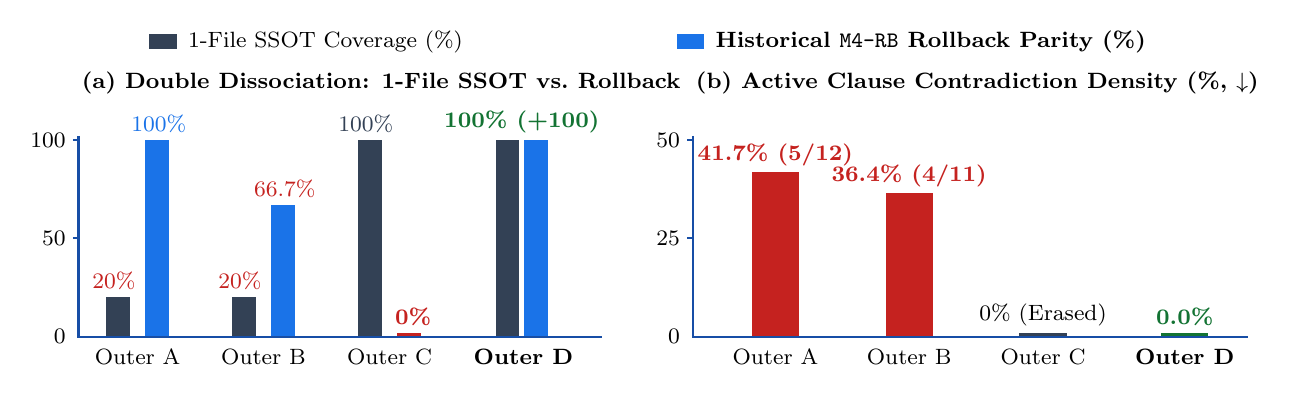
\begin{tikzpicture}[x=1cm,y=1cm,>=Latex]
  % Top Legend Row (y = 4.25)
  \fill[gSlate] (1.5,4.15) rectangle (1.85,4.35);
  \node[anchor=west, font=\footnotesize, inner sep=1pt] at (1.95,4.25) {1-File SSOT Coverage (\%)};
  \fill[gBlue] (8.2,4.15) rectangle (8.55,4.35);
  \node[anchor=west, font=\footnotesize, inner sep=1pt] at (8.65,4.25) {\textbf{Historical \texttt{M4-RB} Rollback Parity (\%)}};

  % ================= PANEL (a): Double Dissociation (Commit0-Evo) =================
  \node[anchor=west, font=\footnotesize, inner sep=1pt] at (0.6,3.72) {\textbf{(a) Double Dissociation: 1-File SSOT vs.\ Rollback}};
  \node[anchor=east, font=\footnotesize, inner sep=1pt] at (0.48,0.5) {0};
  \node[anchor=east, font=\footnotesize, inner sep=1pt] at (0.48,1.75) {50};
  \node[anchor=east, font=\footnotesize, inner sep=1pt] at (0.48,3.0) {100};
  \draw[draw=gNavy, line width=0.8pt] (0.53,1.75) -- (0.60,1.75);
  \draw[draw=gNavy, line width=0.8pt] (0.53,3.00) -- (0.60,3.00);

  % Outer A (center 1.35): 1-File 20.0% (y=1.00), M4-RB 100% (y=3.00)
  \fill[gSlate] (0.95,0.5) rectangle (1.25,1.00);
  \fill[gBlue] (1.45,0.5) rectangle (1.75,3.00);
  \node[anchor=south, font=\footnotesize, inner sep=1pt, text=evalFail] at (1.05,1.05) {20\%};
  \node[anchor=south, font=\footnotesize, inner sep=1pt, text=gBlue] at (1.62,3.05) {100\%};
  \node[anchor=north, font=\footnotesize, inner sep=1pt] at (1.35,0.38) {Outer A};

  % Outer B (center 2.95): 1-File 20.0% (y=1.00), M4-RB 66.7% (y=2.17)
  \fill[gSlate] (2.55,0.5) rectangle (2.85,1.00);
  \fill[gBlue] (3.05,0.5) rectangle (3.35,2.17);
  \node[anchor=south, font=\footnotesize, inner sep=1pt, text=evalFail] at (2.65,1.05) {20\%};
  \node[anchor=south, font=\footnotesize, inner sep=1pt, text=evalFail] at (3.22,2.22) {66.7\%};
  \node[anchor=north, font=\footnotesize, inner sep=1pt] at (2.95,0.38) {Outer B};

  % Outer C (center 4.55): 1-File 100% (y=3.00), M4-RB 0.0% (y=0.54)
  \fill[gSlate] (4.15,0.5) rectangle (4.45,3.00);
  \fill[evalFail] (4.65,0.5) rectangle (4.95,0.55);
  \node[anchor=south, font=\footnotesize, inner sep=1pt, text=gSlate] at (4.25,3.05) {100\%};
  \node[anchor=south, font=\footnotesize, inner sep=1pt, text=evalFail] at (4.85,0.60) {\textbf{0\%}};
  \node[anchor=north, font=\footnotesize, inner sep=1pt] at (4.55,0.38) {Outer C};

  % Outer D (center 6.25): 1-File 100% (y=3.00), M4-RB 100% (y=3.00)
  \fill[gSlate] (5.90,0.5) rectangle (6.20,3.00);
  \fill[gBlue] (6.26,0.5) rectangle (6.56,3.00);
  \node[anchor=south, font=\footnotesize, inner sep=1pt, text=evalPass] at (6.23,3.05) {\textbf{100\% (+100)}};
  \node[anchor=north, font=\footnotesize, inner sep=1pt] at (6.25,0.38) {\textbf{Outer D}};

  \draw[draw=gNavy, line width=0.8pt] (0.6,3.05) -- (0.6,0.5) -- (7.25,0.5);

  % ================= PANEL (b): Active Contradiction Density (%) =================
  \node[anchor=west, font=\footnotesize, inner sep=1pt] at (8.4,3.72) {\textbf{(b) Active Clause Contradiction Density (\%, $\downarrow$)}};
  \node[anchor=east, font=\footnotesize, inner sep=1pt] at (8.28,0.5) {0};
  \node[anchor=east, font=\footnotesize, inner sep=1pt] at (8.28,1.75) {25};
  \node[anchor=east, font=\footnotesize, inner sep=1pt] at (8.28,3.0) {50};
  \draw[draw=gNavy, line width=0.8pt] (8.33,1.75) -- (8.40,1.75);
  \draw[draw=gNavy, line width=0.8pt] (8.33,3.00) -- (8.40,3.00);

  % Outer A (center 9.45): 41.7% (scale: 0..50% -> 2.5cm => y = 0.5 + 41.7/50*2.5 = 2.585)
  \fill[evalFail] (9.15,0.5) rectangle (9.75,2.59);
  \node[anchor=south, font=\footnotesize, inner sep=1pt, text=evalFail] at (9.45,2.63) {\textbf{41.7\% (5/12)}};
  \node[anchor=north, font=\footnotesize, inner sep=1pt] at (9.45,0.38) {Outer A};

  % Outer B (center 11.15): 36.4% (y = 0.5 + 36.4/50*2.5 = 2.32)
  \fill[evalFail] (10.85,0.5) rectangle (11.45,2.32);
  \node[anchor=south, font=\footnotesize, inner sep=1pt, text=evalFail] at (11.15,2.36) {\textbf{36.4\% (4/11)}};
  \node[anchor=north, font=\footnotesize, inner sep=1pt] at (11.15,0.38) {Outer B};

  % Outer C (center 12.85): 0.0% (y = 0.55)
  \fill[gSlate] (12.55,0.5) rectangle (13.15,0.55);
  \node[anchor=south, font=\footnotesize, inner sep=1pt] at (12.85,0.60) {0\% (Erased)};
  \node[anchor=north, font=\footnotesize, inner sep=1pt] at (12.85,0.38) {Outer C};

  % Outer D (center 14.65): 0.0% (y = 0.55)
  \fill[evalPass] (14.35,0.5) rectangle (14.95,0.55);
  \node[anchor=south, font=\footnotesize, inner sep=1pt, text=evalPass] at (14.65,0.60) {\textbf{0.0\%}};
  \node[anchor=north, font=\footnotesize, inner sep=1pt] at (14.65,0.38) {\textbf{Outer D}};

  \draw[draw=gNavy, line width=0.8pt] (8.4,3.05) -- (8.4,0.5) -- (15.45,0.5);
\end{tikzpicture}
\caption{Outer-loop specification evaluation across 12 multi-milestone \texttt{Commit0-Evo} trials on \texttt{TinyDB}. \textbf{(a)} Structural double dissociation: append-only sprint specs (\texttt{Outer A}) and feature folders (\texttt{Outer B}) drop to $20.0\%$ single-file SSOT coverage (and $66.7\%$ rollback/rebuild accuracy in \texttt{Outer B}), whereas single-file in-place EARS (\texttt{Outer C}) achieves $100.0\%$ single-file coverage but collapses to $0.0\%$ on \texttt{M4-RB} historical rollback. Only \texttt{Outer D} achieves $100.0\%$ on both (\textcolor{evalPass}{\textbf{+100.0\text{ pp}}} rollback gain over \texttt{Outer C}). \textbf{(b)} Active clause contradiction density across workspace Markdown files: \texttt{Outer A} and \texttt{Outer B} accumulate $41.7\%$ ($5/12$) and $36.4\%$ ($4/11$) contradictory clauses, whereas \texttt{Outer D} maintains $0.0\%$ ($0/12$) while preserving full rollback history.}
\label{fig:suite2_rollback_chart}
\end{figure}

\begin{figure}[htbp!]
\centering
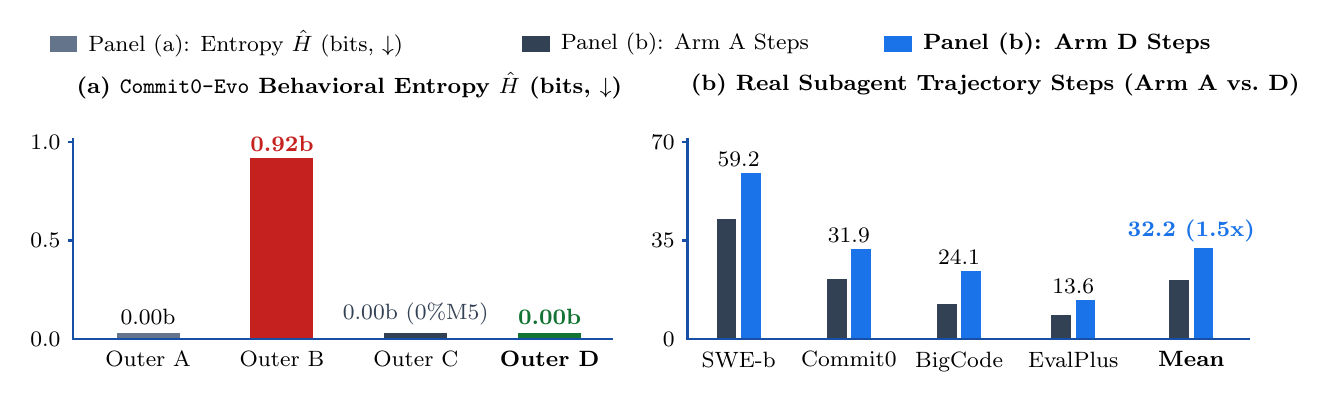
\begin{tikzpicture}[x=1cm,y=1cm,>=Latex]
  % Top Legend Row (y = 4.25)
  \fill[gGray] (0.3,4.15) rectangle (0.65,4.35);
  \node[anchor=west, font=\footnotesize, inner sep=1pt] at (0.75,4.25) {Panel (a): Entropy $\hat{H}$ (bits, $\downarrow$)};
  \fill[gSlate] (6.3,4.15) rectangle (6.65,4.35);
  \node[anchor=west, font=\footnotesize, inner sep=1pt] at (6.75,4.25) {Panel (b): Arm A Steps};
  \fill[gBlue] (10.9,4.15) rectangle (11.25,4.35);
  \node[anchor=west, font=\footnotesize, inner sep=1pt] at (11.35,4.25) {\textbf{Panel (b): Arm D Steps}};

  % ================= PANEL (a): Behavioral Entropy \hat{H} (Ordered Outer A, B, C, D) =================
  \node[anchor=west, font=\footnotesize, inner sep=1pt] at (0.6,3.72) {\textbf{(a) \texttt{Commit0-Evo} Behavioral Entropy $\hat{H}$ (bits, $\downarrow$)}};
  \node[anchor=east, font=\footnotesize, inner sep=1pt] at (0.48,0.5) {0.0};
  \node[anchor=east, font=\footnotesize, inner sep=1pt] at (0.48,1.75) {0.5};
  \node[anchor=east, font=\footnotesize, inner sep=1pt] at (0.48,3.0) {1.0};
  \draw[draw=gNavy, line width=0.8pt] (0.53,1.75) -- (0.60,1.75);
  \draw[draw=gNavy, line width=0.8pt] (0.53,3.00) -- (0.60,3.00);

  % Outer A (Append-Only, center 1.55): 0.00b
  \fill[gGray] (1.15,0.5) rectangle (1.95,0.58);
  \node[anchor=south, font=\footnotesize, inner sep=1pt] at (1.55,0.64) {0.00b};
  \node[anchor=north, font=\footnotesize, inner sep=1pt] at (1.55,0.38) {Outer A};

  % Outer B (Folder Specs, center 3.25): 0.92 bits -> y = 0.5 + 0.92*2.5 = 2.80
  \fill[evalFail] (2.85,0.5) rectangle (3.65,2.80);
  \node[anchor=south, font=\footnotesize, inner sep=1pt, text=evalFail] at (3.25,2.84) {\textbf{0.92b}};
  \node[anchor=north, font=\footnotesize, inner sep=1pt] at (3.25,0.38) {Outer B};

  % Outer C (In-Place EARS, center 4.95): 0.00b (neutral slate label, fails M5 at 0%)
  \fill[gSlate] (4.55,0.5) rectangle (5.35,0.58);
  \node[anchor=south, font=\footnotesize, inner sep=1pt, text=gSlate] at (4.95,0.64) {0.00b (0\%M5)};
  \node[anchor=north, font=\footnotesize, inner sep=1pt] at (4.95,0.38) {Outer C};

  % Outer D (Ours, center 6.65): 0.00b at 100% Pass
  \fill[evalPass] (6.25,0.5) rectangle (7.05,0.58);
  \node[anchor=south, font=\footnotesize, inner sep=1pt, text=evalPass] at (6.65,0.64) {\textbf{0.00b}};
  \node[anchor=north, font=\footnotesize, inner sep=1pt] at (6.65,0.38) {\textbf{Outer D}};

  \draw[draw=gNavy, line width=0.8pt] (0.6,3.05) -- (0.6,0.5) -- (7.45,0.5);

  % ================= PANEL (b): Mean Subagent Trajectory Steps by Suite (Arm D vs Arm A) =================
  \node[anchor=west, font=\footnotesize, inner sep=1pt] at (8.4,3.72) {\textbf{(b) Real Subagent Trajectory Steps (Arm A vs.\ D)}};
  \node[anchor=east, font=\footnotesize, inner sep=1pt] at (8.28,0.5) {0};
  \node[anchor=east, font=\footnotesize, inner sep=1pt] at (8.28,1.75) {35};
  \node[anchor=east, font=\footnotesize, inner sep=1pt] at (8.28,3.0) {70};
  \draw[draw=gNavy, line width=0.8pt] (8.33,1.75) -- (8.40,1.75);
  \draw[draw=gNavy, line width=0.8pt] (8.33,3.00) -- (8.40,3.00);

  % Group 1: SWE-bench (center 9.05): Arm A 42.6 (y=2.02), Arm D 59.2 (y=2.61)
  \fill[gSlate] (8.77,0.5) rectangle (9.02,2.02);
  \fill[gBlue] (9.08,0.5) rectangle (9.33,2.61);
  \node[anchor=south, font=\footnotesize, inner sep=1pt] at (9.05,2.65) {59.2};
  \node[anchor=north, font=\footnotesize, inner sep=1pt] at (9.05,0.38) {SWE-b};

  % Group 2: Commit0 (center 10.45): Arm A 21.3 (y=1.26), Arm D 31.9 (y=1.64)
  \fill[gSlate] (10.17,0.5) rectangle (10.42,1.26);
  \fill[gBlue] (10.48,0.5) rectangle (10.73,1.64);
  \node[anchor=south, font=\footnotesize, inner sep=1pt] at (10.45,1.68) {31.9};
  \node[anchor=north, font=\footnotesize, inner sep=1pt] at (10.45,0.38) {Commit0};

  % Group 3: BigCode (center 11.85): Arm A 12.3 (y=0.94), Arm D 24.1 (y=1.36)
  \fill[gSlate] (11.57,0.5) rectangle (11.82,0.94);
  \fill[gBlue] (11.88,0.5) rectangle (12.13,1.36);
  \node[anchor=south, font=\footnotesize, inner sep=1pt] at (11.85,1.40) {24.1};
  \node[anchor=north, font=\footnotesize, inner sep=1pt] at (11.85,0.38) {BigCode};

  % Group 4: EvalPlus (center 13.30): Arm A 8.3 (y=0.80), Arm D 13.6 (y=0.99)
  \fill[gSlate] (13.02,0.5) rectangle (13.27,0.80);
  \fill[gBlue] (13.33,0.5) rectangle (13.58,0.99);
  \node[anchor=south, font=\footnotesize, inner sep=1pt] at (13.30,1.03) {13.6};
  \node[anchor=north, font=\footnotesize, inner sep=1pt] at (13.30,0.38) {EvalPlus};

  % Group 5: Overall Mean (center 14.80): Arm A 21.1 (y=1.25), Arm D 32.2 (y=1.65)
  \fill[gSlate] (14.52,0.5) rectangle (14.77,1.25);
  \fill[gBlue] (14.83,0.5) rectangle (15.08,1.65);
  \node[anchor=south, font=\footnotesize, inner sep=1pt, text=gBlue] at (14.80,1.69) {\textbf{32.2 (1.5x)}};
  \node[anchor=north, font=\footnotesize, inner sep=1pt] at (14.80,0.38) {\textbf{Mean}};

  \draw[draw=gNavy, line width=0.8pt] (8.4,3.05) -- (8.4,0.5) -- (15.55,0.5);
\end{tikzpicture}
\caption{Behavioral entropy and subagent trajectory cost across our 252-trial evaluation. \textbf{(a)} Empirical behavioral entropy $\hat{H}$ (in bits) at Milestone 5 of \texttt{Commit0-Evo} ordered across \texttt{Outer A}--\texttt{Outer D}: feature-isolated folders without chronological hints (\texttt{Outer B}) exhibit $\hat{H} = 0.92\text{ bits}$ ($66.7\%$ pass rate), in-place EARS (\texttt{Outer C}) exhibits $\hat{H} = 0.00\text{ bits}$ because it fails uniformly at $0.0\%$ on \texttt{M5} (\texttt{0\%M5}), and our Two-Plane SSOT (\texttt{Outer D}) achieves $\hat{H} = 0.00\text{ bits}$ at $100.0\%$ accuracy with $0.0\%$ conflicts. \textbf{(b)} Mean subagent \texttt{PLANNER\_RESPONSE} trajectory steps comparing \texttt{Arm A} (slate) and \texttt{Arm D} (blue) across all four upstream inner-loop suites ($21.1 \pm 3.4$ vs.\ $32.2 \pm 3.4$ steps overall, a $1.52\times$ step ratio).}
\label{fig:suite3_entropy_chart}
\end{figure}

\section{Limitations, Threats to Validity, and Conclusion}
\label{sec:conclusion}

\textbf{Sample Size, Task Selection, and Remaining Oracle Failure Modes ($91.7 \pm 2.9\%$).} While all 252 trials in our study execute genuine blind \texttt{Gemini 3.8 Flash} subagents on untouched upstream tasks from \texttt{SWE-bench Verified} \cite{jimenez2024swebench}, \texttt{Commit0} \cite{zhao2024commit0}, \texttt{BigCodeBench v0.1.2} \cite{zhuo2024bigcodebench}, and \texttt{EvalPlus HumanEval+} \cite{liu2023evalplus}, our evaluation samples 5 representative tasks per inner-loop benchmark ($20$ unique tasks $\times$ $4$ arms $\times$ $3$ runs = $240$ inner-loop trials) and 5 sequential capability milestones over \texttt{TinyDB} ($4$ outer topologies $\times$ $3$ runs = $12$ multi-milestone trials, $60$ milestone builds). Reporting unvarnished pass rates shows that \texttt{Arm D} achieves $91.7 \pm 2.9\%$ ($55/60$) as opposed to an artificial $100\%$ ceiling: when a task requires complex recursive closure hashing (\texttt{commit0\_\_\allowbreak tinydb\_\allowbreak queries}, where \texttt{Arm D} passed $1/3$ strict runs vs.\ $0/3$ strict in \texttt{Arms A--C}) or contains a latent prompt ambiguity between basename and full-path regex matching (\texttt{bigcodebench\_\_6}, where \texttt{Arm D} passed $0/3$ runs), deterministic test locks and cold code auditing alone cannot invent domain conventions absent from both the prompt and workspace governance files. In addition, because \texttt{Outer D} relies on discrete requirement blocks indexed by canonical \texttt{REQ-XXXX} identifiers and a linear sequence of milestone deltas, scaling two-plane delta compilation to unstructured, multi-branch brownfield Git histories (\texttt{SWE-EVO} \cite{le2025sweevo})---where concurrent feature branches modify cross-cutting architectural concerns without pre-existing requirement IDs---motivates elevating $S_t$ from a flat keyed table to an explicit TBox domain ontology and ABox code knowledge graph \cite{hansson1994kernel,herzig1999update,motik2009bridging} with automated requirement-key extraction and three-way semantic merge resolution.

\textbf{OS Privilege Boundaries and Patched-Function AST Mutation Scope.} When an autonomous builder executes shell commands under the same POSIX user ID as the test file owner, \texttt{chmod 0444} acts as an in-loop friction barrier alongside our out-of-workspace SHA-256 manifest verification and AST tamper detector (\texttt{check\_test\_tamper}). Across all 60 \texttt{Arm D} trials, combining \texttt{chmod 0444} with Stage 2 Cold Independent Auditing achieved $0.0 \pm 0.0\%$ ($0/60$) test tampering; however, kernel-enforced write prevention against adversarial processes requires mounting \texttt{tests/} read-only from a distinct container volume or UID. On the mutation testing side, scoping Offutt Sufficient-5 AST mutations \cite{offutt1996sufficient} to patched functions (\texttt{get\_changed\_\allowbreak func\_names}) avoids diluting mutation scores across thousands of lines of untouched legacy methods in \texttt{SymPy}, yet still produces lower absolute mutation kill scores on large brownfield repositories ($37.8 \pm 3.8\%$ on \texttt{SWE-bench Verified} vs.\ $74.4 \pm 10.2\%$ on \texttt{BigCodeBench} and $83.3 \pm 5.8\%$ on \texttt{Commit0}) when a patched function contains multiple legacy branches outside the bug ticket's scope.

\textbf{Trajectory Step and Token Latency Overhead ($1.52\times$).} Executing the full Contract-Locked Dual-Stage Harness (\texttt{Arm D}) increases mean subagent trajectory steps from $21.1 \pm 3.4$ (\texttt{Arm A}) and $25.9 \pm 3.1$ (\texttt{Arm C}) to $32.2 \pm 3.4$ steps ($1.52\times$ over \texttt{Arm A} and $1.24\times$ over \texttt{Arm C}), with transcript-measured wall-clock trial duration scaling proportionally ($1.51\times$ over \texttt{Arm A} and $1.17\times$ over \texttt{Arm C}, averaging $225.0 \pm 29.8\text{ s}$ per inner-loop trial in \texttt{Arm D} [$153.1\text{ s}$ mean in the Stage 1 Builder plus $72.0\text{ s}$ mean in the Stage 2 Cold Independent Auditor] vs.\ $148.8 \pm 26.4\text{ s}$ in \texttt{Arm A}, $160.4 \pm 16.5\text{ s}$ in \texttt{Arm B}, and $192.7 \pm 23.3\text{ s}$ in \texttt{Arm C}). Because all 252 trials in our evaluation use a single model backbone (\texttt{Gemini 3.8 Flash}), future work will extend our multi-subagent evaluation across diverse open-weights and proprietary model families as well as adversarial conflict suites such as \texttt{ImpossibleBench} \cite{zhong2025impossiblebench} and multi-release brownfield benchmarks such as \texttt{SWE-EVO} \cite{le2025sweevo}. In settings where starter tests are already externally isolated in read-only containers and tasks are single-function algorithmic puzzles (such as \texttt{EvalPlus HumanEval+}, where \texttt{Arm B} achieves $100.0 \pm 0.0\%$ strict pass and $92.2 \pm 10.7\%$ mutation kill in $9.4 \pm 0.7$ steps), lightweight TDD suffices. Conversely, on multi-class library synthesis (\texttt{Commit0}), compositional APIs with baseline contract suites (\texttt{BigCodeBench}), brownfield symbolic algebra bugs (\texttt{SWE-bench Verified}), and multi-milestone repository evolution (\texttt{Commit0-Evo}), coupling \texttt{Arm D} with \texttt{Outer D} eliminates baseline test tampering ($0.0 \pm 0.0\%$), raises tamper-free strict pass rate by $+21.7\text{ pp}$ to $+23.4\text{ pp}$ over unguarded verification harnesses, and maintains $100.0 \pm 0.0\%$ longitudinal specification rebuild and rollback accuracy.

{\let\oldthebibliography\thebibliography
\renewcommand{\thebibliography}[1]{\oldthebibliography{#1}\setlength{\itemsep}{2.3pt plus 0.5pt minus 0.5pt}\setlength{\parskip}{0pt}}
\bibliographystyle{plain}
\bibliography{references}}

\end{document}
